\documentclass[11pt]{article}
\usepackage[margin=24mm]{geometry}\usepackage[T1]{fontenc}
\usepackage{amsmath,amssymb,amsthm,mathtools,mathrsfs,longtable,booktabs,array,graphicx,xurl}
\usepackage[hidelinks,hypertexnames=false]{hyperref}
\allowdisplaybreaks\setlength{\emergencystretch}{3em}
\title{Exact theta heat transport and the original arithmetic volume}
\author{}\date{20 September 2026}
\begin{document}\maketitle
The original theta source has Mellin transform $2\xi$. Its complete
zero divisor, polynomial source, arithmetic unit and least-source-norm
quotient metric remain fixed where stated. These complete proofs
calculate the de Bruijn--Newman source transport, shared moment-error
control and a sharp dimension-free heat bound from the actual adjacent
Toda volume contraction. Every transported domain and observation is
specified. Point-of-use human citations and complete derivations are
retained. No growing-degree vanishing or RH conclusion is asserted.

% BEGIN COMPLETE HEAT TRANSPORT AND VOLUME PROOFS

\clearpage\begingroup
\part*{Shared arithmetic moments into both finite heat observations}
\newcommand{\hrvC}{\mathbb C}\newcommand{\hrvR}{\mathbb R}
\newcommand{\hrvtr}{\operatorname{tr}}\newcommand{\hrvdd}{\dagger_G}
\newcommand{\hrvnorm}[1]{\left\lVert#1\right\rVert}
\newtheorem{hrvtheorem}{Theorem}


This is a finite receiver, with a complete proof of its moment, quotient,
compression and heat maps. It continues MI1--25 \cite{hrv:MI}, NI1--19 and
QS1--32 \cite{hrv:NI}, and the finite heat action NH1--36 \cite{hrv:NH}.
It does not change result SZ-20260920-043. The companion note
\path{endpoint_metric_check/ENDPOINT_METRIC_HEAT.tex}, EM1--30,
supplies additional endpoint bounds; the bounds needed here are proved
again. The human heat-test source is Connes \cite{hrv:Connes}; only its
Gaussian choice, not its RH-assuming infinite heat theorem, provides
context. The rank-one spectral-action context is Connes--van Suijlekom
\cite{hrv:CV}. None of their infinite-dimensional results is an assumption
in this proof. All arithmetic values remain the original inputs.

\section{Original measure, relation and physical unit}

Fix the stipulated quartet, with its actual multiplicity, in the domain
\begin{equation}\tag{HR1}\label{hrv:HR1}
\begin{gathered}
0<\delta<\tfrac12,\quad\gamma>2,\quad m\ge1,\quad
k=4\ell+1\ge9,\quad c=k/2,\quad e_k=1+k(m-1),\\
g(v)=2\xi(v),\quad h(v)=\prod_{\epsilon,\eta=\pm1}
(v-\tfrac12-\epsilon\delta-i\eta\gamma)^m,\\
w_h(y)=|(g/h)(1/2+iy)|^2/(2\pi),\quad m_k=w_h^{*k},\\
\chi(S)=\prod_{a,b=0}^k
\bigl(S-c-(2a-k)\delta-i(2b-k)\gamma\bigr)^{e_k},\quad
q=e_k(k+1)^2,\quad N\ge q-1.
\end{gathered}
\end{equation}
This domain asserts no existence of an off-line zeta zero. The argument
also applies to an existing full packet closed under conjugation and
\(\rho\mapsto1-\rho\), with the original multiplicities retained,
including collisions and its complete polynomial
\(\chi=\prod_\kappa(S-\kappa)^{e_\kappa}\); the exponent is then the
maximum \(1+\sum(m_{\rho_j}-1)\) over tuples with that sum, not a count
of distinct sums. Indeed in the local tensor ring the highest nonzero
power of \(\sum z_j\), where \(z_j^{m_{\rho_j}}=0\), has degree
\(\sum(m_{\rho_j}-1)\) and nonzero multinomial coefficient on the
product of the highest powers. The next power vanishes. Taking the
least common annihilator across local summands proves this exponent.
Reflecting every tuple preserves its multiplicities and sends its sum
\(\kappa\) to \(k-\kappa=2c-\kappa\). Therefore
\(e_{2c-\kappa}=e_\kappa\) and
\(\chi(2c-S)=(-1)^q\chi(S)\). This proves the reflection quotient
map used below also in the collision case. An unpaired subpacket is
not included in this extension.

Let \(C=\hrvC[S]/(\chi)\), in its ordered remainder basis, and let
\(M_S\) be multiplication by \(S\). Retain
\begin{equation}\tag{HR2}\label{hrv:HR2}
M=(M_S-cI)/i,\quad E_h=\hrvC[v]/(h),\quad
\upsilon=j_h(g/h),\quad
\eta[P]=\upsilon^{\otimes k}P(v_1+\cdots+v_k).
\end{equation}
Here \(F_h\) is the original source with Mellin transform
\(\mathcal M F_h=g/h\). The constant jet of \(g/h\) at an actual zero \(\rho\) is
\(g^{(m_\rho)}(\rho)/(m_\rho!\prod_{\sigma\ne\rho}
(\rho-\sigma)^{m_\sigma})\ne0\). A finite geometric series in the
nilpotent part inverts that jet. Thus \(\upsilon\) is a unit.
The preceding annihilator calculation proves that \(\eta\) is
injective. Its marked cyclic vector is exactly
\(\eta[1]=\upsilon^{\otimes k}\), not the ambient tensor unit.
All coordinates below are carried to this image by \(\eta\), with
metric \(\langle\eta x,\eta y\rangle=x^*Gy\). Hence traces and
adjoints there are the conjugates of the displayed operators.

\section{One finite correlated arithmetic input}

Put \(P(x)=[x^2+2(\delta^2-\gamma^2)x+
(\delta^2+\gamma^2)^2]^{2m}\), of degree \(D_0=4m\), and retain
\begin{equation}\tag{HR3}\label{hrv:HR3}
e_j=\int_\hrvR \frac{y^{2j}|g(1/2+iy)|^2}{2\pi P(y^2)}\,dy,
\quad \beta_j=\int_\hrvR \frac{y^{2j}|g(1/2+iy)|^2}{2\pi}\,dy,
\quad x^j=Pq_j+r_j,\quad\deg r_j<D_0.
\end{equation}
Pairing the quartet factors gives \(h(1/2+iy)=
[(y-\gamma)^2+\delta^2]^m[(y+\gamma)^2+\delta^2]^m\), so these
are the original measure and moments. Polynomial division and finite
integration give
\begin{equation}\tag{HR4}\label{hrv:HR4}
e_j=\sum_{u<D_0}r_{j,u}e_u+\sum_{v\le j-D_0}q_{j,v}\beta_v,
\qquad
\zeta_j=j![z^j]\left(\sum_{u=0}^N\frac{e_u z^{2u}}{(2u)!}\right)^k
\quad(0\le j\le2N+1).
\end{equation}
The second sum is empty when appropriate; for \(j<D_0\), \(r_j=x^j\).
The coefficient at the odd index \(2N+1\) is zero exactly. The second
identity follows by expanding \((y_1+\cdots+y_k)^j\) in the original
convolution integral. All absolute moments are finite by the original
exponential envelope, so Fubini applies to each finite expansion.
In particular \(\zeta_0=e_0^k\), with no division by the mass.
The required independent scalar inputs are at most \(4m\) divided
seeds, and \(\beta_0,\ldots,\beta_{N-D_0}\) when \(N\ge D_0\).
Their certified integral evaluations and complete tails are NI1--11;
their finite division coefficients and alternate repeated-pole inputs
are QS7--30. This receiver uses their actual enclosed values, not
sampled zero parameters.

Write all primitive real inputs as one vector \(\theta\) in its
certified box \(\mathcal B\). Repeated appearances of any entry are
the same variable. Equations \eqref{hrv:HR3}--\eqref{hrv:HR4} are polynomial
in those variables and in \(\delta,\gamma\), since division is by a
monic polynomial. They therefore preserve any additional known
correlations by restricting \(\mathcal B\) to the corresponding set.
An enclosing box may include sequences not arising from measures;
it is used only for enclosure of the actual member.

For numerical radii, first set
\(\epsilon_j^e=\sum_u|r_{j,u}|\epsilon_u^{\rm seed}
+\sum_v|q_{j,v}|\epsilon_v^\beta\).
Expand the exact products to obtain the finite coefficient bound
\begin{equation}\tag{HR5}\label{hrv:HR5}
\begin{gathered}
E(z)=\sum_{u=0}^N |\widehat e_u|z^{2u}/(2u)!,\qquad
E_+(z)=\sum_{u=0}^N(|\widehat e_u|+\epsilon_u^e)z^{2u}/(2u)!,\\
|\zeta_j-\widehat\zeta_j|\le
\epsilon_j:=j![z^j](E_+^k-E^k),\qquad \epsilon_{2j+1}=0.
\end{gathered}
\end{equation}
Every product containing at least one error is present in the difference.
For enclosed coefficients, replacing a product \(av\) by its midpoint
gives error at most \(|\widehat a|\epsilon_v+
\epsilon_a(|\widehat v|+\epsilon_v)\), including the product of errors.
This proves the parameter-enclosure rule used in QS23 as well.
The midpoint sequence is obtained by evaluating the entire common map
at \(\theta_0\), not by making independent choices for repeated entries.

\section{Exact source and attained quotient, including compression}

Let \(\Pi_N\) put the even powers of \(y\) first, then the odd powers.
With indices \(0\le i,j\le N\), define
\begin{equation}\tag{HR6}\label{hrv:HR6}
H_y=[\zeta_{i+j}],\quad K_y=[\zeta_{i+j+1}],\quad
H=\Pi_NH_y\Pi_N^*,\quad K=\Pi_NK_y\Pi_N^*,\quad
J=J_{S,N}(\Pi_NT_N)^{-1},
\end{equation}
where \((T_N)_{rj}=\binom jr c^{j-r}i^r\) for \(r\le j\), and
\((T_N^{-1})_{rj}=\binom jr(-c)^{j-r}i^{-j}\).
Expansion of \((c+iy)^j\) and \(i^{-j}(S-c)^j\) proves both maps.
Here \(J_{S,N}\) is the original reduction into the physical cyclic
space, expressed in its original cyclic coordinates. In the remainder
basis its first \(q\) columns are the identity. Thus it is onto.
The parity Gram \(H\) is block diagonal; \(K\) has the two off-diagonal
parity blocks. Both receive the same \(\zeta\)'s and their literal
index shifts. Multiplication by \(y\), compressed in the source metric,
has matrix \(H^{-1}K\): its normal equations are \(Hv=Kb\).

For every positive \(H\), define
\begin{equation}\tag{HR7}\label{hrv:HR7}
G=(JH^{-1}J^*)^{-1},\quad R=H^{-1}J^*G,\quad
A=JH^{-1}KR,\quad Q=A-M,\quad T(t)=(1-t)A+tM=A-tQ.
\end{equation}
Since \(J\) is onto, \(JH^{-1}J^*>0\). Direct multiplication gives
\begin{equation}\tag{HR8}\label{hrv:HR8}
JR=I,\quad HR=J^*G,\quad R^*HR=G,\quad
GA=R^*KR=A^*G.
\end{equation}
Every lift of \(u\) is \(Ru+v\), \(Jv=0\), and its squared norm is
\(u^*Gu+v^*Hv\), since \(v^*HRu=v^*J^*Gu=0\).
This proves the full-fibre attained minimum and its unique lift.
It also proves the precise compression formula, including the first
factor \(JH^{-1}\), not a substitution of an unrelated matrix.
On the physical source retain the exact coefficient conversion
\[
P_u(S)=\sum_{j=0}^N[((\Pi_NT_N)^{-1}Ru)_j]S^j.
\]
The lift is \(P_u(\mathcal D_1+\cdots+\mathcal D_k)F_h^{\otimes k}\),
where \(\mathcal D_j=-x_j\partial_{x_j}\) and its original Mellin multiplier is the
\(j\)-th coordinate \(v_j\). Its source polynomial on the physical
line is \(P_u(c+iy)\), whose parity-ordered coefficients are exactly
\(Ru\). Moreover \(J_{S,N}(\Pi_NT_N)^{-1}Ru=JRu=u\).
Its physical image is therefore \(\eta u\), and its squared norm is
\(u^*Gu\). The parity-\(y\) coefficients have not been applied as
if they were \(S\)-monomial coefficients.

Here is the rank-one relation needed for the correlated heat tail.
Form the real monic orthogonal polynomials \(U_j(y)\), \(0\le j\le N\),
by solving their lower-degree normal equations using \(H_y>0\), and
let \(\omega_j=\langle U_j,U_j\rangle\), including
\(\omega_0=\zeta_0\). The same normal equations define the monic
\(U_{N+1}\) from the moments through \(2N+1\); no norm of that polynomial
is required. Set \(b_j=[i^jU_j((S-c)/i)]_\chi\). The coefficient map
from this orthonormal source basis to the parity source is an invertible
matrix \(B\) with \(B^*HB=I\). Hence \(BB^*=H^{-1}\),
\(E=JB\), and \(G=(EE^*)^{-1}\). Reduction of the only degree-\(N+1\)
term omitted in the source compression gives
\begin{equation}\tag{HR9}\label{hrv:HR9}
Q=r\ell,\qquad r=\frac{i}{\omega_N}b_{N+1},\quad
\ell=b_N^*G,\quad Q^2=0,\quad
\varepsilon^2:=\hrvtr(Q^\hrvdd Q)=\hrvnorm Q_G^2.
\end{equation}
For the sign, the full outgoing column in the orthonormal basis is
\(U_{N+1}/\sqrt{\omega_N}\). Its reduction is
\(i^{-(N+1)}b_{N+1}/\sqrt{\omega_N}\), and its lifted last-coordinate
row is \(i^N b_N^*G/\sqrt{\omega_N}\). Their product is
\(-i b_{N+1}b_N^*G/\omega_N\). Thus \(M=A-Q\), proving the sign.
Evenness gives \(U_j(-y)=(-1)^jU_j(y)\), by uniqueness of the normal
equations. The map \(\mathcal P[P(S)]=[P(2c-S)]\) satisfies
\(\mathcal PE=E\operatorname{diag}((-1)^j)\), so it is a \(G\)-isometry.
Opposite parity vectors are orthogonal; therefore \(\ell r=0\) and
\(Q^2=0\). Finally a rank-one matrix \(r\ell\) has squared operator
and Hilbert--Schmidt norm \((r^*Gr)(\ell G^{-1}\ell^*)\), by
Cauchy--Schwarz with equality in the direction \(G^{-1}\ell^*\).
This proves \eqref{hrv:HR9}, including \(Q=0\). This proof uses only the
positive finite Gram and the consistent even shifted moments, so it
holds throughout every certified positive moment box.

\section{Explicit moment radii and movement of the same fibre}

Use the consistent midpoint \(H_0,K_0\), not a diagonally shifted
matrix as if it were a moment sequence. Let
\begin{equation}\tag{HR10}\label{hrv:HR10}
e_H=\max_i\sum_{j=0}^N\epsilon_{i+j},\qquad
e_K=\max_i\sum_{j=0}^N\epsilon_{i+j+1}.
\end{equation}
The Hermitian row-sum bound gives \(\hrvnorm{H-H_0}_2\le e_H\) and
\(\hrvnorm{K-K_0}_2\le e_K\). To prove that bound, for a Hermitian
matrix \(D\), expand \(|x^*Dx|\) and use
\(2|x_i x_j|\le|x_i|^2+|x_j|^2\); the result is at most the
largest absolute row sum times \(\hrvnorm x_2^2\). Diagonalizing the
Hermitian matrix proves the operator bound.
If \(h_*>0\) is the actual source floor from MI8--9, then
\(H_0\succeq(h_*-e_H)I\). The guard \(e_H<h_*/2\) proves positivity
on the whole box and the relative bounds
\begin{equation}\tag{HR11}\label{hrv:HR11}
\rho=\frac{e_H}{h_*-e_H}<1,\quad
\sigma=\frac{e_K}{h_*-e_H},\quad
\hrvnorm{H_0^{-1/2}(H-H_0)H_0^{-1/2}}\le\rho,\quad
\hrvnorm{H_0^{-1/2}(K-K_0)H_0^{-1/2}}\le\sigma.
\end{equation}
Alternatively any directly certified midpoint floor can replace
\(h_*-e_H\). Uniform convolution-moment error \(\epsilon\) gives
\(e_H,e_K\le d\epsilon\), where
\(d=\max(\lfloor N/2\rfloor+1,\lfloor(N-1)/2\rfloor+1)\), because
only one parity block contributes in each row. Thus
\(\epsilon\le h_*/(4d)\) gives \(\rho\le1/3\).
The actual raw-input tolerance MI17 with total degree \(N\) suffices
for both \(H\) and \(K\): its apparently additional last moment
\(\zeta_{2N+1}\) is identically zero. For example
\begin{equation}\tag{HR12}\label{hrv:HR12}
\tau\le\min\{1/3,\epsilon/[3k(B+1)^{k-1}(2N)!]\},\qquad
B\ge\int\cosh y\,w_h(y)\,dy,
\end{equation}
is enough for each divided input moment. Indeed the truncated
exponential generating polynomial changes by at most \(3\tau\) on
the unit circle, its true size is at most \(B\), and telescoping
its \(k\)-th power bounds its change by \(3k\tau(B+1)^{k-1}\).
Integration against \(e^{-ij\theta}\) isolates each coefficient.
The original MI15 gives explicit \(B\), and HR5 usually improves this
common bound. The seed row sums in HR5 specify the further required
seed accuracy, with no stability assumption on their recurrence.

In the rest of this section \(J,M\) and all structural parameters
are fixed. Subscript zero means the same formulas at \(H_0,K_0\).
The attained minimum proves directly
\begin{equation}\tag{HR13}\label{hrv:HR13}
(1-\rho)G_0\preceq G\preceq(1+\rho)G_0,\qquad
\kappa=(1+\rho)/(1-\rho).
\end{equation}
Indeed bound the squared norm on every vector of the same fibre
and then take the two minima; no observation or physical unit changes.
Define, only as exact isometric proof coordinates,
\[
V=H_0^{1/2}R_0G_0^{-1/2},\quad
D=H_0^{1/2}(R-R_0)G_0^{-1/2},\quad
C_0=H_0^{-1/2}K_0H_0^{-1/2},\quad
F=H_0^{-1/2}(K-K_0)H_0^{-1/2}.
\]
Then \(V^*V=I\), \(V^*D=0\), and
\begin{equation}\tag{HR14}\label{hrv:HR14}
\hrvnorm D\le\beta:=\rho/\sqrt{1-\rho^2}.
\end{equation}
Here is a proof retaining the complete kernel of \(J\).
The columns of \(V\) are the orthogonal complement of
\(\mathcal K=\ker(JH_0^{-1/2})\), and those of \(D\) lie in \(\mathcal K\).
Put \(X=H_0^{-1/2}(H-H_0)H_0^{-1/2}\). For any target column \(y\),
write \(v=Vy\), \(w=Dy\). Then \(v^*w=0\), \(\hrvnorm v=\hrvnorm y\),
and the minimizing normal equations give
\(0=w^*(I+X)(v+w)=\hrvnorm w^2+w^*X(v+w)\).
Thus \(\hrvnorm w^2\le\rho\hrvnorm w\sqrt{\hrvnorm v^2+\hrvnorm w^2}\).
If \(w=0\) the desired bound holds; otherwise divide by \(\hrvnorm w\),
square, and rearrange to obtain
\((1-\rho^2)\hrvnorm w^2\le\rho^2\hrvnorm y^2\).
Taking the supremum proves HR14, including a zero-dimensional kernel.

Set \(Z=G_0^{-1/2}GG_0^{-1/2}\),
\(B_1=G_0^{-1/2}(R^*KR)G_0^{-1/2}\),
\(B_0=V^*C_0V=G_0^{1/2}A_0G_0^{-1/2}\), and \(a_0=\hrvnorm{A_0}_{G_0}\),
\(k_0=\hrvnorm{C_0}\). The full matrix difference is
\begin{equation}\tag{HR15}\label{hrv:HR15}
\begin{split}
B_1-B_0={}&V^*C_0D+D^*C_0V+D^*C_0D\\
&+V^*FV+V^*FD+D^*FV+D^*FD.
\end{split}
\end{equation}
In particular the two complex mixed terms involving \(C_0\) and both
complex mixed terms involving \(F\) survive in the exact identity.
Since \((V+D)^*(V+D)=I+D^*D\), grouping only for the estimate gives
\(\hrvnorm{B_1-B_0}\le k_0(2\beta+\beta^2)+\sigma(1+\beta^2)\).
Finally the coordinate matrix of \(A\) is \(Z^{-1}B_1\), and
\(\hrvnorm{Z-I}\le\rho\), \(\hrvnorm{Z^{-1}}\le(1-\rho)^{-1}\).
Consequently
\begin{equation}\tag{HR16}\label{hrv:HR16}
\hrvnorm{A-A_0}_{G_0}\le
\alpha_A:=\frac{k_0(2\beta+\beta^2)+\sigma(1+\beta^2)+\rho a_0}
{1-\rho},\quad
\hrvnorm{T(t)-T_0(t)}_{G_0}\le u:=|1-t|\alpha_A.
\end{equation}
These are finite computable bounds; they vanish as the input radii vanish.

\section{Separate trace receivers and the exact endpoint improvement}

For real \(t\), \(s>0\), retain
\begin{equation}\tag{HR17}\label{hrv:HR17}
\Phi_s(t)=\hrvtr e^{-sT(t)^2},\quad
\Psi_s(t)=\hrvtr e^{-sT(t)^\hrvdd T(t)},\quad
\Delta_s(t)=\Re\Phi_s(t)-\Psi_s(t).
\end{equation}
Let \(b_0\ge\hrvnorm{T_0(t)}_{G_0}\), \(b_*=b_0+u\),
\(v=u(2b_0+u)\), and define
\(d(1)=0\), \(d(x)=(1-x^{-1})x^{-1/(x-1)}\) for \(x>1\).
Then
\begin{equation}\tag{HR18}\label{hrv:HR18}
\begin{split}
|\Phi_s(t)-\Phi_{s,0}(t)|&\le qsv\,e^{s b_*^2},\\
|\Psi_s(t)-\Psi_{s,0}(t)|&\le qsv+q d(\kappa).
\end{split}
\end{equation}
For the first line use \(\hrvnorm{T^2-T_0^2}\le v\) and the exact
Duhamel identity
\(e^{-sX}-e^{-sY}=-\int_0^s e^{-(s-u)X}(X-Y)e^{-uY}\,du\).
It follows by differentiating the product of the two exponentials;
their series justify differentiation on this compact interval.
Their norms are at most \(e^{(s-u)b_*^2}\) and \(e^{ub_0^2}\).
Finally \(|\hrvtr F|\le q\hrvnorm F\) in orthonormal coordinates.

For the second line first compare \(T^\dagger_0T\) and
\(T_0^{\dagger_0}T_0\) in \(G_0\), where both are positive and their
difference has norm at most \(v\). The exponentials in Duhamel are
contractions, giving \(qsv\). To change the metric with \(T\) fixed,
its generalized Rayleigh quotient is
\(x^*T^*GTx/(x^*Gx)\). HR13 places it between \(\kappa^{-1}\) and
\(\kappa\) times the quotient for \(G_0\). The increasing ordered
eigenvalues satisfy the same bounds. For completeness the \(j\)-th
eigenvalue is the minimum, over \(j\)-dimensional subspaces, of the
maximum quotient there: the first \(j\) eigenvectors attain it, and
every such subspace intersects the last \(q-j+1\) eigenvectors.
This proves the comparison without identifying eigenvectors.
Both systems have \(q-r\) zero eigenvalues, \(r=\operatorname{rank}T\).
For \(x\ge0\), the maximum of \(e^{-x}-e^{-\kappa x}\) is
\(d(\kappa)\), found by differentiating and substituting
\(x=\log\kappa/(\kappa-1)\). The reverse scaled difference has
the same maximum. Thus the metric cost is at most
\(r d(\kappa)\le qd(\kappa)\), proving HR18.
Also \(d(\kappa)\le\log\kappa/e\): integrate
\(xe^u e^{-xe^u}\le1/e\) for \(0\le u\le\log\kappa\).

At \(t=1\), the sharper receiver is
\begin{equation}\tag{HR19}\label{hrv:HR19}
\begin{gathered}
\Phi_s(1)=\sum_\kappa e_\kappa e^{s(\kappa-c)^2},\qquad
\Psi_{\kappa s,0}(1)\le\Psi_s(1)\le\Psi_{s/\kappa,0}(1),\\
\Phi_s(1)-\Phi_{s,0}(1)=0,\qquad
|\Delta_s(1)-\Delta_{s,0}(1)|
=|\Psi_s(1)-\Psi_{s,0}(1)|\le \operatorname{rank}(M)d(\kappa).
\end{gathered}
\end{equation}
The symbol in the first sum denotes roots of \(\chi\); the scalar
\(\kappa\) in the bounds is the metric ratio HR13. Triangularize
the companion over \(\hrvC\); powers and exponential series retain its
diagonal eigenvalues with all algebraic multiplicities. Alternatively
on a local block the full operator is
\(\sum_{j<e_\kappa}f_s^{(j)}(\kappa)N_\kappa^j/j!\),
\(f_s(S)=e^{s(S-c)^2}\). The nilpotent terms have zero trace, not
zero operator, and the constant term has trace
\(e_\kappa f_s(\kappa)\). This proves the first identity without
guessing or separating numerical roots. Monotonicity of the scalar
exponential and the preceding singular-value comparison prove the
squeeze. In HR1, \(M\) is invertible since \(k\) is odd and every
eigenvalue \((2b-k)\gamma-i(2a-k)\delta\) has nonzero real part.
The endpoint formula is independent of raw moments, not independent
of an uncertainty in \(\delta,\gamma\) themselves. Such structural
uncertainty is retained in the rational receiver below.

One may also use the exact isometry
\(S=(G_0^{-1}G)^{1/2}:C_G\to C_{G_0}\). It carries the physical
map and marked vector to \(\eta S^{-1}\) and \(S[1]\), so their
composition remains \(\eta[1]\). With \(D_M=SMS^{-1}-M\), the
positive square changes by
\begin{equation}\tag{HR20}\label{hrv:HR20}
E_M=M^{\dagger_0}D_M+D_M^{\dagger_0}M+D_M^{\dagger_0}D_M,
\quad |\Psi_s(1)-\Psi_{s,0}(1)|\le s\hrvnorm{E_M}_{1,G_0}.
\end{equation}
Here the trace norm is the sum of singular values in the stated
metric. To prove its use in Duhamel, write a singular-value expansion
\(F=\sum\sigma_j u_jv_j^*\); it gives
\(|\hrvtr FB|\le\sum\sigma_j\hrvnorm B\). Both positive heat factors
are contractions. Expansion gives exactly the three terms in HR20,
including the quadratic one. In particular the endpoint radius may
be the minimum of HR19 and HR20. No change of metric scale has occurred.

\section{Finite scalar error budgets and a shared rational heat receiver}

All norms in HR11--20 may be replaced by certified upper bounds.
The following also supplies a closed sufficient raw-moment tolerance.
Let \(\epsilon\le\epsilon_*:=h_*/(4d)\). Choose constants valid for
all such centres:
\(k_0,a_0\le\bar k\), \(\hrvnorm M_{G_0}\le\bar m\).
They have the following explicit finite construction. The MI upper
source envelope gives \(H\preceq UI\); put
\(h_l=3h_*/4\), \(U_l=U+h_*/4\), \(W=(JJ^*)^{-1}\).
Then \(h_lW\preceq G_0\preceq U_lW\), so take
\(\bar m=\sqrt{U_l/h_l}\hrvnorm M_W\).
An actual absolute moment cap is
\(c_j=2A_kC_\Gamma j!/\alpha^{j+1}\) for even \(j\),
\(c_j=0\) for odd \(j\), where \(\alpha=\pi/2\).
It follows by integrating the MI2 upper exponential envelope,
discarding only the factor \((1+|y|)^{-1/2}\le1\).
Put \(V_K=\max_i\sum_j c_{i+j+1}\) and take
\(\bar k=(V_K+h_*/4)/h_l\), which bounds \(\hrvnorm{C_0}\).
Thus every constant is a finite expression in original data.

For \(\rho\le1/3\), HR16 implies
\begin{equation}\tag{HR21}\label{hrv:HR21}
\alpha_A\le C_A\epsilon,\qquad
C_A=(7\bar k+9/4)d/h_*.
\end{equation}
Indeed \(\beta\le3\rho/(2\sqrt2)\),
\(\beta^2\le3\rho/8\le1/8\), so
\(2\beta+\beta^2\le(3/\sqrt2+3/8)\rho<5\rho/2\).
Use \(a_0\le\bar k\), \((1-\rho)^{-1}\le3/2\), and
\(\rho,\sigma\le4d\epsilon/(3h_*)\).
Define \(b_c=|1-t|\bar k+|t|\bar m+|1-t|C_A\epsilon_*\).
Then HR18 and \(\log\kappa\le(9/4)\rho\le3d\epsilon/h_*\) give
\begin{equation}\tag{HR22}\label{hrv:HR22}
\begin{gathered}
R_\Phi\le C_\Phi\epsilon,\quad
C_\Phi=2qs b_c|1-t|C_A e^{s b_c^2},\\
R_\Psi\le C_\Psi\epsilon,\quad
C_\Psi=2qs b_c|1-t|C_A+3qd/(e h_*),\\
\epsilon\le\min\{\epsilon_*,\eta_\Phi/C_\Phi,
\eta_\Psi/C_\Psi\}.
\end{gathered}
\end{equation}
A zero error constant \(C_\Phi\) or \(C_\Psi\) imposes no restriction
through its corresponding tolerance quotient, and that error is zero.
The last line supplies prescribed positive moment
error budgets \(\eta_\Phi,\eta_\Psi\). For the difference use
\(\epsilon\le\eta_\Delta/(C_\Phi+C_\Psi)\). Combining HR22, HR12,
and the finite seed row sums HR5 is an explicit finite primitive-input
tolerance. It does not assign a bounded size to these constants as
\(k,N\) grow.

There is a tighter certificate that preserves dependence rather than
adding two separate input radii. For \(D\ge0\), put
\begin{equation}\tag{HR23}\label{hrv:HR23}
\begin{gathered}
P_D^\Phi(\theta)=\sum_{n=0}^D\frac{(-s)^n}{n!}\hrvtr T(\theta)^{2n},\quad
P_D^\Psi(\theta)=\sum_{n=0}^D\frac{(-s)^n}{n!}
\hrvtr\bigl(G(\theta)^{-1}T(\theta)^*G(\theta)T(\theta)\bigr)^n,\\
P_D^\Delta=\Re P_D^\Phi-P_D^\Psi.
\end{gathered}
\end{equation}
The same \(\theta\) is substituted everywhere before polynomial or
rational collection. Each is a rational function with real input
variables and complex rational coefficients when prescribed
\(s,t\) and box endpoints are rational and the structural parameters
are included in \(\theta\). A requested nonrational real or complex
constant can instead have its real and imaginary parts included as
additional shared real inputs with certified rational box endpoints;
the positive denominator guard must hold on that enlarged box.
Alternatively its coefficient enclosures can be refined along with
subdivision. Fixed-width independent coefficient enclosures alone are
not a claim of convergent exact-range evaluation. Complex conjugation acts on
coefficients and not on real variables. In particular all products
in HR15 and in \(T^*GT\) remain. At \(t=1\), \(P_D^\Phi\) is
identically constant in every raw-moment variable, not merely enclosed
by a small radius.

For completeness the rational denominators are explicitly positive.
Write \(h=\det H>0\), \(B_J=J\operatorname{adj}(H)J^*>0\), and
\(b=\det B_J>0\). Then
\begin{equation}\tag{HR24}\label{hrv:HR24}
G=h\,\operatorname{adj}(B_J)/b,\quad
R=\operatorname{adj}(H)J^*\operatorname{adj}(B_J)/b,\quad
G^{-1}=B_J/h.
\end{equation}
Thus products of powers of \(h,b\) give a positive common denominator
for HR23. All operations are finite determinants and products.
If \(\delta,\gamma\) are also enclosed, include those same real
variables in \(\chi,J,M\) in HR1, HR2 and HR6, rather than fixing
sample values. In the cyclic basis, the monic remainder map \(J_{S,N}\)
has polynomial coefficients and is onto throughout, by its identity
minor. With \(\delta_->0,\delta_+<1/2,\gamma_->2\) and a verified
source floor over the box, HR24 proves positivity throughout.
The scalar movement formulas HR13--22 are stated for fixed \(J,M\);
the rational formulas HR23--24 require no such freeze and enclose the
whole shared structural family. The physical identification is asserted
at the original actual input, not at nonzero test parameters masquerading
as zeros.

Here is an exact box-enclosure algorithm, including its termination
for every required positive denominator guard. Affinely map each
finite box to \([0,1]^r\). For \(P(x)=\sum_\beta a_\beta x^\beta\)
with coordinate degrees \(d_i\), its tensor Bernstein coefficients are
\begin{equation}\tag{HR25}\label{hrv:HR25}
b_\alpha=\sum_{\beta\le\alpha}a_\beta
\prod_i\binom{\alpha_i}{\beta_i}/\binom{d_i}{\beta_i}.
\end{equation}
To prove the formula, use the binomial identity
\(x^j=\sum_{l=j}^d\binom lj\binom dj^{-1}\binom dl
x^l(1-x)^{d-l}\) in each variable; expanding \((x+1-x)^{d-j}\)
proves that identity. The nonnegative basis sums to one, so coefficient
extrema enclose the polynomial. Apply this to numerator and positive
denominator, and divide the resulting intervals, using all four endpoint
quotients. For a complex numerator do this for real and imaginary parts.
Subdivide rationally if a denominator lower bound is not yet positive.
For the exact fixed polynomial coefficients just specified, this
terminates on a compact positive box: on a subbox of side at most
\(\delta\), expansion about its corner has constant coefficient the
value there and every other monomial coefficient bounded by
\(C\delta\), with a finite \(C\) from the original polynomial
coefficients. Formula HR25 bounds each Bernstein coefficient's
deviation from that value by another explicit finite constant times
\(\delta\). The positive continuous denominator has positive minimum
on the compact box. Thus all sufficiently small subboxes certify it.
The same estimate proves convergence of the enclosure widths to the
actual range as the mesh tends to zero. This is a finite algorithm
for any prescribed excess over that range, not a promise that a genuine
input uncertainty interval collapses to a point.

\section{Complete heat tails, with correlation and outgoing curvature}

Choose uniform bounds \(b\ge\hrvnorm{T(\theta)}_{G(\theta)}\) and
\(E_Q\ge\hrvnorm{Q(\theta)}_{G(\theta)}^2\) on the box.
For fixed structural data explicit choices are
\begin{equation}\tag{HR26}\label{hrv:HR26}
b=\sqrt\kappa(b_0+u),\qquad
E_Q=\kappa(\hrvnorm{A_0-M}_{G_0}+\alpha_A)^2.
\end{equation}
For variable structural data they can instead be obtained from the
positive rational forms, for example by bounding \(G,G^{-1},T,Q\)
entrywise on the compact box. The inequality
\(\hrvnorm X_G\le\sqrt{\hrvnorm G\hrvnorm{G^{-1}}}\hrvnorm X_2\), together
with \(\hrvnorm X_2\le\hrvnorm X_F\), proves these finite upper bounds.
Put \(x=sb^2\). The separate rigorous truncation errors are
\begin{equation}\tag{HR27}\label{hrv:HR27}
|\Phi_s-P_D^\Phi|\le q e^x\frac{x^{D+1}}{(D+1)!},\qquad
|\Psi_s-P_D^\Psi|\le q\frac{x^{D+1}}{(D+1)!}.
\end{equation}
For the first, the matrix exponential tail is bounded term by term;
\(\sum_{j>D}x^j/j!\le e^x x^{D+1}/(D+1)!\), because
\((D+1+l)!\ge(D+1)!l!\). For the second, diagonalize the positive
\(T^\hrvdd T\). For a scalar \(y\in[0,x]\), Taylor's integral remainder
for \(e^{-y}\) has absolute value at most \(y^{D+1}/(D+1)!\), since
all derivative absolute values on \([0,y]\) are at most one. Summing
over all \(q\) eigenvalues proves the second bound, with zeros included.

The correlated tail is substantially different. Define
\(D_n=\hrvtr(T^\hrvdd T)^n-\Re\hrvtr T^{2n}\). Then, throughout the box,
\begin{equation}\tag{HR28}\label{hrv:HR28}
D_1=t^2\varepsilon^2,\qquad
|D_n|\le n(2n-1)t^2\varepsilon^2 b^{2n-2},\qquad
\Delta_s=\sum_{n\ge1}\frac{(-1)^{n+1}s^n}{n!}D_n.
\end{equation}
Here is the complete finite proof of the dimension-free bound. Write
\(T=U+iV\), \(U=(T+T^\hrvdd)/2\), \(V=(T-T^\hrvdd)/(2i)\), both
selfadjoint. HR9 gives \(\hrvtr V^2=t^2\varepsilon^2/2\).
For \(Z(v)=U+ivV=((1+v)T+(1-v)T^\hrvdd)/2\), \(0\le v\le1\),
both \(\hrvnorm{Z(v)}_G\) and its adjoint norm are at most \(b\).
Set \(f_n(v)=\hrvtr(Z(v)^\hrvdd Z(v))^n-\Re\hrvtr Z(v)^{2n}\).
At zero it vanishes; its first derivative vanishes because the alternating
word has equal numbers of \(+iV\) and \(-iV\), whose traces cancel by
cyclicity, while the other derivative is the real part of
\(2ni\hrvtr(U^{2n-1}V)\), zero since the trace in it is real.
A second derivative of either word has \(2n(2n-1)\) ordered terms,
each with two specified factors \(V\). A cyclic word \(VX VY\) has
absolute trace at most \(\hrvnorm V_{\rm HS,G}^2\hrvnorm X_G\hrvnorm Y_G\).
This follows from matrix-entry Cauchy--Schwarz in the exact coordinates
\(G^{1/2}\), and from summing squared column norms for multiplication
of a Hilbert--Schmidt matrix by a bounded matrix. Hence
\(|f_n''|\le2(2n)(2n-1)\hrvtr(V^2)b^{2n-2}\).
Integrate with weight \(1-v\), whose integral is \(1/2\), and use
\(\hrvtr V^2=t^2\varepsilon^2/2\). This proves the bound in HR28.
Direct expansion gives \(D_1=2\hrvtr V^2\). Absolute convergence of the
two exponential series proves the last identity.

For every integer \(D\ge1\), summing that bound yields the explicit
correlated certificate
\begin{equation}\tag{HR29}\label{hrv:HR29}
\boxed{\quad |\Delta_s-P_D^\Delta|
\le s t^2 E_Q e^x(2D+1)\frac{x^D}{D!}.\quad}
\end{equation}
Indeed, with \(j=n-1\), the remaining scalar sum is
\(s t^2E_Q\sum_{j\ge D}(2j+1)x^j/j!\), equal to
\(s t^2E_Q[2x\sum_{j\ge D-1}x^j/j!+\sum_{j\ge D}x^j/j!]\).
Apply the preceding factorial tail bound to both sums. The formula
also holds at \(b=0\) and \(t=0\), with zero error and no division
by either. For \(D=0\), the bound is
\(s t^2E_Q(1+2x)e^x\). All bounds tend to zero as \(D\to\infty\)
for the fixed finite input box: the ratio of successive factorial
terms is eventually at most any chosen constant below one.

Thus a rational interval \([L_D,U_D]\) for the single collected
\(P_D^\Delta\) from HR23--25 gives the certified final interval
\begin{equation}\tag{HR30}\label{hrv:HR30}
\Delta_s(\theta)\in[L_D-\mathcal R_D,U_D+\mathcal R_D],\qquad
\mathcal R_D=s t^2E_Qe^x(2D+1)x^D/D!.
\end{equation}
Add any outward coefficient-arithmetic error once, not independently
for each repeated occurrence. Separate trace intervals use HR27.
At the endpoint one may use the exact full-root HR19 for \(\Phi_s\)
and the positive trace polynomial only; no polynomial roots need be
numerically located. The common difference polynomial preserves its
exact factor \(t^2\), since each \(D_n\) is polynomial in \(t\) with
zero constant and linear coefficients by the proof above.

Finally the same estimate at degree one gives
\begin{equation}\tag{HR31}\label{hrv:HR31}
|\Delta_s-st^2\varepsilon^2|
\le st^2\varepsilon^2[(1+2x)e^x-1],\quad
\varepsilon^2=\lim_{s\downarrow0}\Delta_s/(st^2)\quad(t\ne0).
\end{equation}
The first bound uses the exact scalar tail from \(j=1\), and the
limit follows since its bracket tends to zero. For \(0\le x<1\),
the coefficientwise bound \(e^x\le(1-x)^{-1}\) makes that bracket
at most \(3x/(1-x)\). In particular \(x\le1/7\) gives relative
error at most \(1/2\). The result supplies a finite receiver of
actual arithmetic inputs for both observations and their difference;
it asserts no unevaluated centres, signs, or degree-uniform decay.
Letting \(N,k\) grow changes all displayed constants and is not a
limit licensed by any estimate here.

\section{Executed exact comparison, from one shared input to the final interval}

The exact checker uses comparison measures, explicitly not arithmetic
zero packets. Its end-to-end family is
\(\nu_w=\delta_{-1}+w\delta_0+\delta_1\), \(1\le w\le2\),
with third convolution, original sum coordinate, \(N=2\), and comparison
relation \(y^2+1\). This is outside HR1's arithmetic domain and tests
the finite receiver, not the existence of a quartet. Put \(m_0=w+2\).
Its moments are
\(\zeta_0=m_0^3\), \(\zeta_2=6m_0^2\),
\(\zeta_4=6m_0^2+72m_0\), and all odd moments vanish.
These follow by taking coefficients in
\((m_0+z^2+z^4/12)^3\) with their factorials.
In parity order \((1,y^2,y)\), the quotient map is
\(J=\left(\begin{smallmatrix}1&-1&0\\0&0&1\end{smallmatrix}\right)\).
Direct substitution in HR7 gives
\begin{equation}\tag{HR32}\label{hrv:HR32}
G=\operatorname{diag}\!\left(\frac{6m_0^3}{m_0+12},6m_0^2\right),
\quad A=\begin{pmatrix}0&-1\\-m_0/(m_0+12)&0\end{pmatrix},
\quad M=\begin{pmatrix}0&-1\\1&0\end{pmatrix}.
\end{equation}
For example the determinant of the even source block is
\(6m_0^4(m_0+6)>0\); its quadratic inverse on \((1,-1)\) is
\((m_0+12)/(6m_0^3)\), proving the first quotient entry. The odd
entry is \(\zeta_2\), and multiplication in HR7 gives the stated \(A\).
Writing \(r=(m_0+12)/m_0\), the endpoint satisfies
\(\Phi_s=2e^s\), \(\Psi_s=e^{-sr}+e^{-s/r}\), and
\(\varepsilon^2=r+r^{-1}+2\). Since \(3\le m_0\le4\),
\(4\le r\le5\). In particular \(b^2\le10\) and
\(\varepsilon^2\le16\), bounds deliberately rounded upwards and
also checked by exact Bernstein inequalities in the script.

The executed certificate uses \(s=1/100,D=3\), and ten rational
subintervals of \([1,2]\). It collects the shared difference HR23
before enclosing it. Its polynomial interval is
\[
\left[\frac{7451308721303667}{131072000000000000},
\frac{10722634835189641}{136687500000000000}\right].
\]
HR29 and \(e^{1/10}\le10/9\) give the rational tail \(7/33750\).
The resulting complete heat-difference interval is
\[
\left[\frac{200451332275199009}{3538944000000000000},
\frac{10750984835189641}{136687500000000000}\right].
\]
Every numerator, denominator and radius is obtained by rational
arithmetic. Additional tests retain nonunit source mass, the original
complex \(S\)-coordinate coefficient maps, a nontrivial quotient kernel,
and the defective relation \((y^2+1)^2\), including both multiplicities.
The normal and optimized runs use explicit exception checks, not removable
assertions. Their receipts identify the proof and checker by SHA-256.

\begin{thebibliography}{9}
\bibitem{hrv:MI} Split-Zero programme, \emph{Moving-interval native margins
and finite raw-moment precision}, 20 September 2026,
\texttt{MOVING\_INTERVAL\_NATIVE\_PRECISION.tex}, MI1--25,
SZ-20260920-038. Complete proof read for this receiver.
\bibitem{hrv:NI} Split-Zero programme, \emph{Evaluating the original
quartet-divided moments and carrying their errors through both minima},
\texttt{NATIVE\_INPUT\_EVALUATION.tex}, NI1--19, and
\emph{Exact finite input reduction for the original quartet-divided moments},
\texttt{QUARTET\_MOMENT\_SEED\_REDUCTION.tex}, QS1--32,
20 September 2026, SZ-20260920-041. Both complete proofs read.
NI's original input integration uses F. Johansson,
\emph{Numerical integration in arbitrary-precision ball arithmetic},
arXiv:1802.07942v1, sections 2--3; that author source was read by the
NI owner, not independently here. This note proves its receiver and
does not claim new executions of that integral provider.
\bibitem{hrv:NH} Split-Zero programme, \emph{The finite native heat action},
\texttt{NATIVE\_HEAT\_ACTION.tex}, NH1--36, and
\texttt{metric\_check/HEAT\_METRIC\_COMPARISON.tex}, HM1--19,
20 September 2026, SZ-20260920-043. Complete proofs read and retained
unchanged. Their receiver identities are proved here in raw coordinates.
\bibitem{hrv:Connes} Alain Connes, \emph{Heat expansion and zeta},
\url{https://arxiv.org/abs/2402.13082v1}, original author source
\texttt{heat-kernel-zeta.tex}, Gaussian formula \texttt{ft}.
Complete original source read by the preceding heat worker, as recorded
in NH; not independently reread in this continuation. Its theorem
\texttt{heatkernelintro} assumes RH and is not used.
\bibitem{hrv:CV} Alain Connes and Walter D. van Suijlekom,
\emph{Quadratic Forms, Real Zeros and Echoes of the Spectral Action},
\url{https://arxiv.org/abs/2511.23257v1}, original author source
\texttt{Araki-final-oct25.tex}, section \texttt{sect:sa}.
Context and source reading boundary inherited from NH; no new source
inspection is claimed. All finite estimates used here are proved above.
\end{thebibliography}

\endgroup

\clearpage\begingroup
\part*{Exact heat comparison in the original quotient metrics}
\newtheorem{hemtheorem}{Theorem}
\newtheorem{hemlemma}{Lemma}
\newcommand{\hemtr}{\operatorname{tr}}
\newcommand{\hemrank}{\operatorname{rank}}
\newcommand{\hemadjzero}{\dagger_0}
\newcommand{\hemadjg}{\dagger_G}
\newcommand{\hemRea}{\operatorname{Re}}



\paragraph{Scope and reading boundary.}
The original multiplication map, arithmetic map, and marked unit are fixed
throughout. The calculation changes only the specified positive metric.
It provides an exact coordinate isometry, a sharp rank-based heat-trace
estimate, and a measured commutator estimate with no dimension factor.
All finite matrix identities and estimates needed below are proved in this
note. No infinite heat expansion or arithmetic endpoint conclusion is
invoked. The heat and spectral-action context comes from Connes
\cite{hem:ConnesHeat} and Connes--van Suijlekom \cite{hem:ConnesSuijlekom}, whose
original sources were inspected by the parent heat reader and preceding
spectral-action reader, respectively, not independently for this note.

\section{The fixed algebraic data and the specified metrics}

Let \(E=\mathbb C^d\), with fixed endomorphism \(M:E\to E\), fixed linear
map \(J:E\to W\), and fixed marked vector \(\mathbf1_E\).
Here \(J\) can be the programme's arithmetic map; no injectivity or
surjectivity is assumed or needed. Let the supplied positive Hermitian
matrices obey the supplied two-sided enclosure
\begin{equation}
 aG_0\le G\le bG_0,\qquad 0<a\le b,\qquad \kappa=b/a\ge1.
 \tag{EM1}\label{hem:EM1}
\end{equation}
Matrix inequalities mean inequalities of the original quadratic forms
on every column in \(E\). Write
\begin{equation}
 \langle x,y\rangle_0=x^*G_0y,\quad
 X^{\hemadjzero}=G_0^{-1}X^*G_0,\quad
 X^{\hemadjg}=G^{-1}X^*G,\quad
 \|X\|_{2,0}^2=\hemtr(X^{\hemadjzero}X).
 \tag{EM2}\label{hem:EM2}
\end{equation}
The norm \(\|X\|_0\) is the operator norm for \(G_0\);
\(\|X\|_{1,0}\) is the sum of its singular values for \(G_0\).
The subscript \(2\) denotes the Hilbert--Schmidt norm, not the operator norm.

The positive \(G_0\)-selfadjoint endomorphism and its positive square root are
\begin{equation}
 C=G_0^{-1}G,\qquad S=C^{1/2},\qquad
 S^{\hemadjzero}=S,\qquad S^*G_0S=G.
 \tag{EM3}\label{hem:EM3}
\end{equation}
These formulas can be constructed without altering either metric:
\(G_0^{1/2}CG_0^{-1/2}=G_0^{-1/2}GG_0^{-1/2}\) is a positive Hermitian
matrix; diagonalize it and take the positive square roots of its positive
eigenvalues, then conjugate back. Let
\begin{equation}
 \alpha=\lambda_{\min}(C),\qquad\beta=\lambda_{\max}(C),\qquad
 \chi=\beta/\alpha.
 \quad a\le\alpha\le\beta\le b,\quad 1\le\chi\le\kappa.
 \tag{EM4}\label{hem:EM4}
\end{equation}
The case \(a=1,b=\kappa\) includes an ordered metric enclosure.
An original midpoint enclosure uses \(a=1-\rho,b=1+\rho\), with
\(0\le\rho<1\), directly, without rescaling either metric.
The number \(\chi\) retains the full original metric comparison but can
improve the supplied upper bound \(\kappa\). Neither metric is divided
by \(\alpha\), and their determinants and marked vectors are retained.

For reference, the finite spectral fact used here has a direct proof.
For a Hermitian endomorphism, its real Rayleigh quotient attains a maximum
on the unit sphere. Varying the maximizing vector in a real and an imaginary
multiple of each orthogonal direction shows that it is an eigenvector.
Its orthogonal complement is invariant, since the endomorphism is
selfadjoint. Induction on the dimension gives an orthonormal eigenbasis.
Positivity of the quadratic form gives positivity of all its eigenvalues.
Applying this after the exact isometry \(x\mapsto G_0^{1/2}x\) proves the
same assertions in the original \(G_0\) coordinates, including the
construction of \(S\).

\section{Exact isometry, adjoints, determinant, and marked unit}

The map \(S:E_G\to E_{G_0}\) is an isometry, because
\(\langle Sx,Sy\rangle_0=x^*S^*G_0Sy=x^*Gy\).
It transforms the fixed multiplication and arithmetic map by
\begin{equation}
 \widetilde M=SMS^{-1},\qquad
 \widetilde J=JS^{-1},\qquad
 \widetilde{\mathbf1}=S\mathbf1_E.
 \tag{EM5}\label{hem:EM5}
\end{equation}
The exact commutative relations are
\begin{equation}
 \widetilde M S=SM,\qquad
 \widetilde J S=J,\qquad
 \widetilde J\widetilde{\mathbf1}=J\mathbf1_E,\qquad
 \widetilde M\widetilde{\mathbf1}=S(M\mathbf1_E).
 \tag{EM6}\label{hem:EM6}
\end{equation}
Thus neither the arithmetic map nor the marked unit is erased when using
the isometric coordinates. The transformed vector is explicitly
\(S\mathbf1_E\), not an unproved identification with \(\mathbf1_E\).

Direct substitution of \(G=S^*G_0S\) gives
\begin{equation}
 (\widetilde M)^{\hemadjzero}=S M^{\hemadjg}S^{-1},\qquad
 \widetilde H:=(\widetilde M)^{\hemadjzero}\widetilde M
     =S(M^{\hemadjg}M)S^{-1}.
 \tag{EM7}\label{hem:EM7}
\end{equation}
Put \(H_0=M^{\hemadjzero}M\). Both \(H_0,\widetilde H\) are positive
\(G_0\)-selfadjoint, but they need not be ordered by a matrix inequality.
The retained determinant relations are
\begin{equation}
 (\det S)^2=\frac{\det G}{\det G_0},\qquad
 \alpha^d\le\frac{\det G}{\det G_0}\le\beta^d,\qquad
 \det\widetilde M=\det M,\qquad
 \det(M^{\hemadjg}M)=|\det M|^2.
 \tag{EM8}\label{hem:EM8}
\end{equation}
Here \(\det S>0\), because its eigenvalues are the positive square roots
of those of \(C\). The last identity follows from
\(\det M^{\hemadjg}=\det(G^{-1}M^*G)=\overline{\det M}\);
it also holds when \(\det M=0\).

The finite heat quantities are
\begin{equation}
 \Psi_s(G)=\hemtr e^{-sM^{\hemadjg}M}
          =\hemtr e^{-s\widetilde H},\qquad
 \Phi_s=\hemtr e^{-sM^2},\qquad s>0.
 \tag{EM9}\label{hem:EM9}
\end{equation}
This Gaussian choice has the contextual heat-test source
\cite[original-source formula \texttt{ft}]{hem:ConnesHeat}; the matrix
statements here follow from their power-series definitions.
The equality in \(\Psi_s\) follows term by term from \eqref{hem:EM7}.
In the same way,
\begin{equation}
 \hemtr e^{-s\widetilde M^2}=\hemtr e^{-sM^2}=\Phi_s.
 \tag{EM10}\label{hem:EM10}
\end{equation}
It is exactly metric-independent, including its complex phase. Taking its
real part, if needed for comparison with \(\Psi_s\), is an explicitly
separate operation.

\section{Ordered squared singular values and sharp rank-based heat control}

Let \(r=\hemrank M\), and order the \(d\) eigenvalues of \(M^{\hemadjg}M\) as
\(\lambda_1(G)\le\cdots\le\lambda_d(G)\). They are nonnegative, and
exactly \(d-r\) are zero. Indeed its quadratic form is
\(\|Mx\|_G^2\), so its kernel equals \(\ker M\).
The corresponding generalized Rayleigh quotient is
\begin{equation}
 R_G(x)=\frac{x^*M^*GMx}{x^*Gx},\qquad x\ne0.
 \quad
 \chi^{-1}R_{G_0}(x)\le R_G(x)\le\chi R_{G_0}(x).
 \tag{EM11}\label{hem:EM11}
\end{equation}
This follows from
\(\alpha x^*G_0x\le x^*Gx\le\beta x^*G_0x\), in the numerator and
denominator separately, also when \(Mx=0\).

To pass from this quotient to ordered eigenvalues, use the finite min--max
formula traditionally attributed to Richard Courant and Ernst Fischer:
\[
 \lambda_j(G)=
 \min_{\substack{L\subset E\\\dim L=j}}\ 
 \max_{x\in L\setminus\{0\}} R_G(x).
\]
The historical attribution does not assert inspection of their original
publications; the complete finite proof follows. It fixes the direction of
the order. In a
\(G\)-orthonormal eigenbasis, the span of the first \(j\) eigenvectors
has maximum quotient \(\lambda_j(G)\). Every \(j\)-dimensional \(L\)
intersects the span of eigenvectors \(j,\ldots,d\) nontrivially by the
dimension inequality; the quotient of a nonzero vector in this
intersection is at least \(\lambda_j(G)\). This proves the formula
without an unproved identification of the two metrics' eigenvectors.
Applying it to \eqref{hem:EM11} proves
\begin{equation}
 \chi^{-1}\lambda_j(G_0)\le\lambda_j(G)
          \le\chi\lambda_j(G_0),\qquad 1\le j\le d.
 \tag{EM12}\label{hem:EM12}
\end{equation}

\begin{hemtheorem}
The original finite heat traces obey
\begin{equation}
 \Psi_{\chi s}(G_0)\le\Psi_s(G)\le\Psi_{s/\chi}(G_0).
 \tag{EM13}\label{hem:EM13}
\end{equation}
Define \(d(1)=0\), and, for \(u>1\), define
\begin{equation}
 d(u)=(1-u^{-1})u^{-1/(u-1)}.
 \tag{EM14}\label{hem:EM14}
\end{equation}
Then
\begin{equation}
 |\Psi_s(G)-\Psi_s(G_0)|
 \le r\,d(\chi)\le\frac{r\log\chi}{e}.
 \tag{EM15}\label{hem:EM15}
\end{equation}
In particular \(\chi\) can be replaced everywhere by the supplied
\(\kappa\). The rank-based constant \(d(\chi)\) cannot be decreased for
the class of all finite matrices with the given rank and metric ratio.
\end{hemtheorem}
\begin{proof}
The scalar function \(a\mapsto e^{-sa}\) is decreasing. Apply it to
\eqref{hem:EM12} and sum to obtain \eqref{hem:EM13}. The \(d-r\) zero
eigenvalues contribute the same \(d-r\) on both sides and cancel in
the difference. For \(u>1\) and \(x\ge0\), the maximum of
\(e^{-x}-e^{-ux}\) occurs at \(x=\log u/(u-1)\):
its derivative is \(-e^{-x}+u e^{-ux}\), positive before and negative
after that point. The maximum is \eqref{hem:EM14}. The maximum of
\(e^{-x/u}-e^{-x}\) is the same, by replacing \(x\) by \(ux\).
Each nonzero eigenvalue contribution in \eqref{hem:EM12} consequently has
absolute difference at most \(d(\chi)\), proving the first bound.
Moreover
\[
 e^{-x}-e^{-ux}=\int_0^{\log u}xe^v e^{-xe^v}\,dv
       \le\frac{\log u}{e},
\]
because the derivative of \(y e^{-y}\) is \((1-y)e^{-y}\), with maximum
\(1/e\) at \(y=1\). This proves the second bound.
The function \(d(u)\) is increasing in \(u\), since it is the supremum
over \(x\ge0\) of \(e^{-x}-e^{-ux}\), each increasing in \(u\).
If \(\chi=1\), \(G=\alpha G_0\), so \(M^{\hemadjg}=M^{\hemadjzero}\)
by direct cancellation of the scalar in the adjoint formula; both
differences are zero.

For sharpness take \(d=2r\), \(G_0=I_{2r}\), and the direct sum of \(r\)
blocks
\[
 M_{\mathrm{block}}=\begin{pmatrix}0&1\\0&0\end{pmatrix},
 \qquad
 G_{\mathrm{block}}=\begin{pmatrix}\chi&0\\0&1\end{pmatrix}.
\]
Each block's squared singular values are \(0,1\) for \(G_0\) and
\(0,\chi\) for \(G\). At \(s=\log\chi/(\chi-1)\), every block attains
the difference \(d(\chi)\) with the same sign. Thus equality holds
in the first inequality of \eqref{hem:EM15}. These are finite comparison
matrices, not claimed arithmetic zero packets.
\end{proof}

There is no assertion that the heat trace is monotone in \(G\). Reversing
the two diagonal entries of the metric block instead gives the squared
singular values \(0,1/\chi\), and hence the opposite sign of the
heat-trace change while still \(G_0\le G\le\chi G_0\).
The bounds use the calculated generalized quotient, not such a sign claim.

\section{A measured commutator bound without a dimension factor}

Keep the actual coordinate difference and every cross term:
\begin{equation}
 D=\widetilde M-M=[S,M]S^{-1},\qquad
 E_H=\widetilde H-H_0=M^{\hemadjzero}D+D^{\hemadjzero}M+D^{\hemadjzero}D.
 \tag{EM16}\label{hem:EM16}
\end{equation}
In particular
\begin{equation}
 \hemtr E_H=2\hemRea\hemtr(M^{\hemadjzero}D)+\|D\|_{2,0}^2.
 \tag{EM17}\label{hem:EM17}
\end{equation}
Its complex cross term has not been replaced by zero or an absolute value
inside the identity. The equality follows by expansion and
\(\hemtr X^{\hemadjzero}=\overline{\hemtr X}\).

For completeness, the two trace-norm estimates used below can be proved
in the exact isometric coordinates \(x\mapsto G_0^{1/2}x\). A singular-value
decomposition of a matrix \(F\), obtained by diagonalizing \(F^*F\),
gives \(F=\sum_j\sigma_j u_jv_j^*\) with orthonormal singular vectors.
It proves
\[
 |\hemtr(FB)|\le\|F\|_1\|B\|,\qquad
 \|X^*Y\|_1\le\|X\|_2\|Y\|_2.
\]
For the second inequality, choose the unitary polar factor that realizes
\(\|F\|_1=|\hemtr(UF)|\), completing singular bases at zero singular values;
then apply matrix-entry Cauchy--Schwarz to
\(\hemtr(UX^*Y)\). The same argument gives trace-norm duality against
operator-norm contractions, so the first inequality also applies to
nonunitary products of contractions. Conjugating back proves these
inequalities for the indicated \(G_0\) norms.

The finite Duhamel identity, with its sign and order retained, is
\begin{equation}
 e^{-s\widetilde H}-e^{-sH_0}
 =-\int_0^s e^{-(s-u)\widetilde H} E_H e^{-uH_0}\,du.
 \tag{EM18}\label{hem:EM18}
\end{equation}
This is the classical finite-matrix form of Duhamel's formula, historically
attributed to Jean-Marie Constant Duhamel. No original historical publication
is asserted to have been inspected here; the identity is derived in full.
It follows by differentiating
\(e^{-(s-u)\widetilde H}e^{-uH_0}\), whose derivative is
\(e^{-(s-u)\widetilde H}(\widetilde H-H_0)e^{-uH_0}\), and integrating
its two endpoints. Matrix exponentials and their derivatives are
justified termwise by uniform convergence on the compact interval.
The two exponentials in the integrand are contractions, since the
operators are positive selfadjoint in \(G_0\). Taking the trace,
cyclically placing \(E_H\) last, and using the preceding trace-norm
inequality gives
\begin{equation}
 |\Psi_s(G)-\Psi_s(G_0)|\le s\|E_H\|_{1,0}
 \le s\bigl(2\|M\|_{2,0}\|D\|_{2,0}+\|D\|_{2,0}^2\bigr).
 \tag{EM19}\label{hem:EM19}
\end{equation}
This measured estimate has no dimension or rank factor. The full
matrix \(E_H\), with its cross terms, is available when the second
inequality discards too much information.

The spectrum of \(S\) lies in \([\sqrt\alpha,\sqrt\beta]\).
Subtracting the scalar \(a=(\sqrt\alpha+\sqrt\beta)/2\) inside the
commutator changes no matrix identity. Thus
\[
 D=[S-aI,M]S^{-1},\quad
 \|S-aI\|_0\le\frac{\sqrt\beta-\sqrt\alpha}{2},\quad
 \|S^{-1}\|_0=\alpha^{-1/2}.
\]
Using the Hilbert--Schmidt product estimates, obtained by summing
squared column norms in the isometric coordinates, proves
\begin{equation}
 \|D\|_{2,0}\le(\sqrt\chi-1)\|M\|_{2,0}.
 \tag{EM20}\label{hem:EM20}
\end{equation}
No change to \(G,G_0,S,M\), their determinants, or their marked
vectors has been made in this commutator estimate.
Consequently
\begin{equation}
 |\Psi_s(G)-\Psi_s(G_0)|
 \le s(\chi-1)\|M\|_{2,0}^2.
 \tag{EM21}\label{hem:EM21}
\end{equation}
The exact measured bound \eqref{hem:EM19}, the rank bound \eqref{hem:EM15},
and \eqref{hem:EM21} can be combined by taking their minimum.
In particular, if \([S,M]=0\), then \(D=0\), and the two heat traces
are exactly equal even when \(\det G\ne\det G_0\).

An alternative estimate keeps an available trace norm of the
commutator:
\begin{equation}
 |\Psi_s(G)-\Psi_s(G_0)|
 \le s(\|\widetilde M\|_0+\|M\|_0)\|[S,M]S^{-1}\|_{1,0}.
 \tag{EM22}\label{hem:EM22}
\end{equation}
Indeed \(E_H=\widetilde M^{\hemadjzero}D+D^{\hemadjzero}M\); the trace norm
of \(XB\) is at most \(\|X\|_0\|B\|_{1,0}\), as follows from trace-norm
duality and the operator-norm product inequality. This proves
\eqref{hem:EM22} without dropping the \(D^{\hemadjzero}D\) contribution:
it is included in \(\widetilde M^{\hemadjzero}D\).

\section{The nonzero determinant and the endpoint heat receiver}

The ordinary determinant in \eqref{hem:EM8} is metric-independent, including
when it is zero. There is also an exact formula for the nonzero
eigenvalues that does not erase the metric volumes. Choose any rank
factorization of the unchanged map
\(M=UV\), where \(U:\mathbb C^r\to E\) is injective and
\(V:E\to\mathbb C^r\) is surjective. Then
\begin{equation}
 \det(zI_d-M^{\hemadjg}M)
 =z^{d-r}\det\!\left(zI_r-(U^*GU)(VG^{-1}V^*)\right).
 \tag{EM23}\label{hem:EM23}
\end{equation}
To prove this, write \(M^{\hemadjg}M=XY\) with
\(X=G^{-1}V^*\) and \(Y=(U^*GU)V\).
For \(z\ne0\), eliminating either diagonal block of
\(\left(\begin{smallmatrix}zI_d&X\\Y&I_r\end{smallmatrix}\right)\)
proves
\(\det(zI_d-XY)=z^{d-r}\det(zI_r-YX)\).
Both sides are polynomials, so the identity also holds at \(z=0\).
Both \(U^*GU\) and \(VG^{-1}V^*\) are positive definite; their product
is similar to a positive Hermitian matrix by the square root of the
first factor. Hence exactly \(r\) eigenvalues in \eqref{hem:EM23} are
positive, with their complete multiplicities retained.
Their product is the exact quantity
\begin{equation}
 \prod_{j=d-r+1}^{d}\lambda_j(G)
     =\det(U^*GU)\det(VG^{-1}V^*).
 \tag{EM24}\label{hem:EM24}
\end{equation}
These two factors show explicitly where the original metric volumes
enter. They are not individually replaced by their quotient values.
If \(r=d\), their product reduces to \(|\det M|^2\), as already
proved in \eqref{hem:EM8}. For \(r=0\), the empty product is one and both
heat traces equal \(d\).

Finally define the endpoint heat difference used with the fixed
holomorphic trace by
\begin{equation}
 \mathcal D_s(G)=\hemRea\Phi_s-\Psi_s(G).
 \quad
 \mathcal D_s(G)-\mathcal D_s(G_0)
     =-\bigl(\Psi_s(G)-\Psi_s(G_0)\bigr).
 \tag{EM25}\label{hem:EM25}
\end{equation}
It therefore inherits, with no additional error, every bound above.
For example a proved interval
\(L_0\le\mathcal D_s(G_0)\le U_0\) transports to
\[
 L_0-\mathcal B_s\le\mathcal D_s(G)\le U_0+\mathcal B_s,
 \qquad
 \mathcal B_s=\min\!\left\{
 r d(\chi),\
 s\|E_H\|_{1,0},\
 s(2\|M\|_{2,0}\|D\|_{2,0}+\|D\|_{2,0}^2)
 \right\}.
\]
This is the exact endpoint receiver for a metric enclosure supplied by
the arithmetic calculation. It proves neither a missing moment enclosure
nor a vanishing arithmetic error; those original data remain to be
calculated by that receiving argument.

\section{A log-metric and determinant-volume bound uniform in heat time}

There is a second measured estimate that needs no norm of \(M\).
Retain the positive \(C\) of \eqref{hem:EM3} and define its original
\(G_0\)-selfadjoint logarithm \(L=\log C\) by the same eigenbasis.
The following explicit path connects precisely the two original metrics:
\begin{equation}
 S_u=e^{uL/2},\quad G_u=S_u^*G_0S_u=G_0e^{uL},\quad
 M_u=S_uMS_u^{-1},\quad H_u=M_u^{\hemadjzero}M_u,\quad0\le u\le1.
 \tag{EM26}\label{hem:EM26}
\end{equation}
Thus \(G_{u=0}=G_0,G_{u=1}=G\). At every intermediate value, the
arithmetic and unit maps are exactly \(JS_u^{-1}\) and \(S_u\mathbf1_E\),
with the commuting identities in \eqref{hem:EM6}. This is a path used to
calculate the endpoint difference; it selects no substitute quotient.

Differentiating the matrix exponentials, which commute with \(L\), gives
\begin{equation}
 M_u'=\tfrac12[L,M_u],\qquad
 H_u'=M_u^{\hemadjzero}LM_u-\tfrac12(LH_u+H_uL).
 \tag{EM27}\label{hem:EM27}
\end{equation}
Applying the already-proved Duhamel identity to a differentiable family,
or differentiating its convergent power series, gives
\((\hemtr e^{-sH_u})'=-s\hemtr(e^{-sH_u}H_u')\).
Here is a direct justification without a commutation assumption on
\(H_u'\): differentiating \(\hemtr H_u^n\) produces \(n\) words whose traces
all equal \(\hemtr(H_u^{n-1}H_u')\) by cyclicity. Summing the differentiated
exponential series, uniformly on the compact interval, proves the formula.
Using \eqref{hem:EM27} consequently gives the exact derivative
\begin{equation}
 \frac{d}{du}\Psi_s(G_u)
  =-s\hemtr(L B_u),\quad
 B_u=M_u e^{-sH_u}M_u^{\hemadjzero}-H_u e^{-sH_u},
 \qquad \hemtr B_u=0.
 \tag{EM28}\label{hem:EM28}
\end{equation}
The zero trace follows by cyclicity and \(M_u^{\hemadjzero}M_u=H_u\).
This identity retains every complex cross term in the derivative of
the actual conjugated multiplication map.

Both terms defining \(B_u\) are positive \(G_0\)-selfadjoint and satisfy
\[
 0\le M_u e^{-sH_u}M_u^{\hemadjzero}\le\frac1{es}I,\qquad
 0\le H_u e^{-sH_u}\le\frac1{es}I.
\]
For the second inequality, diagonalize \(H_u\) and use
\(\max_{x\ge0}x e^{-sx}=1/(es)\).
For the first, use a singular-value decomposition of \(M_u\) in the
exact \(G_0\) isometric coordinates. Its nonzero eigenvalues are
the same numbers \(\lambda e^{-s\lambda}\), with zeros retained;
this proves both positivity and the stated bound.
Subtracting the two positive contractions gives
\(-I/(es)\le B_u\le I/(es)\), whence \(\|B_u\|_0\le1/(es)\).
Therefore, for every real scalar \(c\),
\[
 \left|\frac{d}{du}\Psi_s(G_u)\right|
  =s|\hemtr((L-cI)B_u)|
  \le\frac1e\|L-cI\|_{1,0}.
\]
The scalar disappears because \(\hemtr B_u=0\); no metric is rescaled.
Integrating over the unit interval proves
\begin{equation}
 |\Psi_s(G)-\Psi_s(G_0)|
 \le\frac1e\,\inf_{c\in\mathbb R}\|\log C-cI\|_{1,0}.
 \tag{EM29}\label{hem:EM29}
\end{equation}
This bound is uniform in \(s>0\), has no dimension multiplier, and
vanishes for a scalar metric change. To compute the infimum explicitly,
let \(\ell_j=\log\lambda_j(C)\), with all multiplicities retained.
Then \(\|L-cI\|_{1,0}=\sum_j|\ell_j-c|\). Its slope between successive
\(\ell_j\)'s is the number below \(c\) minus the number above \(c\).
Hence any median minimizes the sum, including the full median interval
when \(d\) is even.

There is also a determinant form using only the supplied bounds
\(a,b\). Since every eigenvalue of \(C\) lies in \([a,b]\),
\(L-(\log a)I\) and \((\log b)I-L\) are positive. Their trace norms
are their traces. The eigenvalue product and \eqref{hem:EM8} give
\(\hemtr L=\log\det C=\log(\det G/\det G_0)\). The two choices
\(c=\log a,\log b\) in \eqref{hem:EM29} prove
\begin{equation}
 \begin{split}
 |\Psi_s(G)-\Psi_s(G_0)|\le\frac1e\min\biggl\{
 &\log\frac{\det G}{\det G_0}-d\log a,\\
 &d\log b-\log\frac{\det G}{\det G_0}\biggr\}.
 \end{split}
 \tag{EM30}\label{hem:EM30}
\end{equation}
Both quantities inside the minimum are nonnegative by the proved
eigenvalue enclosure. Formula \eqref{hem:EM30} retains the full determinant
of the original metric, not only its condition ratio. If the original
enclosure is \(G_0\le G\), one may in particular use \(c=0\) to obtain
\(e^{-1}\log(\det G/\det G_0)\), but this last expression is not asserted
for a two-sided enclosure with \(a<1\).
Equations \eqref{hem:EM29}--\eqref{hem:EM30} can be included in the minimum
defining the endpoint error in \eqref{hem:EM25}.

\begin{thebibliography}{9}
\bibitem{hem:ConnesHeat}
Alain Connes, \emph{Heat expansion and zeta},
\href{https://arxiv.org/abs/2402.13082v1}{arXiv:2402.13082v1} (2024).
Original author source \texttt{heat-kernel-zeta.tex}, Gaussian test-function
formula \texttt{ft}. Context and source locator supplied by the parent
heat reader; not independently inspected for this finite note.

\bibitem{hem:ConnesSuijlekom}
Alain Connes and Walter D. van Suijlekom,
\emph{Quadratic Forms, Real Zeros and Echoes of the Spectral Action},
\href{https://arxiv.org/abs/2511.23257v1}{arXiv:2511.23257v1} (2025).
Original author source \texttt{Araki-final-oct25.tex},
Section \texttt{sect:sa}. Context and locator supplied by the preceding
spectral-action reader; not independently inspected for this finite note.
\end{thebibliography}

\endgroup

\clearpage\begingroup
\part*{The adjacent Toda volume gives a sharp dimension-free heat bound}
\newcommand{\hvhC}{\mathbb C}\newcommand{\hvhR}{\mathbb R}
\newcommand{\hvhtr}{\operatorname{tr}}\newcommand{\hvhnorm}[1]{\left\lVert#1\right\rVert}
\newtheorem{hvhtheorem}{Theorem}


This finite calculation returns the metric heat estimate EM29--30
\cite{hvh:EM} to the original degree filtration and the original Toda
notation of \cite{hvh:TV}. Its parameter \(v_{N+1}\), not a new metric,
is the exact adjacent heat budget. All required finite identities are
proved below. The full main045 proof and frozen043 remain unchanged.
Connes's Gaussian heat test \cite{hvh:Connes} and the spectral-action
context of Connes--van Suijlekom \cite{hvh:CV} motivate the observations;
none of their infinite-dimensional theorems is used.

\section{The fixed original cyclic space and its actual degree metrics}

Retain the nonempty original packet of actual zeros, closed under
conjugation and \(\rho\mapsto1-\rho\) with complete orders, its divisor
\(h\), \(g=2\xi\), and \(\mathcal MF_h=g/h\).
The cyclic quotient, physical image and measure are
\begin{equation}\tag{VH1}\label{hvh:VH1}
\begin{gathered}
C=\hvhC[S]/(\chi),\quad q=\deg\chi,\quad c=k/2,\quad
M=(M_S-cI)/i,\quad \upsilon=j_h(g/h),\\
\eta[P]=\upsilon^{\otimes k}P(v_1+\cdots+v_k),\quad
\eta[1]=\upsilon^{\otimes k},\\
w_h(u)=|(g/h)(1/2+iu)|^2/(2\pi),\quad m_k=w_h^{*k},\quad
d\mu_\theta(u)=e^{\theta u}m_k(u)\,du,
\quad\theta\in\hvhR,\quad|\theta|<\pi/2.
\end{gathered}
\end{equation}
The parameter \(\theta\) is held fixed during each degree comparison.
The original exponential source bound gives finite moments of every
order throughout this tilt interval, with differentiation locally
dominated there. The mass at zero tilt is \((\int w_h)^k\), not one.
The unit \(\upsilon\) is invertible because its constant jet at each
original zero is the nonzero leading coefficient after exact division
by its full order. In a truncated local ring its inverse is a finite
geometric series. The full annihilator \(\chi\) retains every root
and its original collision exponent; hence \(\eta\) is injective
onto the same cyclic physical image. No root is changed in this note.

Let \(U_j(u;\theta)\) be the real monic orthogonal polynomials of
\(\mu_\theta\), with full squared norms \(\omega_j(\theta)>0\).
Put \(p_j(S)=i^jU_j((S-c)/i)\), and \(b_j=[p_j]_\chi\), in the
fixed remainder basis \(1,S,\ldots,S^{q-1}\). For \(N\ge q-1\),
\begin{equation}\tag{VH2}\label{hvh:VH2}
E_N=\left[\frac{i^{-j}b_j}{\sqrt{\omega_j}}\right]_{j=0}^N,
\quad G_N=(E_NE_N^*)^{-1},\quad R_N=E_N^*G_N,\quad
V_N=\det G_N.
\end{equation}
The first \(q\) monic columns are independent. The identities
\(E_NR_N=I\), \(R_N^*R_N=G_N\) follow by multiplication.
Every other lift is \(R_Nu+z\), \(E_Nz=0\), and has squared norm
\(u^*G_Nu+\hvhnorm z^2\), since its cross terms vanish by
\(R_N^*z=G_NE_Nz=0\). Thus \(G_N\) is precisely the attained
original metric. Its physical source representative is
\[
\left[\sum_{j=0}^N(R_Nu)_j\,
\frac{U_j((S-c)/i)}{\sqrt{\omega_j}}\right]
(\mathcal D_1+\cdots+\mathcal D_k)F_h^{\otimes k},
\]
where the square bracket denotes the displayed polynomial in \(S\),
evaluated at the original sum \(\mathcal D_j=-x_j\partial_{x_j}\).
Its class is \(\eta u\); its tilted norm is \(u^*G_Nu\).
At every degree the physical unit remains \(\eta[1]\).

Append the actual next column, including its complex phase:
\begin{equation}\tag{VH3}\label{hvh:VH3}
a=\frac{i^{-(N+1)}b_{N+1}}{\sqrt{\omega_{N+1}}},\quad
G_{N+1}^{-1}=G_N^{-1}+aa^*,\quad
\alpha=a^*G_Na=\frac{b_{N+1}^*G_Nb_{N+1}}{\omega_{N+1}},\quad
\kappa=1+\alpha=\frac{V_N}{V_{N+1}}.
\end{equation}
The first update is the column sum in VH2. To prove the last equality,
use \(\det(I+xy^*)=1+y^*x\): in a basis beginning with \(x\ne0\)
the matrix is triangular except its first row, and its determinant is
the stated first diagonal entry. The case \(x=0\) is immediate.
Apply it to \(G_N^{1/2}aa^*G_N^{1/2}\) and take determinants.

\section{The complete rank-one path and its physical coordinate map}

Abbreviate \(G=G_N\). For \(0\le\lambda\le1\), retain the exact path
\begin{equation}\tag{VH4}\label{hvh:VH4}
E_\lambda=[E_N,\sqrt\lambda\,a],\quad
G_\lambda=(G^{-1}+\lambda aa^*)^{-1}
=G-\frac{\lambda}{1+\lambda\alpha}Gaa^*G,\quad
R_\lambda=E_\lambda^*G_\lambda.
\end{equation}
Multiplying the right-hand inverse formula by \(G^{-1}+\lambda aa^*\)
proves it, including \(\lambda=0\). The same fibre-minimum proof as
VH2 applies to \(E_\lambda\), which is onto. This is a specified
interpolation between the actual degree metrics, not a claim that a
fractional degree exists. Its endpoint lifts are the actual ones.
Moreover
\begin{equation}\tag{VH5}\label{hvh:VH5}
\det G_\lambda=\frac{V_N}{1+\lambda\alpha},\quad
G_\lambda'=-G_\lambda aa^*G_\lambda,\quad
a^*G_\lambda a=\frac{\alpha}{1+\lambda\alpha}.
\end{equation}
Differentiate \(G_\lambda^{-1}G_\lambda=I\) for the middle formula;
the others follow from VH3--4. These identities keep the actual
volume, including any original mass factor.

If \(\alpha=0\), positivity of \(G\) gives \(a=0\), and the entire
path is constant. If \(\alpha>0\), define the exact \(G\)-orthogonal
rank-one projection
\(P=aa^*G/\alpha\). It obeys \(P^2=P\), \(P^{\dagger_G}=P\).
Then
\begin{equation}\tag{VH6}\label{hvh:VH6}
\begin{gathered}
C_\lambda=G^{-1}G_\lambda=I-P+(1+\lambda\alpha)^{-1}P,\\
S_\lambda=C_\lambda^{1/2}=I-P+(1+\lambda\alpha)^{-1/2}P,\quad
S_\lambda^*GS_\lambda=G_\lambda,\quad
\log C_\lambda=-\log(1+\lambda\alpha)P.
\end{gathered}
\end{equation}
The formulas follow by restricting to the orthogonal range and kernel
of \(P\). Thus \(S_\lambda:C_{G_\lambda}\to C_G\) is an isometry.
It carries all the original physical data by
\begin{equation}\tag{VH7}\label{hvh:VH7}
M_\lambda=S_\lambda MS_\lambda^{-1},\quad
\eta_\lambda=\eta S_\lambda^{-1},\quad
\mathbf1_\lambda=S_\lambda[1],\quad
\eta_\lambda\mathbf1_\lambda=\eta[1],\quad
\eta_\lambda M_\lambda S_\lambda=\eta M.
\end{equation}
No transformed marked vector is identified with \([1]\) without this
map. Writing \(r_\lambda=(1+\lambda\alpha)^{-1/2}\), the complete
complex block formula is
\begin{equation}\tag{VH8}\label{hvh:VH8}
\begin{split}
M_\lambda={}&PMP+r_\lambda PM(I-P)
+r_\lambda^{-1}(I-P)MP+(I-P)M(I-P),\\
D_\lambda:=M_\lambda-M={}&(r_\lambda-1)PM(I-P)
+(r_\lambda^{-1}-1)(I-P)MP,\\
M_\lambda^{\dagger_G}M_\lambda-M^{\dagger_G}M
={}&M^{\dagger_G}D_\lambda+D_\lambda^{\dagger_G}M
+D_\lambda^{\dagger_G}D_\lambda.
\end{split}
\end{equation}
These follow by multiplication and preserve both complex mixed blocks
and the quadratic term. In particular \([P,M]=0\) makes the heat
observation constant, even if the volume decreases strictly.

\section{Exact heat difference and the adjacent Toda-volume budget}

For a positive metric \(H\) on the same cyclic space write
\(X^{\dagger_H}=H^{-1}X^*H\). Define
\begin{equation}\tag{VH9}\label{hvh:VH9}
\Phi_s=\hvhtr e^{-sM^2},\quad
\Psi_s(\lambda)=\hvhtr e^{-sM^{\dagger_{G_\lambda}}M},\quad
\Delta_s(\lambda)=\Re\Phi_s-\Psi_s(\lambda),\quad s>0.
\end{equation}
The first observation is exactly fixed throughout; its full value is
\(\sum_\zeta e_\zeta e^{s(\zeta-c)^2}\) for the roots of \(\chi\)
with all their multiplicities. A triangular basis proves the trace
formula termwise from the convergent exponential series. On a Jordan
block the nilpotent derivatives remain in the full operator; only
their traces vanish. No numerical location of roots is needed.

Let \(H_\lambda=M^{\dagger_{G_\lambda}}M\) in the original coordinates,
and set
\begin{equation}\tag{VH10}\label{hvh:VH10}
B_\lambda=M e^{-sH_\lambda}M^{\dagger_{G_\lambda}}
-H_\lambda e^{-sH_\lambda},\qquad \hvhtr B_\lambda=0.
\end{equation}
Then the exact original-coordinate heat derivative and its integral are
\begin{equation}\tag{VH11}\label{hvh:VH11}
\begin{split}
\Psi_s'(\lambda)&=s\,a^*G_\lambda B_\lambda a
=\frac{s}{\omega_{N+1}}b_{N+1}^*G_\lambda B_\lambda b_{N+1},\\
\Psi_s(N+1)-\Psi_s(N)
&=\frac{s}{\omega_{N+1}}\int_0^1
b_{N+1}^*G_\lambda B_\lambda b_{N+1}\,d\lambda,\\
\Delta_s(N+1)-\Delta_s(N)&=-[\Psi_s(N+1)-\Psi_s(N)].
\end{split}
\end{equation}
To prove the derivative without a commutativity assumption, VH5 gives
\((M^{\dagger_{G_\lambda}})'=[aa^*G_\lambda,M^{\dagger_{G_\lambda}}]\).
Consequently
\(H_\lambda'=aa^*G_\lambda H_\lambda-
M^{\dagger_{G_\lambda}}aa^*G_\lambda M\).
Differentiating \(\hvhtr H_\lambda^n\) produces \(n\) terms equal by
cyclicity. Uniform convergence on the compact interval justifies
summing the differentiated exponential series, and gives
\((\hvhtr e^{-sH_\lambda})'=-s\hvhtr(e^{-sH_\lambda}H_\lambda')\).
Substitute the preceding formula and cycle factors to obtain VH11.
The zero trace in VH10 follows from the same cyclicity.

Both terms in VH10 are positive \(G_\lambda\)-selfadjoint and at most
\(I/(es)\). Indeed a singular-value decomposition in the exact
isometric coordinates \(G_\lambda^{1/2}\) gives their eigenvalues
\(x e^{-sx}\), \(x\ge0\), and their zeros; the maximum of this scalar
function is \(1/(es)\), by differentiation. Thus
\(-I/(es)\preceq_{G_\lambda}B_\lambda\preceq_{G_\lambda}I/(es)\),
where these inequalities mean inequalities of the stated quadratic forms.
VH5 and VH11 prove
\begin{equation}\tag{VH12}\label{hvh:VH12}
\boxed{\quad
|\Psi_s(N+1)-\Psi_s(N)|
\le\frac1e\log(1+\alpha)
=\frac1e\log\frac{V_N}{V_{N+1}}
=\frac{v_{N+1}}e,\qquad s>0.\quad}
\end{equation}
The sign of the actual integrand is not prescribed. The volume
contraction is a bound on its absolute integral, not a monotonicity
claim for the heat trace. If \(q=1\), every endomorphism is scalar,
and the heat trace is in fact independent of every metric.

\section{Finite telescoping and the direct multi-degree median bound}

For integers \(L>N\ge q-1\), all traces act on the same \(C\).
Applying VH12 at each step gives the finite total-variation bound
\begin{equation}\tag{VH13}\label{hvh:VH13}
\sum_{j=N}^{L-1}|\Psi_s(j+1)-\Psi_s(j)|
\le\frac1e\sum_{j=N}^{L-1}v_{j+1}
=\frac1e\log\frac{V_N}{V_L}.
\end{equation}
The endpoint difference is at most that sum. This is a finite statement;
it assumes no summability or decay along an infinite degree sequence.

Let \(U\) have columns \(i^{-j}b_j/\sqrt{\omega_j}\), \(N<j\le L\).
Every phase is retained in the column map. Repeated column addition
and direct multiplication give
\begin{equation}\tag{VH14}\label{hvh:VH14}
\begin{gathered}
G_L^{-1}=G_N^{-1}+UU^*,\quad
G_L=G_N-G_NU(I+U^*G_NU)^{-1}U^*G_N,\\
\frac{V_N}{V_L}=\det(I+U^*G_NU)
=\det(I+G_N^{1/2}UU^*G_N^{1/2}).
\end{gathered}
\end{equation}
For the determinant equality, eliminate either diagonal block of
\(\left(\begin{smallmatrix}I&U\\-U^*G_N&I\end{smallmatrix}\right)\).
This also proves the rectangular determinant identity without a rank
assumption. All matrices being inverted are positive.

Let \(\mu_1,\ldots,\mu_q\ge0\) be the eigenvalues, with all zeros
and multiplicities, of \(G_N^{1/2}UU^*G_N^{1/2}\), and put
\(l_j=\log(1+\mu_j)\). Then
\begin{equation}\tag{VH15}\label{hvh:VH15}
\boxed{\quad
|\Psi_s(L)-\Psi_s(N)|
\le\frac1e\min_{c\in\hvhR}\sum_{j=1}^q|l_j-c|
\le\frac1e\sum_{j=1}^q l_j
=\frac1e\log\frac{V_N}{V_L}.\quad}
\end{equation}
Here any median of the complete list \(l_j\) realizes the minimum;
for even \(q\), the whole interval between its two middle entries
minimizes it. To prove the heat bound in full, put
\(C=G_N^{-1}G_L\), whose \(G_N\)-selfadjoint logarithm is
\(K=\log C\). Its eigenvalues are \(-l_j\), by VH14 and conjugation
with \(G_N^{1/2}\). Use the exact path
\(S_u=e^{uK/2}\), \(G_u=S_u^*G_NS_u\), \(M_u=S_uMS_u^{-1}\),
for \(0\le u\le1\). As in VH7 its physical map and unit are
\(\eta S_u^{-1}\) and \(S_u[1]\).
In the fixed \(G_N\)-adjoint, write \(H_u=M_u^{\dagger_N}M_u\).
Direct differentiation gives
\[
M_u'=\tfrac12[K,M_u],\quad
H_u'=M_u^{\dagger_N}KM_u-\tfrac12(KH_u+H_uK),
\]
and therefore
\[
\frac d{du}\hvhtr e^{-sH_u}=-s\hvhtr(KB_u),\quad
B_u=M_u e^{-sH_u}M_u^{\dagger_N}-H_u e^{-sH_u},\quad\hvhtr B_u=0.
\]
The preceding singular-value argument gives \(\hvhnorm{B_u}_{G_N}\le1/(es)\).
For any real \(c\), the trace is unchanged on replacing \(K\) by
\(K-cI\). A singular-value expansion proves
\(|\hvhtr XY|\le\hvhnorm X_{1,G_N}\hvhnorm Y_{G_N}\): sum its rank-one terms
and use Cauchy--Schwarz on each. Thus the derivative is bounded by
\(\hvhnorm{K-cI}_{1,G_N}/e\). Integrating proves VH15 after changing
the sign of \(c\). Finally \(\sum|l_j-c|\) has slope equal to the
number below \(c\) minus the number above it between consecutive
entries. This proves the median assertion, including repetitions.
If at most \(q/2\) entries are nonzero, zero is a median and the
volume bound agrees with this direct bound. In general the median
can improve it; if all entries are equal it gives zero exactly.

\section{The original Toda determinants and their complete phase term}

We now calculate the input of VH12 from the two original determinants,
not from a renamed volume sequence. Let
\begin{equation}\tag{VH16}\label{hvh:VH16}
\begin{gathered}
Z(\theta)=\int e^{\theta u}m_k(u)\,du=M_h(\theta)^k,\quad
Z_\chi(\theta)=\overline\chi(c-i\partial_\theta)
\chi(c+i\partial_\theta)Z(\theta)
=\int|\chi(c+iu)|^2d\mu_\theta(u),\\
\mathfrak D_n=\det[Z^{(i+j)}]_{i,j<n},\quad
\mathfrak B_n=\det[Z_\chi^{(i+j)}]_{i,j<n},\quad
\mathfrak D_0=\mathfrak B_0=1,\\
V_N=\frac{\mathfrak D_{N+1}}{\mathfrak B_{N-q+1}},\quad
\omega_j=\frac{\mathfrak D_{j+1}}{\mathfrak D_j},\quad
\nu_j=\frac{\mathfrak B_{j+1}}{\mathfrak B_j}.
\end{gathered}
\end{equation}
Differentiation under the integral proves the filter, with its two
signs and original \(c\). Its weight is the squared source norm of
the original relation, not its zero class after quotienting.
The basis \(1,S,\ldots,S^{q-1},\chi,\chi S,\ldots,\chi S^{N-q}\)
has triangular change of basis with diagonal one in the full source.
Its boundary Gram is the denominator in VH16; completing the square
in the boundary variables makes the Schur complement exactly \(G_N\).
The determinant of a block matrix with invertible boundary block is
the product of that determinant and its Schur complement, by triangular
elimination. This proves the volume ratio. The map from \(u^j\) to
\(S^j=(c+iu)^j\) has diagonal \(i^j\), whose determinant has modulus
one, so the two Gram determinants are unchanged by this exact phase
map. Triangular monic orthogonalization proves each norm ratio.

Use precisely the Toda conventions of \cite[(19), (25)--(26)]{hvh:TV}:
\begin{equation}\tag{VH17}\label{hvh:VH17}
\delta_j=V_j/V_{j-1},\quad v_j=-\log\delta_j\ (j\ge q),\quad
a_j=\omega_j/\omega_{j-1}\ (j\ge1),\quad
c_j=\nu_j/\nu_{j-1}\ (j\ge1),\quad c_0=0.
\end{equation}
Here \(a_j\) is the source recurrence coefficient, not the column
\(a\) in VH3. At every \(N\ge q-1\) the adjacent heat budget is
\begin{equation}\tag{VH18}\label{hvh:VH18}
v_{N+1}=\log\frac{\nu_{N-q+1}}{\omega_{N+1}},\qquad
|\Psi_s(N+1)-\Psi_s(N)|\le
\frac1e\log\frac{\nu_{N-q+1}}{\omega_{N+1}}.
\end{equation}
It is nonnegative because VH3 proves \(V_N/V_{N+1}\ge1\).
This compares the actual next boundary norm and the actual next
source norm, retaining their complete arithmetic mass.

The two Toda equations themselves are exact here:
\begin{equation}\tag{VH19}\label{hvh:VH19}
\begin{gathered}
(\log\mathfrak D_n)''=a_n,\quad (\log\mathfrak B_n)''=c_n,\quad
(\log V_N)''=a_{N+1}-c_{N-q+1},\\
v_{N+1}''=a_{N+1}-a_{N+2}-c_{N-q+1}+c_{N-q+2}.
\end{gathered}
\end{equation}
For a full proof, multiplication by \(u\) in the monic source
polynomials has recurrence
\(uU_j=U_{j+1}+b_j^{\rm rec}U_j+a_jU_{j-1}\), with \(a_0=0\).
All lower terms vanish by orthogonality and symmetry of multiplication;
pairing with \(U_{j-1}\) gives \(a_j=\omega_j/\omega_{j-1}\).
Differentiating orthogonality shows
\(\partial_\theta U_j=-a_jU_{j-1}\): the derivative has degree below
\(j\), and its pairing with every \(U_i\) except \(i=j-1\) vanishes,
while that pairing is \(-\omega_j\). Hence
\(\omega_j'/\omega_j=b_j^{\rm rec}\).
Differentiate \(\omega_j b_j^{\rm rec}=\int uU_j^2d\mu_\theta\),
insert the polynomial derivative and the recurrence, and obtain
\((b_j^{\rm rec})'=a_{j+1}-a_j\).
Since \(\mathfrak D_n=\prod_{j<n}\omega_j\), the sum telescopes to
the first equation. The boundary weight \(|\chi|^2d\mu_\theta\)
has the same exponential tilt and a fixed polynomial factor, so the
identical proof gives the second. Subtracting yields the last two
identities, with the zero-dimensional determinant handled by \(c_0=0\).
The last identity differentiates the exact budget function, not an
absolute-value heat inequality.

Here are the source-boundary contractions at the same degree:
\begin{equation}\tag{VH20}\label{hvh:VH20}
B_N=b_N^*G_Nb_N,\quad C_N=b_{N+1}^*G_Nb_{N+1},\quad
z_N=b_N^*G_Nb_{N+1},\quad
\ell_N=\log V_N,\quad \sigma=\hvhtr M\in\hvhR.
\end{equation}
Reflection of the original packet gives the real polynomial
\(i^{-q}\chi(c+iu)\); thus the companion \(M\) is conjugate to a real
matrix and its trace is real. Let \(\mathsf A_N\) be compression of
source multiplication by \(u\) through its least-norm quotient lifts.
It is \(G_N\)-selfadjoint. The outgoing column computation with the
retained phases gives
\begin{equation}\tag{VH21}\label{hvh:VH21}
\mathsf A_N=M+Q_N,\quad
Q_N=\frac{i}{\omega_N}b_{N+1}b_N^*G_N,\quad
\hvhnorm{Q_N}_{\mathrm{HS},G_N}^2=\frac{B_NC_N}{\omega_N^2},\quad
\frac{z_N}{\omega_N}=i(\sigma-\ell_N').
\end{equation}
For the first formula, full multiplication has only one degree beyond
\(N\); reduction of that column and the lifted last-coordinate row
has phase \(i^{-(N+1)}i^N=-i\), giving \(M=\mathsf A_N-Q_N\).
For the derivative identity, realize the minimizing lift as a polynomial
map \(\mathcal R_N:C\to\mathcal P_N\), with boundary space
\(\mathcal D_N=\chi\mathcal P_{N-q}\) and orthogonal projection
\(P_{\mathcal D_N}\) in \(L^2(\mu_\theta)\). Its class is fixed, so
\(\mathcal R_N'\) is a boundary. Differentiating its orthogonality
against a fixed boundary polynomial gives
\(\mathcal R_N'=-P_{\mathcal D_N}X\mathcal R_N\), where \(X\) is
multiplication by \(u\). Consequently
\(G_N'=\mathcal R_N^*X\mathcal R_N\): both lift-derivative terms vanish
against the orthogonal representatives. The compressed operator satisfies
\(G_N\mathsf A_N=\mathcal R_N^*X\mathcal R_N\), so
\(\ell_N'=\hvhtr\mathsf A_N\), by differentiating the determinant.
Taking traces in the first formula of VH21 yields
\(\ell_N'=\sigma+i z_N/\omega_N\), which proves its last formula.
The squared norm follows by multiplying the rank-one operator and its
adjoint. In particular the phase in \(z_N\) is present at nonzero tilt.

For \(N\ge q\), the same preceding and next determinant updates give
\begin{equation}\tag{VH22}\label{hvh:VH22}
\frac{B_N}{\omega_N}=1-e^{-v_N},\quad
\frac{C_N}{\omega_{N+1}}=e^{v_{N+1}}-1,\quad
\hvhnorm{Q_N}_{\mathrm{HS},G_N}^2
=a_{N+1}(1-e^{-v_N})(e^{v_{N+1}}-1).
\end{equation}
Indeed the preceding update sends
\(b_N^*G_{N-1}b_N/\omega_N\) to that number divided by one plus itself,
by VH4. Its denominator is \(V_{N-1}/V_N=e^{v_N}\).
The next step is VH3. Multiplying gives the last identity.

The original rank-two allowance is not always this rank-one norm.
For the Hermitian defect \(W_N=i(Q_N^{\dagger_N}-Q_N)\), its two
possibly nonzero eigenvalues are \(\epsilon_N,-\epsilon_N\), with
\begin{equation}\tag{VH23}\label{hvh:VH23}
\boxed{\quad
\epsilon_N^2=\frac{B_NC_N-|z_N|^2}{\omega_N^2}
=a_{N+1}(1-e^{-v_N})(e^{v_{N+1}}-1)
-(\sigma-\ell_N')^2.\quad}
\end{equation}
Its trace is zero by VH21, since \(\hvhtr Q_N=\ell_N'-\sigma\) is real.
It has rank at most two. The rank-one identity
\(Q_N^2=(\hvhtr Q_N)Q_N\) and expansion give
\(\hvhtr W_N^2=2\hvhnorm{Q_N}_{\mathrm{HS},G_N}^2-2(\hvhtr Q_N)^2\).
A Hermitian rank-at-most-two trace-zero matrix has its two eigenvalues
opposite (both zero if its rank is below two), proving VH23.
For the original full reflected and conjugation-closed packet at
\(\theta=0\), parity makes \(z_N=0\), \(\sigma=\ell_N'(0)=0\),
and \(Q_N^2=0\). Only there do the two quantities coincide automatically.

When \(B_N>0\), an exact alternate form of the heat budget is
\begin{equation}\tag{VH24}\label{hvh:VH24}
v_{N+1}=\log\!\left(1+
\frac{\epsilon_N^2+(\sigma-\ell_N')^2}
{a_{N+1}(1-e^{-v_N})}\right),\qquad N\ge q.
\end{equation}
This is a substitution into the existing VH12 bound, not a new
asymptotic assertion. If \(B_N=0\), positivity gives \(b_N=0\),
\(Q_N=0\), and \(z_N=0\), but VH22 does not determine \(v_{N+1}\)
from those zeros. In that case use the undivided next contraction
\(C_N/\omega_{N+1}\) in VH3 instead; no zero denominator is introduced.
At the first admitted degree \(N=q-1\), the first \(q\) source columns
are a basis, so \(B_N/\omega_N=1\). The exact endpoint identities are
\begin{equation}\tag{VH25}\label{hvh:VH25}
v_q=\log(\nu_0/\omega_q),\quad
\hvhnorm{Q_{q-1}}_{\mathrm{HS},G_{q-1}}^2
=\frac{\nu_0-\omega_q}{\omega_{q-1}},\quad
\epsilon_{q-1}^2=\frac{\nu_0-\omega_q}{\omega_{q-1}}
-(\sigma-\ell_{q-1}')^2.
\end{equation}
These follow from VH18, VH21 and VH3 with leverage one; no inverse
at degree \(q-2\) is formed.

\section{A sharper scalar bound, with no rank multiplier}

Define \(d(1)=0\) and, for \(x>1\),
\(d(x)=(1-x^{-1})x^{-1/(x-1)}\). The rank-one nature of the actual
metric step permits the stronger result
\begin{equation}\tag{VH26}\label{hvh:VH26}
\boxed{\quad
|\Psi_s(N+1)-\Psi_s(N)|\le d(e^{v_{N+1}})
\le v_{N+1}/e.\quad}
\end{equation}
No factor \(q\) or \(\operatorname{rank}M\) occurs. The constant
\(d(\kappa)\) is sharp for arbitrary complex matrices under a prescribed
nonzero rank-one metric step in dimension at least two. This sharpness
statement does not claim that an arithmetic companion attains it.
The complete proof follows; an independent derivation and exact tests
are retained in \texttt{inequality\_check/RANK\_ONE\_HEAT\_BOUND.tex}.

First, for every measurable \(E\subset(0,\infty)\) with
\(\int_E dx/x\le\log\kappa\), \(\kappa>1\), one has
\begin{equation}\tag{VH27}\label{hvh:VH27}
\int_E e^{-x}\,dx\le d(\kappa).
\end{equation}
Put \(a=\log\kappa/(\kappa-1)\) and \(b=\kappa a\).
Integrating \(1/\kappa<1/t<1\) over \((1,\kappa)\) shows
\(0<a<1<b\). The function \(f(x)=xe^{-x}\) increases to \(1/e\)
at one and then decreases; moreover \(f(a)=f(b)\), because
\(b/a=\kappa\) and \(b-a=\log\kappa\).
Writing \(J=[a,b]\), \(c_*=f(a)\), and \(d\mu=dx/x\), gives
\[
\int_E f\,d\mu-\int_J f\,d\mu
=\int(1_E-1_J)(f-c_*)\,d\mu
+c_*[\mu(E)-\mu(J)]\le0.
\]
Both sets have finite \(\mu\)-measure, so the expression is integrable.
The first integrand is nonpositive both on \(J\) and its complement;
the second term is nonpositive. The remaining integral is
\(e^{-a}-e^{-b}=d(\kappa)\). This proves VH27 and also
\(d(\kappa)<\log\kappa/e\), since \(f<1/e\) except at one point.

Next let \(0\preceq X\preceq Y\preceq\kappa X\) be Hermitian
matrices with \(\operatorname{rank}(Y-X)\le1\). They have the same
kernel by the two quadratic-form inequalities. On its orthogonal
complement they are positive definite, and
\(Y-X=vv^*\). Thus
\(X^{-1/2}YX^{-1/2}=I+ww^*\preceq\kappa I\), with
\(w=X^{-1/2}v\), and
\(1\le\det Y/\det X=1+\hvhnorm w^2\le\kappa\) on that complement.
Order its positive eigenvalues as \(a_i\) for \(X\) and \(b_i\) for
\(Y\). The variational formula proved in the following sentence gives
\(a_i\le b_i\le a_{i+1}\), with the last upper inequality omitted.
For increasing eigenvalues the \(i\)-th is the minimum over
\(i\)-dimensional subspaces of the maximum Rayleigh quotient: the
first \(i\) eigenvectors attain it, while any such subspace intersects
the last \(r-i+1\) eigenvectors. The lower inequality follows from
\(Y\succeq X\); for the upper, intersect the first \(i+1\) eigenvectors
of \(X\) with \(v^\perp\), on which both quadratic forms agree.
The intervals \([sa_i,sb_i]\) have disjoint interiors and their union
has logarithmic measure \(\sum_i\log(b_i/a_i)\le\log\kappa\).
Their heat integral is the difference of the two traces. VH27 therefore
proves
\begin{equation}\tag{VH28}\label{hvh:VH28}
0\le\hvhtr e^{-sX}-\hvhtr e^{-sY}\le d(\kappa).
\end{equation}
The common kernel contributions cancel. Zero rank and \(\kappa=1\)
give equality zero directly and require no determinant on an empty
positive space.

Return to the actual \(G=G_N\), \(G_+=G_{N+1}\). Use the exact
isometries into Euclidean coordinates
\(S=G^{1/2}\) and \(DS\), where
\(h=Sa\), \(D=(I+hh^*)^{-1/2}\), and
\(G_+=S D^2 S\). Put \(A=SMS^{-1}\), \(B=DAD^{-1}\), \(C=DA\),
and \(F_s(Z)=\hvhtr e^{-sZ^*Z}\). These maps carry the original physical
unit and observation by their inverses, exactly as in VH7, so
\(F_s(A)=\Psi_s(N)\), \(F_s(B)=\Psi_s(N+1)\).
For \(\kappa>1\), the orthogonal projection
\(P_h=hh^*/(\kappa-1)\) gives
\(D^2=I-(1-\kappa^{-1})P_h\), \(D^{-2}=I+(\kappa-1)P_h\).
Consequently
\begin{equation}\tag{VH29}\label{hvh:VH29}
\begin{gathered}
C^*C=A^*A-(1-\kappa^{-1})A^*P_hA,\quad
C^*C\preceq A^*A\preceq\kappa C^*C,\\
BB^*=CC^*+(\kappa-1)CP_hC^*,\quad
CC^*\preceq BB^*\preceq\kappa CC^*,\\
0\le F_s(C)-F_s(A)\le d(\kappa),\qquad
0\le F_s(C)-F_s(B)\le d(\kappa).
\end{gathered}
\end{equation}
Each difference is positive of rank at most one, so VH28 applies.
For the second application \(ZZ^*\) and \(Z^*Z\) have the same
positive eigenspaces via \(Z\), whose inverse on eigenvalue \(\lambda>0\)
is \(Z^*/\lambda\), and the same zero multiplicity \(q-\operatorname{rank}Z\).
Thus their heat traces agree including all zeros. Finally
\(F_s(B)-F_s(A)=[F_s(C)-F_s(A)]-[F_s(C)-F_s(B)]\) is the difference
of two numbers in \([0,d(\kappa)]\); its absolute value is at most
\(d(\kappa)\), not twice that number. This proves VH26 for arbitrary
complex \(M\); the zero update was already covered in VH6.

For sharpness with the actual prescribed metric step, let \(u=h/\hvhnorm h\)
and choose a Euclidean unit \(v\perp u\) in dimension at least two.
For any specified \(s>0\), choose
\begin{equation}\tag{VH30}\label{hvh:VH30}
M_+=S^{-1}(m_+uv^*)S,\quad
m_+^2=\frac{\kappa\log\kappa}{s(\kappa-1)},\qquad
M_-=S^{-1}(m_-vu^*)S,\quad
m_-^2=\frac{\log\kappa}{s(\kappa-1)}.
\end{equation}
The conjugation by \(D\) divides the nonzero squared singular value
of the first by \(\kappa\), and multiplies that of the second by
\(\kappa\). Their heat changes are respectively
\(+d(\kappa)\) and \(-d(\kappa)\), by direct substitution; their
\(q-1\) zero eigenvalues cancel. The complex direction of \(h\) is
kept in \(u\). These are sharp comparison operators, not substituted
arithmetic companions.

The original finite telescoping result can therefore be strengthened to
\begin{equation}\tag{VH31}\label{hvh:VH31}
|\Psi_s(L)-\Psi_s(N)|\le
\sum_{j=N}^{L-1}|\Psi_s(j+1)-\Psi_s(j)|
\le\sum_{j=N}^{L-1}d(e^{v_{j+1}})
\le\frac1e\log\frac{V_N}{V_L}.
\end{equation}
The minimum of its endpoint bound and the direct median bound VH15 is
also valid. VH18 and VH23--25 specify the exact original source and
boundary inputs to every step. No asymptotic estimate for those inputs,
no degree-uniform vanishing, and no sign of a particular arithmetic
heat change has been assumed or inferred.

\begin{thebibliography}{9}
\bibitem{hvh:TV} User-supplied programme continuation,
\emph{Source--boundary volume dynamics for the arithmetic control},
12 September 2026, \texttt{Tau\_Toda\_Volume\_Control/NOTE.tex},
equations (1)--(37), especially (16), (19), (23)--(29).
Complete original supplied TeX read for this calculation. This is
programme provenance, not a claim of human-paper authorship.
\bibitem{hvh:EM} Split-Zero programme,
\emph{Finite heat-trace control under an original quotient-metric comparison},
20 September 2026, \texttt{ENDPOINT\_METRIC\_HEAT.tex}, EM1--30.
Complete proof read; its log-metric bound is proved again here on the
actual degree metrics. Main045 HR1--32 and frozen043 NH1--36/HM1--19
remain unchanged.
\bibitem{hvh:Connes} Alain Connes, \emph{Heat expansion and zeta},
\url{https://arxiv.org/abs/2402.13082v1}, original author source
\texttt{heat-kernel-zeta.tex}, Gaussian formula \texttt{ft}.
Contextual citation inherited from the complete source reading recorded
by the preceding heat worker; not independently reread here. Its
RH-assuming infinite heat theorem is not used.
\bibitem{hvh:CV} Alain Connes and Walter D. van Suijlekom,
\emph{Quadratic Forms, Real Zeros and Echoes of the Spectral Action},
\url{https://arxiv.org/abs/2511.23257v1}, original source
\texttt{Araki-final-oct25.tex}, section \texttt{sect:sa}.
Context and reading boundary inherited from the preceding spectral-action
calculation. All finite identities used in this note are proved above.
\end{thebibliography}

\endgroup

\clearpage\begingroup
\part*{Independent full proof of the sharp rank-one heat estimate}
\newtheorem{hrktheorem}{Theorem}
\newtheorem{hrklemma}{Lemma}
\newtheorem{hrkcorollary}{Corollary}
\newcommand{\hrktr}{\operatorname{tr}}
\newcommand{\hrkrank}{\operatorname{rank}}
\newcommand{\hrkran}{\operatorname{ran}}
\newcommand{\hrkdiag}{\operatorname{diag}}



\section{Original objects and the exact assertion}
Let $n\geq1$, let $G_0,G\in\mathbb C^{n\times n}$ be positive
Hermitian matrices, let $b\in\mathbb C^n$, and let $\omega>0$ satisfy
\begin{equation}\label{hrk:eq:update}
 G^{-1}=G_0^{-1}+\frac{bb^*}{\omega}.
\end{equation}
Here $*$ is conjugate transpose. The matrix $M\in\mathbb C^{n\times n}$
is fixed, without a reality, normality, diagonalizability, or rank
hypothesis. The original inner products are
$\langle x,y\rangle_Q=x^*Qy$ for $Q=G_0,G$. Define
\begin{equation}\label{hrk:eq:original-observable}
 M^{\dagger_Q}=Q^{-1}M^*Q,\qquad
 \Psi_s(Q)=\hrktr\exp(-sM^{\dagger_Q}M),\qquad s>0.
\end{equation}
These are the original operators and traces, not traces of a changed
multiplication operator on the original coordinate space.

\begin{hrktheorem}[Sharp dimension-free rank-one bound]\label{hrk:thm:main}
For the data above, put
\begin{equation}\label{hrk:eq:kappa}
 \kappa=\frac{\det G_0}{\det G}
       =1+\frac{b^*G_0b}{\omega}\geq1,
 \qquad
 d(1)=0,\qquad
 d(\kappa)=\left(1-\frac1\kappa\right)
                    \kappa^{-1/(\kappa-1)}\quad(\kappa>1).
\end{equation}
For every $s>0$,
\begin{equation}\label{hrk:eq:sharp-bound}
 \left|\Psi_s(G)-\Psi_s(G_0)\right|\leq d(\kappa).
\end{equation}
There is no rank or dimension multiplier. For every $\kappa>1$ and
every $s>0$, equality with either sign occurs in dimension two.
Indeed, if $n\geq2$, $G_0$ and the nonzero $b$ in
\eqref{hrk:eq:update} are prescribed, a suitable fixed complex $M$ gives
either equality at the prescribed $s$. Moreover,
\begin{equation}\label{hrk:eq:strict-improvement}
 0<d(\kappa)<\min\{1,\log(\kappa)/e\}\qquad(\kappa>1).
\end{equation}
\end{hrktheorem}

\section{The scalar integral bound}
The measure used in this section is $d\mu(x)=dx/x$ on $(0,\infty)$.
All intervals and integrals in the proof are intervals and integrals of
real positive numbers, even when the original matrices are complex.

\begin{hrklemma}[An interval maximizes the heat contribution]\label{hrk:lem:scalar}
If $\kappa>1$ and a measurable set $E\subset(0,\infty)$ satisfies
$\mu(E)\leq\log\kappa$, then
\begin{equation}\label{hrk:eq:integral-bound}
 \int_E e^{-x}\,dx\leq d(\kappa).
\end{equation}
\end{hrklemma}
\begin{proof}
Set
\[
 a=\frac{\log\kappa}{\kappa-1},\qquad
 c=\kappa a,\qquad J=[a,c],\qquad f(x)=xe^{-x}.
\]
The inequalities
$\log\kappa<\kappa-1$ and
$\log\kappa>1-\kappa^{-1}$ follow by integrating $1/t<1$
on $(1,\kappa)$ and $1/t>1/\kappa$ on that interval.
They give $0<a<1<c$. Also $c/a=\kappa$,
$c-a=\log\kappa$, and
\[
 \frac{f(c)}{f(a)}=\frac ca e^{-(c-a)}=1.
\]
Since $f'(x)=e^{-x}(1-x)$, if $q=f(a)=f(c)$, then
$f\geq q$ on $J$ and $f\leq q$ outside $J$.
The function $f$ is bounded by $1/e$, and both $E$ and $J$ have
finite $\mu$-measure. Thus all terms in the next identity are integrable:
\begin{align*}
 \int_E f\,d\mu-\int_J f\,d\mu
 &=\int_0^\infty(\mathbf1_E-\mathbf1_J)(f-q)\,d\mu
       +q\bigl(\mu(E)-\mu(J)\bigr)\leq0.
\end{align*}
The first integrand is nonpositive both on $J$ and outside $J$;
the second term is nonpositive because $\mu(J)=\log\kappa$.
Finally,
\[
 \int_J f\,d\mu=e^{-a}-e^{-c}
  =\left(1-\frac1\kappa\right)e^{-\log\kappa/(\kappa-1)}
  =d(\kappa).
\]
This proves the assertion.
\end{proof}

\section{A one-sided positive-semidefinite matrix bound}
For a positive-semidefinite Hermitian matrix $X$, the notation
$\hrktr e^{-sX}$ includes its zero eigenvalues; each zero eigenvalue
contributes one.

\begin{hrklemma}[One rank-one matrix increase]\label{hrk:lem:matrix}
Let $X,Y$ be positive-semidefinite Hermitian $n\times n$ matrices and
let $\kappa\geq1$. Suppose
\begin{equation}\label{hrk:eq:matrix-hyp}
 X\leq Y\leq\kappa X,\qquad \hrkrank(Y-X)\leq1.
\end{equation}
Then, for every $s>0$,
\begin{equation}\label{hrk:eq:one-sided}
 0\leq\hrktr e^{-sX}-\hrktr e^{-sY}\leq d(\kappa).
\end{equation}
\end{hrklemma}
\begin{proof}
If $\kappa=1$, then $X=Y$ and the assertion follows from $d(1)=0$.
Assume $\kappa>1$. The inequalities in \eqref{hrk:eq:matrix-hyp} imply
$\ker X=\ker Y=:K$. For example, $Xz=0$ gives
$0\leq z^*Yz\leq\kappa z^*Xz=0$, and positivity implies $Yz=0$
by the spectral decomposition of $Y$. The reverse implication follows
from $X\leq Y$. Since $X,Y$ are Hermitian, $L=K^\perp$ is invariant
under both. Their restrictions $X_L,Y_L$ are positive definite if
$r=\dim L$ is positive. The zero-eigenvalue contributions to the two
traces are equal and cancel. If $r=0$, both matrices are zero and
the assertion is proved.

For $r>0$, the positive rank-at-most-one difference has the form
$Y_L-X_L=vv^*$ for some $v\in L$ (take a unit eigenvector multiplied
by the square root of its nonzero eigenvalue, or $v=0$ if the
difference is zero). Consequently,
\[
 X_L^{-1/2}Y_LX_L^{-1/2}=I_L+ww^*,\qquad
 w=X_L^{-1/2}v.
\]
This matrix acts as the identity on $w^\perp$ and has eigenvalue
$1+\|w\|^2$ on the line spanned by $w$ when $w\ne0$.
The upper relative inequality in \eqref{hrk:eq:matrix-hyp} therefore gives
\begin{equation}\label{hrk:eq:det-bound}
 1\leq\frac{\det Y_L}{\det X_L}
       =1+\|w\|^2\leq\kappa.
\end{equation}
The same formula gives one when $w=0$.

Order the eigenvalues increasingly:
$0<a_1\leq\cdots\leq a_r$ for $X_L$ and
$0<b_1\leq\cdots\leq b_r$ for $Y_L$.
We verify the interlacing assertion
\begin{equation}\label{hrk:eq:interlacing}
 a_i\leq b_i\quad(1\leq i\leq r),\qquad
 b_i\leq a_{i+1}\quad(1\leq i<r).
\end{equation}
For a Hermitian operator with ordered eigenvalues $\lambda_i$,
\[
 \lambda_i=\min_{\dim W=i}\ \max_{0\ne z\in W}
                   \frac{z^*Tz}{z^*z}.
\]
To verify this formula, the span of its first $i$ orthonormal
eigenvectors gives the upper bound $\lambda_i$. Every $i$-dimensional
$W$ meets the span of eigenvectors $i,i+1,\ldots,r$ nontrivially,
and a nonzero vector in that intersection has Rayleigh quotient at
least $\lambda_i$, giving the lower bound. Applying the formula to
$X_L\leq Y_L$ proves $a_i\leq b_i$. For $i<r$, let $V$ be the span
of the first $i+1$ eigenvectors of $X_L$. The subspace
$V\cap v^\perp$ has dimension at least $i$. On that subspace the
Rayleigh quotient of $Y_L$ equals that of $X_L$ and is at most
$a_{i+1}$. Choosing any $i$-dimensional subspace there and applying
the same formula proves $b_i\leq a_{i+1}$.

For the specified $s>0$ define
$E=\bigcup_{i=1}^r[sa_i,sb_i]$. By \eqref{hrk:eq:interlacing}, these
intervals have disjoint interiors; intervals of zero length and
shared endpoints have zero measure for both $dx$ and $dx/x$.
Therefore \eqref{hrk:eq:det-bound} gives
\[
 \mu(E)=\sum_{i=1}^r\log\frac{b_i}{a_i}
       =\log\frac{\det Y_L}{\det X_L}\leq\log\kappa.
\]
Their ordinary heat integral is
\[
 \hrktr e^{-sX}-\hrktr e^{-sY}
   =\sum_{i=1}^r(e^{-sa_i}-e^{-sb_i})
   =\int_E e^{-x}\,dx.
\]
This is nonnegative. Lemma~\ref{hrk:lem:scalar} supplies its upper bound.
\end{proof}

\section{Exact transport of the original metric data}
We now prove Theorem~\ref{hrk:thm:main}. Let
\begin{equation}\label{hrk:eq:transport-data}
 S=G_0^{1/2},\qquad h=\frac{Sb}{\sqrt\omega},\qquad
 H=(I+hh^*)^{-1},\qquad D=H^{1/2},\qquad A=SMS^{-1}.
\end{equation}
The square roots here are the positive Hermitian square roots given
by spectral decomposition. Direct multiplication in the original
coordinates gives
\begin{equation}\label{hrk:eq:exact-G}
 G^{-1}=S^{-1}(I+hh^*)S^{-1},\qquad G=SHS.
\end{equation}
The matrix $I+hh^*$ has eigenvalue $1+\|h\|^2$ on the line spanned
by $h$ and eigenvalue one on its orthogonal complement. For $h=0$
it is the identity. Taking determinants in \eqref{hrk:eq:exact-G}
therefore proves exactly
\[
 \frac{\det G_0}{\det G}=1+\|h\|^2
                    =1+\frac{b^*G_0b}{\omega}=\kappa.
\]
No real-vector or complex-phase restriction has been made.

The maps
\begin{equation}\label{hrk:eq:isometries}
 T_0=S:(\mathbb C^n,\langle\ ,\ \rangle_{G_0})
          \longrightarrow(\mathbb C^n,\langle\ ,\ \rangle_I),
 \qquad
 T_1=DS:(\mathbb C^n,\langle\ ,\ \rangle_G)
          \longrightarrow(\mathbb C^n,\langle\ ,\ \rangle_I)
\end{equation}
are exact invertible isometries, since $T_0^*T_0=G_0$ and
$T_1^*T_1=SHS=G$. Their inverses are $S^{-1}$ and $S^{-1}D^{-1}$.
For either $Q=G_0,G$, with its respective map $T$, the identity
$T^*T=Q$ gives
\begin{equation}\label{hrk:eq:adjoint-intertwining}
 T(M^{\dagger_Q}M)T^{-1}
   =(TMT^{-1})^*(TMT^{-1}).
\end{equation}
Indeed, $TQ^{-1}=T^{-*}$, so both sides equal
$T^{-*}M^*QM T^{-1}$. The absolutely convergent matrix exponential
series commutes with similarity, and the trace of a similarity
is unchanged because $\hrktr(UV)=\hrktr(VU)$, as follows directly by
summing their diagonal entries. Thus the identities transport the
original observations, without changing their definition.

Write
\[
 F_s(Z)=\hrktr e^{-sZ^*Z},\qquad B=DAD^{-1},\qquad C=DA.
\]
Then \eqref{hrk:eq:adjoint-intertwining} gives
\begin{equation}\label{hrk:eq:trace-identities}
 \Psi_s(G_0)=F_s(A),\qquad \Psi_s(G)=F_s(B).
\end{equation}
The matrix $C$ is an auxiliary comparison matrix only: it does not
replace the original $M$. Every original vector $x$, including any
prescribed cyclic unit, has exactly the images $Sx$ and $DSx$ under
\eqref{hrk:eq:isometries}, and the displayed inverses return it to $x$.
In particular, no vector, mass, unit, or complex phase is divided
out of the original data.

If $\kappa=1$, then $b=0$, $G=G_0$, and \eqref{hrk:eq:sharp-bound}
holds with zero on both sides. Suppose henceforth $\kappa>1$ and set
\begin{equation}\label{hrk:eq:rankone-projector}
 P=\frac{hh^*}{\kappa-1}.
\end{equation}
This is the orthogonal projection onto the original transported
line $\mathbb Ch$: $P^*=P$, $P^2=P$, and $\hrkrank P=1$.
Calculation on that line and its orthogonal complement gives
\begin{equation}\label{hrk:eq:D-formulas}
 D^2=I-(1-\kappa^{-1})P,\qquad
 D=I+(\kappa^{-1/2}-1)P,\qquad
 D^{-2}=I+(\kappa-1)P.
\end{equation}

First compare $C$ with $A$. Equations~\eqref{hrk:eq:D-formulas} give
\begin{equation}\label{hrk:eq:left-comparison}
 C^*C=A^*A-(1-\kappa^{-1})A^*PA,
 \qquad C^*C\leq A^*A\leq\kappa C^*C.
\end{equation}
The difference has rank at most one. Applying
Lemma~\ref{hrk:lem:matrix} with $X=C^*C$ and $Y=A^*A$ gives
\begin{equation}\label{hrk:eq:first-gap}
 0\leq F_s(C)-F_s(A)\leq d(\kappa).
\end{equation}

Second compare $B=CD^{-1}$ with $C$. This time use the products
with the adjoint on the right:
\begin{equation}\label{hrk:eq:right-comparison}
 BB^*=CC^*+(\kappa-1)CPC^*,
 \qquad CC^*\leq BB^*\leq\kappa CC^*.
\end{equation}
Again the difference has rank at most one. For every square matrix
$Z$, the matrices $Z^*Z$ and $ZZ^*$ have the same eigenvalues with
multiplicities. For a positive eigenvalue $\lambda$, the map $Z$
takes its eigenspace for $Z^*Z$ bijectively to its eigenspace for
$ZZ^*$, with inverse $Z^*/\lambda$; their zero multiplicities are
both $n-\hrkrank Z$. This proves the spectral assertion and hence
$\hrktr e^{-sZZ^*}=F_s(Z)$. Lemma~\ref{hrk:lem:matrix}, now with
$X=CC^*$ and $Y=BB^*$, gives
\begin{equation}\label{hrk:eq:second-gap}
 0\leq F_s(C)-F_s(B)\leq d(\kappa).
\end{equation}
Finally,
\begin{equation}\label{hrk:eq:difference-of-gaps}
 \Psi_s(G)-\Psi_s(G_0)
 =\bigl(F_s(C)-F_s(A)\bigr)
  -\bigl(F_s(C)-F_s(B)\bigr).
\end{equation}
Both parenthesized numbers belong to the same interval
$[0,d(\kappa)]$ by \eqref{hrk:eq:first-gap}--\eqref{hrk:eq:second-gap}.
Their difference belongs to $[-d(\kappa),d(\kappa)]$.
This proves \eqref{hrk:eq:sharp-bound}, including all possible ranks of
$M$. In particular, adding the absolute values of these two gaps
would discard their common sign; no such factor of two is needed.

\section{Exact equality examples in the prescribed metric data}
Assume $n\geq2$ and $b\ne0$, keeping $G_0,b,\omega$ and therefore
$G,\kappa,S,h,D$ as above. Let
\[
 u=h/\|h\|,
\]
which retains the given complex phase of $h$. Choose any Euclidean
unit vector $v$ with $u^*v=0$. Then
$Du=\kappa^{-1/2}u$ and $Dv=v$.
For a specified $s>0$, put
\begin{equation}\label{hrk:eq:positive-example}
 m_+^2=\frac{\kappa\log\kappa}{s(\kappa-1)},\qquad
 M_+=S^{-1}(m_+uv^*)S,
\end{equation}
where $m_+>0$. This is an explicit fixed operator in the original
coordinates. Its transports are
\[
 A_+=m_+uv^*,\qquad B_+=D A_+ D^{-1}
             =\kappa^{-1/2}m_+uv^*.
\]
Consequently $A_+^*A_+=m_+^2vv^*$ and
$B_+^*B_+=\kappa^{-1}m_+^2vv^*$; each has $n-1$ zero
eigenvalues. Direct evaluation gives
\begin{align*}
 \Psi_s(G)-\Psi_s(G_0)
 &= e^{-sm_+^2/\kappa}-e^{-sm_+^2}\\
 &=e^{-\log\kappa/(\kappa-1)}
     -e^{-\kappa\log\kappa/(\kappa-1)}
 =d(\kappa).
\end{align*}
For the opposite sign, set
\begin{equation}\label{hrk:eq:negative-example}
 m_-^2=\frac{\log\kappa}{s(\kappa-1)},\qquad
 M_-=S^{-1}(m_-vu^*)S.
\end{equation}
Now $A_-=m_-vu^*$ and $B_-=\sqrt\kappa\,m_-vu^*$.
Their squared nonzero singular values are $m_-^2$ and
$\kappa m_-^2$. Direct evaluation therefore gives
$\Psi_s(G)-\Psi_s(G_0)=-d(\kappa)$.
These examples establish both signs of equality while preserving
the prescribed original metric update. In dimension one, scalar
similarity leaves $M$ unchanged and the two traces agree; the sharp
universal constant is already attained in dimension two.

The asserted strict comparison with $\log\kappa/e$ also follows
from the proof of Lemma~\ref{hrk:lem:scalar}: its interval $J$ has
positive $\mu$-measure $\log\kappa$, while $xe^{-x}<1/e$ except
at the single point $x=1$. Thus
$d(\kappa)=\int_J xe^{-x}\,d\mu<\log\kappa/e$.
Positivity follows from the formula for $d$; both factors in that
formula lie strictly between zero and one, so $d(\kappa)<1$.
This finishes the proof of Theorem~\ref{hrk:thm:main}.

\section{Scope of the conclusion}
The estimate is uniform over $s>0$, all finite dimensions, all
complex $M$, and every update \eqref{hrk:eq:update}. It uses the given
determinant ratio, not the determinant of a substituted metric.
Neither its proof nor the equality examples imply a decay statement
as another external parameter, such as a degree, varies. Such a
statement would require information about the original sequence of
ratios. The equality examples above concern arbitrary matrices $M$;
the bound itself therefore applies in particular to every fixed
multiplication matrix supplied by an original quotient construction.


\endgroup

\clearpage\begingroup
\part*{Exact de Bruijn--Newman transport of the original theta source}
\newcommand{\hdtC}{\mathbb C}\newcommand{\hdtR}{\mathbb R}
\newcommand{\hdtB}{\mathscr B}\newcommand{\hdtEpi}{\mathscr E_\pi}
\newcommand{\hdtMell}{\mathcal M}\newcommand{\hdtSch}{\mathcal S}
\newcommand{\hdtord}{\operatorname{ord}}\newcommand{\hdttr}{\operatorname{tr}}
\newtheorem{hdttheorem}{Theorem}[section]
\newtheorem{hdtlemma}[hdttheorem]{Lemma}
\newtheorem{hdtproposition}[hdttheorem]{Proposition}
\newtheorem{hdtcorollary}[hdttheorem]{Corollary}
\newtheorem{hdtdefinition}[hdttheorem]{Definition}


\paragraph{Result and source coverage.}
This is result SZ-20260920-046. The original coordinate is $x>0$,
the source operator is $D=-x\partial_x$, the Mellin measure is $dx/x$,
and the observation Hilbert measure is $dx$. These are not changed.
The human sources for the heat family are Alexander Dobner
\cite{hdt:Dobner}, original equations \texttt{eq:fourier},
\texttt{eq:phisum}, \texttt{eq:xiFtdef}, and Brad Rodgers and
Terence Tao \cite{hdt:RT}, original equations \texttt{hoz},
\texttt{phidef}, \texttt{htdef}. Dobner's original TeX and bibliography
were read completely. The Rodgers--Tao reading was limited to the
first 210 source lines, containing these conventions and the opening
zero-dynamics discussion; their later proof is not claimed as read.
Every new transport, domain, finite-quotient and exterior-dynamics
identity used here is proved below. The existing original strong
theta space and admitted polynomial lifts are retained from
\cite{hdt:Closed,hdt:Native}.

\section{The literal theta source and its two-end decay}

Set
\begin{equation}\label{hdt:eq:objects}
\begin{gathered}
\Theta\phi(x)=2\sum_{n\geq1}\phi(nx),\qquad
\psi(x)=(4\pi^2x^4-6\pi x^2)e^{-\pi x^2},\qquad f_0=\Theta\psi,\\
D=-x\partial_x,\qquad
\hdtMell f(s)=\int_0^\infty f(x)x^s\,\frac{dx}{x},\\
g(s)=2\xi(s)=s(s-1)\pi^{-s/2}\Gamma(s/2)\zeta(s),\qquad
Jf(x)=x^{-1}f(x^{-1}).
\end{gathered}
\end{equation}
All products defining $g$ are understood by their entire continuation
at removable points. Define the actual decay domain
\begin{equation}\label{hdt:eq:Epi}
\hdtEpi=\left\{f\in C^\infty(0,\infty):
p_{a,j}^{\pi}(f):=\sup_{x>0}e^{a(x^2+x^{-2})}|D^jf(x)|<\infty
\quad(0<a<\pi,\ j\geq0)\right\}.
\end{equation}
Every multiplication by a polynomial in $\log x$ preserves this
space: to estimate its $j$th Euler derivative with exponent $a$, choose
$a<b<\pi$ and bound every arising logarithmic power by a constant
times $e^{(b-a)(x^2+x^{-2})}$. The same argument absorbs any fixed
power of $x$ or $x^{-1}$. These bounds follow because, on setting
$y=\log x$, $e^{2y}+e^{-2y}$ grows faster than every polynomial in
$|y|$ and every linear function of $|y|$.

\begin{hdtlemma}\label{hdt:lem:theta-source}
The function $\psi$ belongs to the original even Schwartz source
\[
V=\{\phi\in\hdtSch(\hdtR):\phi(-x)=\phi(x),\ \phi(0)=0,
\ \int_\hdtR\phi(x)\,dx=0\}.
\]
The function $f_0$ belongs to $\hdtEpi$, satisfies $Jf_0=f_0$, and
$\hdtMell f_0=g$ on all of $\hdtC$.
\end{hdtlemma}
\begin{proof}
Write $a(x)=e^{-\pi x^2}$, so $\psi=D(D-1)a$ by direct
differentiation. The Fourier transform with kernel $e^{-2\pi ix\xi}$
has $\widehat a=a$; this follows from the Gaussian integral and
differentiation under that integral. Integration by parts gives
$\widehat{D\phi}=(1-D)\widehat\phi$, hence
$\widehat\psi=D(D-1)a=\psi$. It follows that
$\int\psi=\widehat\psi(0)=\psi(0)=0$. All Schwartz and parity
assertions also follow directly from the displayed polynomial Gaussian.

Let $\theta(x)=\sum_{n\in\mathbb Z}e^{-\pi n^2x^2}$.
Periodize $t\mapsto e^{-\pi x^2t^2}$; its $n$th Fourier-series
coefficient is $x^{-1}e^{-\pi n^2/x^2}$. Both series converge
absolutely with all required derivatives. Evaluating at zero gives
$\theta(x)=x^{-1}\theta(x^{-1})$. Termwise application of
$D(D-1)$ gives $f_0=D(D-1)\theta$. Direct differentiation gives
$DJ=J(1-D)$, and $s(s-1)$ is unchanged under $s\mapsto1-s$.
Thus $Jf_0=f_0$.

For $x\geq1$, $D^jf_0$ is an absolutely convergent sum of
polynomials in $nx$ times $e^{-\pi n^2x^2}$. For each $b<\pi$,
each polynomial is bounded by a constant times
$e^{(\pi-b)(nx)^2/2}$; after extracting $e^{-bx^2}$ the
remaining sum is bounded independently of $x\geq1$ by a convergent
Gaussian series in $n$. Therefore $|D^jf_0(x)|\leq C_{b,j}e^{-bx^2}$.
For $0<x\leq1$, use $D^jJ=J(1-D)^j$ to obtain a finite sum
bounded by $Cx^{-1}e^{-b/x^2}$. Choosing $a<b<\pi$ absorbs
the $x^{-1}$ and the bounded other exponential factor at either end,
and proves \eqref{hdt:eq:Epi}.

For $\Re s>1$, absolute convergence permits substitution $y=nx$
and interchange of sum and integral. The Gaussian Mellin integral
and $\Gamma(z+1)=z\Gamma(z)$ give, with every factor retained,
\[
\begin{split}
\hdtMell\psi(s)
&=2\pi^{-s/2}\Gamma(s/2+2)-3\pi^{-s/2}\Gamma(s/2+1)\\
&=\tfrac12s(s-1)\pi^{-s/2}\Gamma(s/2),\\
\hdtMell f_0(s)&=2\zeta(s)\hdtMell\psi(s)=g(s).
\end{split}
\]
The two-end bounds make $\hdtMell f_0$ entire: on each compact
set of $s$, all differentiated integrands are dominated by an
integrable function. This supplies the entire continuation and proves
the equality everywhere. Reflection also gives $g(1-s)=g(s)$.
\end{proof}

For later use, if $f\in\hdtEpi$ then integration by parts gives
\begin{equation}\label{hdt:eq:Mellin-rules}
\hdtMell(Df)(s)=s\hdtMell f(s),\qquad
\hdtMell((\log x)^rf)(s)=\partial_s^r\hdtMell f(s).
\end{equation}
The boundary terms vanish by \eqref{hdt:eq:Epi}. On every vertical line
$\Re s=c$, repeated integration by parts in $y=\log x$ shows that
$\hdtMell f(c+iv)$ and all its $v$-derivatives decrease faster than every
power of $|v|$. Indeed $e^{cy}f(e^y)$ and all its derivatives are
integrable and rapidly decreasing, and its Fourier transform uses
the kernel $e^{ivy}$. Fourier inversion therefore makes $\hdtMell$
injective on $\hdtEpi$.

\section{Every actual zero order through two-ended Volterra inverses}

\begin{hdtlemma}[A proved inverse on its exact moment-zero domain]
\label{hdt:lem:volterra}
For $\rho\in\hdtC$ and $f\in\hdtEpi$ with $\hdtMell f(\rho)=0$, define
\begin{equation}\label{hdt:eq:Volterra}
\mathcal V_\rho f(x)
=x^{-\rho}\int_x^\infty y^\rho f(y)\,\frac{dy}{y}
=-x^{-\rho}\int_0^x y^\rho f(y)\,\frac{dy}{y},
\quad x^{-\rho}=e^{-\rho\log x}.
\end{equation}
Then $\mathcal V_\rho f\in\hdtEpi$,
$(D-\rho)\mathcal V_\rho f=f$, and
\begin{equation}\label{hdt:eq:Volterra-Mellin}
\hdtMell(\mathcal V_\rho f)(s)=\frac{\hdtMell f(s)}{s-\rho},
\end{equation}
including the removable value at $s=\rho$. It is the unique
solution in $\hdtEpi$ of this differential equation.
\end{hdtlemma}
\begin{proof}
Both improper integrals converge absolutely by \eqref{hdt:eq:Epi};
their equality is exactly the stated zero moment. Differentiation
of the first integral gives $D\mathcal V_\rho f=\rho\mathcal
V_\rho f+f$, proving the equation and smoothness.

Here is the full two-end estimate. Fix $0<a<b<c<\pi$ and
write $r=\Re\rho$. For $x\geq1$, the first integral has modulus
at most
\[
C_c x^{-r}\int_x^\infty y^{r-1}e^{-cy^2}\,dy
\leq C_c x^{-r}e^{-bx^2}
\int_1^\infty y^{r-1}e^{-(c-b)y^2}\,dy.
\]
The final integral is finite. The factor $x^{-r}$ is absorbed by
$e^{(b-a)x^2}$, and $e^{ax^{-2}}$ is bounded on this end.
For $0<x\leq1$, put $z=1/y$ in the second integral to bound it by
\[
C_c x^{-r}\int_{1/x}^\infty z^{-r-1}e^{-cz^2}\,dz
\leq C_c x^{-r}e^{-b/x^2}
\int_1^\infty z^{-r-1}e^{-(c-b)z^2}\,dz.
\]
Absorb $x^{-r}$ using $b-a$ at this end, and $e^{ax^2}$ is bounded.
This proves the zeroth derivative bound with every $a<\pi$.
The equation yields for $j\geq1$
\[
D^j\mathcal V_\rho f
=\rho^j\mathcal V_\rho f+
\sum_{r'=0}^{j-1}\rho^{j-1-r'}D^{r'}f.
\]
It proves every derivative bound without an endpoint loss.
Apply \eqref{hdt:eq:Mellin-rules} to the differential equation to prove
\eqref{hdt:eq:Volterra-Mellin}. The difference of two solutions has the
form $Cx^{-\rho}$, obtained by differentiating $x^\rho F(x)$;
such a function lies in $\hdtEpi$ only when $C=0$.
\end{proof}

Choose the original nonempty finite set $Z$ of actual zeros of $g$,
stable under conjugation and $\rho\mapsto1-\rho$, and retain their
complete orders:
\begin{equation}\label{hdt:eq:h}
m_\rho=\hdtord_\rho g,\qquad
h(s)=\prod_{\rho\in Z}(s-\rho)^{m_\rho},\qquad d=\deg h,
\qquad R_h(s)=g(s)/h(s).
\end{equation}
The monic convention here is the original definition of $h$, not a
change to $g$, the source, the observation measure, or the cyclic unit.

\begin{hdttheorem}[Complete-order source, with no zero hypothesis]
\label{hdt:thm:divisor}
Enumerate the zeros in \eqref{hdt:eq:h} with their repetitions as
$\rho_1,\ldots,\rho_d$. The actual function
\begin{equation}\label{hdt:eq:Fh}
F_h=\mathcal V_{\rho_d}\cdots\mathcal V_{\rho_1}f_0
\end{equation}
is defined at every step, belongs to $\hdtEpi$, is independent of the
enumeration, and satisfies
\begin{equation}\label{hdt:eq:Fh-identities}
\hdtMell F_h=R_h,\qquad h(D)F_h=f_0.
\end{equation}
In particular every Euler derivative of $F_h$ obeys
$|D^jF_h(x)|\leq C_{a,j,h}e^{-a(x^2+x^{-2})}$ for every
$0<a<\pi$. The construction includes repeated zeros and does not
assume that any zero lies on the critical line.
\end{hdttheorem}
\begin{proof}
After $r$ steps, Lemma~\ref{hdt:lem:volterra} gives the entire Mellin
transform $g(s)/\prod_{j=1}^r(s-\rho_j)$. If $r<d$, its value at
$\rho_{r+1}$ is zero because the remaining actual multiplicity is
at least one. Thus the next inverse has exactly its required moment
zero; no new cancellation is assumed. Induction proves membership
in $\hdtEpi$ and the first identity. Mellin injectivity proves
enumeration independence and, using \eqref{hdt:eq:Mellin-rules}, the
second identity. This also proves that \eqref{hdt:eq:Fh} is the inverse
Mellin source of the original ratio, not a replacement source.
\end{proof}

\section{The full complex-time transport and the Mellin differential operator}

\begin{hdttheorem}\label{hdt:thm:transport}
For every $t\in\hdtC$ the operator
\begin{equation}\label{hdt:eq:Ut}
U_tf(x)=e^{t\log^2x/4}f(x)
\end{equation}
is a continuous automorphism of $\hdtEpi$, with inverse $U_{-t}$ and
$U_tU_r=U_{t+r}$. Its conjugated Euler operator is
\begin{equation}\label{hdt:eq:Dt}
D_t=U_tDU_{-t}=D+\tfrac t2\log x.
\end{equation}
On the entire Mellin image $\hdtMell\hdtEpi$, set
$\mathcal T_t=\hdtMell U_t\hdtMell^{-1}$. Then
\begin{equation}\label{hdt:eq:heat-series}
\mathcal T_tF(s)
=\sum_{n=0}^{\infty}\frac{(t/4)^n}{n!}\partial_s^{2n}F(s),
\quad \mathcal T_t\mathcal T_r=\mathcal T_{t+r},\quad
\mathcal T_t\,s\,\mathcal T_{-t}=s+\tfrac t2\partial_s.
\end{equation}
The series and all its derivatives converge locally uniformly in
$(t,s)\in\hdtC^2$. In particular, with $g_t=\hdtMell(U_tf_0)$ and
$R_{h,t}=\hdtMell(U_tF_h)$,
\begin{equation}\label{hdt:eq:deformed-divisor}
\partial_tg_t=\tfrac14\partial_s^2g_t,\qquad
h\left(s+\tfrac t2\partial_s\right)R_{h,t}=g_t,
\qquad h(D_t)U_tF_h=U_tf_0.
\end{equation}
The polynomial in the middle formula means composition of the
displayed differential operator, with its indicated order of factors.
\end{hdttheorem}
\begin{proof}
For $|t|\leq T$, each $D^jU_tf$ is $U_t$ times a finite sum of
$D^rf$ times polynomials in $\log x$, whose coefficients are bounded
on the parameter set. Choose $a<b<\pi$ in \eqref{hdt:eq:Epi}.
The bounded function
\[
\exp\{T\log^2x/4-(b-a)(x^2+x^{-2})\}
\]
continues to be bounded after multiplication by any fixed
logarithmic power. This proves all asserted seminorm bounds and
continuity. The inverse and group law follow pointwise.
Differentiating $e^{-t\log^2x/4}f$ gives \eqref{hdt:eq:Dt}.

Put $y=\log x$. On compact $t,s$ sets the sum of the absolute
values of the expanded Mellin integrand is bounded by
\[
|f(e^y)|e^{T y^2/4+C|y|},
\]
which is integrable by the two-end bounds. Any further derivative
only inserts a polynomial in $y$. Dominated convergence proves the
entire series and every derivative statement. Mellin conjugation
and \eqref{hdt:eq:Mellin-rules} prove the last identity in
\eqref{hdt:eq:heat-series}. Apply it to $h(D)F_h=f_0$ to prove
\eqref{hdt:eq:deformed-divisor}; the heat equation follows by direct
differentiation of the multiplier.
\end{proof}

For example the full noncommuting square is
\begin{equation}\label{hdt:eq:noncommuting-square}
\left(s+\tfrac t2\partial_s\right)^2
=s^2+t s\partial_s+\tfrac t2+\tfrac{t^2}{4}\partial_s^2.
\end{equation}
The constant $t/2$ cannot be dropped. Nor can
\eqref{hdt:eq:deformed-divisor} be replaced with $h(s)R_{h,t}=g_t$.
Their first-order discrepancy is exactly
\begin{equation}\label{hdt:eq:discrepancy}
\left.\partial_t\bigl(g_t-hR_{h,t}\bigr)\right|_{t=0}
=\tfrac14\bigl(h''R_h+2h'R_h'\bigr).
\end{equation}
It is not identically zero for the actual nonempty packet.
For $d=1$, otherwise $R_h$ would be constant, whereas its Mellin
representation is rapidly decreasing on vertical lines and nonzero.
For $d\geq2$, let $z$ be a zero of $h'$ of order $r\geq1$.
If $R_h$ has order $m\geq0$ there, the leading term of
$h''R_h+2h'R_h'$ has nonzero coefficient proportional to $r+2m$.
Since $R_h$ is a nonzero entire function, its order there is finite.
This proves the assertion and an actual first-order obstruction,
while \eqref{hdt:eq:deformed-divisor} supplies the exact replacement map.

\subsection{Maximal multiplier and differential domains in the observation norm}
For complex $t$, the maximal realization of $U_t$ in the fixed
space $\mathcal H_0=L^2((0,\infty),dx)$ is
\begin{equation}\label{hdt:eq:maximal-multiplier}
\operatorname{Dom}_{\mathcal H_0}(U_t)=
\left\{f\in\mathcal H_0:\int_0^\infty
e^{(\Re t)\log^2x/2}|f(x)|^2\,dx<\infty\right\}.
\end{equation}
It is a closed, densely defined multiplier. To prove closedness,
if $f_n\to f$ and $U_tf_n\to v$ in $\mathcal H_0$, choose a subsequence
for which both convergences hold almost everywhere; then the
pointwise multiplier identity gives $v=U_tf$. Compactly supported
smooth functions show density of the domain. If $\Re t\leq0$ its
domain is all $\mathcal H_0$; if $\Re t>0$ it is proper, since
$1_{[1,\infty)}(x)x^{-1}\in\mathcal H_0$ but its weighted squared integral
diverges after $y=\log x$. Its inverse on its exact image is $U_{-t}$,
and the image is precisely $\operatorname{Dom}_{\mathcal H_0}(U_{-t})$:
both assertions follow from requiring both $f$ and $U_tf$ to be in
$\mathcal H_0$. In particular purely imaginary $t$ gives a unitary operator
on $\mathcal H_0$, while positive real time is not a bounded operator on
that fixed space. Every $f\in\hdtEpi$ belongs to all these domains,
as was proved by the exponential domination in
Theorem~\ref{hdt:thm:transport}.

For real $t$, give $\mathcal H_t$ the measure
$e^{-t\log^2x/2}dx$, so $U_t:\mathcal H_0\to\mathcal H_t$ is an isometry.
The precise closed Euler realization on $\mathcal H_0$ and its transport are
\begin{equation}\label{hdt:eq:closed-Euler-domain}
\begin{gathered}
\operatorname{Dom}_{\mathcal H_0}(D)=
\{f\in\mathcal H_0:-x\partial_xf\text{ in distributions belongs to }\mathcal H_0\},\\
\operatorname{Dom}_{\mathcal H_t}(D_t)=U_t\operatorname{Dom}_{\mathcal H_0}(D),
\qquad D_t=U_tDU_{-t}=D+\tfrac t2\log x
\quad\text{on this domain}.
\end{gathered}
\end{equation}
For a direct description, the isometry
$\mathcal Lf(y)=e^{y/2}f(e^y)$ from $\mathcal H_0$ to $L^2(\hdtR,dy)$
has $\mathcal L D\mathcal L^{-1}=\tfrac12-\partial_y$ and
domain $\{v\in L^2:v'\in L^2\}$, with weak derivative.
The distributional derivative is closed: convergence of a function
and its derivative in $L^2$ passes to every compactly supported
test-function identity. This proves closedness of $D$, and isometric
conjugation proves closedness and exactly the domain in
\eqref{hdt:eq:closed-Euler-domain}. The displayed differential expression
follows from the distributional product rule with a smooth multiplier.
For powers, the domains are $U_t\operatorname{Dom}(D^r)$, where
$\operatorname{Dom}(D^r)$ requires the first $r$ weak derivatives of
$\mathcal Lf$ to be in $L^2$. This follows by induction from the
conjugacy; the equivalent weak-derivative criterion follows by
expanding $(\tfrac12-\partial_y)^j$ for $j\leq r$ in both
directions. The actual vectors $D^jF_h$, $U_tD^jF_h$ and all their
finite tensor sources satisfy every stated derivative domain by
Theorem~\ref{hdt:thm:divisor}. No assertion about an unrestricted
positive-time multiplier on $\mathcal H_0$ is used.

\subsection{Both human conventions, with their factors}
Put $x=e^{2u}$. The literal source gives
\begin{equation}\label{hdt:eq:Phi-conventions}
\begin{split}
e^u f_0(e^{2u})
&=4\sum_{n\geq1}(2\pi^2n^4e^{9u}-3\pi n^2e^{5u})
e^{-\pi n^2e^{4u}}\\
&=\Phi_{\mathrm D}(u)=4\Phi_{\mathrm{RT}}(u).
\end{split}
\end{equation}
Its evenness follows from $Jf_0=f_0$. As $dx/x=2\,du$ and
$x^{(1+iz)/2}=e^ue^{izu}$, the entire functions in the original
Dobner and Rodgers--Tao conventions satisfy, for all complex $t,z$,
\begin{equation}\label{hdt:eq:constants}
\begin{gathered}
\xi_t((1+iz)/2)=\int_\hdtR e^{tu^2}\Phi_{\mathrm D}(u)e^{izu}\,du,\\
H_t(z)=\int_0^\infty e^{tu^2}\Phi_{\mathrm{RT}}(u)\cos(zu)\,du,\\
g_t((1+iz)/2)=2\xi_t((1+iz)/2)=16H_t(z).
\end{gathered}
\end{equation}
The last equality uses both evenness and the factor $4$ in
\eqref{hdt:eq:Phi-conventions}. It gives exactly
$H_0(z)=\xi((1+iz)/2)/8$ and $\partial_tH_t=-\partial_z^2H_t$.
The integrals converge with all derivatives because $U_tf_0\in\hdtEpi$.

\section{The original finite arithmetic class and its transported jets}

Use precisely the original strong target
\begin{equation}\label{hdt:eq:B}
\hdtB=\{f\in C^\infty(0,\infty):
p_{b,j}(f)=\sup_{x>0}x^b|D^jf(x)|<\infty
\ (b\in\mathbb Z,j\geq0)\},\qquad Q=\hdtB/\Theta V.
\end{equation}
It is equipped with all these seminorms, not its Hilbert norm.
Poisson summation gives $\Theta\phi=J\Theta\widehat\phi$ for
$\phi\in V$. At $x\geq1$ each Euler derivative of the theta sum
is bounded by $2\zeta(N)x^{-N}\sup_{y\geq1}y^N|D^j\phi(y)|$,
for $N>1$; reflection and $D^jJ=J(1-D)^j$ give the other end.
Thus $\Theta V\subset\hdtB$ and $D\Theta=\Theta D$.
Integration by parts gives $D(V)\subset V$, so $D$ descends to $Q$.
The full closed-range proof for this exact topology is in
\cite{hdt:Closed}; the algebraic maps below do not substitute any
Hilbert closed-range assertion.

Let $E_h=\hdtC[s]/(h)$. For an entire function $F$, $j_hF\in E_h$
is the unique polynomial residue whose local coordinates at each
$\rho\in Z$ are
\begin{equation}\label{hdt:eq:jets}
\sum_{r=0}^{m_\rho-1}\frac{F^{(r)}(\rho)}{r!}\epsilon^r
\quad\text{in }\hdtC[\epsilon]/(\epsilon^{m_\rho}),\qquad s=\rho+\epsilon.
\end{equation}
The Chinese remainder theorem here follows from the Euclidean
algorithm for the pairwise coprime powers $(s-\rho)^{m_\rho}$;
it identifies their product quotient with the direct sum of these
local rings. Define the complete physical unit
\begin{equation}\label{hdt:eq:unit}
\upsilon_h=j_hR_h=j_h(g/h).
\end{equation}

\begin{hdttheorem}\label{hdt:thm:jets}
The continuous map $j_h\hdtMell:\hdtB\to E_h$ vanishes on $\Theta V$
and hence gives a map $Q\to E_h$. The element $\upsilon_h$ is
a unit, and
\begin{equation}\label{hdt:eq:physical-jet}
j_h\hdtMell\bigl(P(D)F_h\bigr)=\upsilon_h[P]_h.
\end{equation}
Consequently the map
\begin{equation}\label{hdt:eq:physical-injection}
\hdtC[s]/(h)\longrightarrow Q,\qquad
[P]_h\longmapsto[P(D)F_h]_{\Theta V}
\end{equation}
is well-defined and injective. Its composition with the jet map is
multiplication by the actual unit $\upsilon_h$.

For $t\in\hdtC$ put $\hdtB_t=U_t\hdtB$, $V_t=U_tV$ on the positive
axis, with transported topologies, and
$\Theta_t=U_t\Theta U_{-t}$. There are inverse quotient maps
\begin{equation}\label{hdt:eq:quotient-transport}
Q\ \mathop{\rightleftarrows}^{\mathcal U_t}_{\mathcal U_{-t}}\
Q_t:=\hdtB_t/\Theta_tV_t,
\qquad [f]\mapsto[U_tf],\quad[F]\mapsto[U_{-t}F].
\end{equation}
The exact jet map on the transported target is
\begin{equation}\label{hdt:eq:transported-jet}
\mathfrak j_{h,t}=j_h\hdtMell U_{-t}:\hdtB_t\longrightarrow E_h,
\qquad
\mathfrak j_{h,t}\bigl(P(D_t)U_tF_h\bigr)
=\upsilon_h[P]_h.
\end{equation}
It descends to $Q_t$ and satisfies
$\mathfrak j_{h,t}D_t=s\mathfrak j_{h,t}$ there.
\end{hdttheorem}
\begin{proof}
The Mellin integral of $f\in\hdtB$ is entire: at either end select
an integer weight strictly past the real parts of $s$ in a given
compact set. The same bounds absorb any power of $\log x$, so
each finite jet is bounded by finitely many defining seminorms.
Explicitly, for integers $b_-<\Re\rho<b_+$, integration of the
logarithmic powers at the two ends gives the exact estimate
\[
\frac{|(\hdtMell f)^{(r)}(\rho)|}{r!}
\leq\frac{p_{b_-,0}(f)}{(\Re\rho-b_-)^{r+1}}
+\frac{p_{b_+,0}(f)}{(b_+-\Re\rho)^{r+1}}.
\]
The integral identity used is
$\int_0^1x^{a-1}|\log x|^r\,dx=r!/a^{r+1}$ for $a>0$;
put $u=-\log x$ and integrate by parts $r$ times. The other
end follows by $x\mapsto1/x$.
For $\phi\in V$, its positive-axis Mellin transform is holomorphic
on $\Re s>-2$: evenness and $\phi(0)=0$ imply $\phi(x)=O(x^2)$
at zero. In $\Re s>1$, termwise integration gives
$\hdtMell\Theta\phi=2\zeta(s)\hdtMell\phi(s)$.
The right side continues to $\Re s>-2$, with the pole at $1$
removed because $\hdtMell\phi(1)=\tfrac12\int_\hdtR\phi=0$.

Every actual zero of $g$ lies in $0\leq\Re s\leq1$ and differs
from $0,1$: the absolutely convergent Euler product is nonzero for
$\Re s>1$ (its logarithm converges absolutely), the gamma factor
has no zeros there, and $g(1-s)=g(s)$ gives the other half-plane;
the removable endpoint values are $g(0)=g(1)=1$.
At such a zero, $s(s-1)\pi^{-s/2}\Gamma(s/2)$ is holomorphic
and nonzero. Thus the order of $\zeta$ equals the complete order
$m_\rho$ of $g$, and the continued theta Mellin formula proves
that all jets in \eqref{hdt:eq:jets} vanish. This proves the descended map.

In the local ring at $\rho$, the constant term of $R_h$ is
\[
R_h(\rho)=\frac{g^{(m_\rho)}(\rho)}
{m_\rho!\prod_{\sigma\in Z\setminus\{\rho\}}
(\rho-\sigma)^{m_\sigma}}\ne0.
\]
If a local element is $c+n$ with $c\ne0$ and $n^{m_\rho}=0$,
its inverse is $c^{-1}\sum_{r=0}^{m_\rho-1}(-n/c)^r$.
This proves the unit assertion with every coefficient preserved.
Equation \eqref{hdt:eq:physical-jet} is \eqref{hdt:eq:Mellin-rules}.
If $P=hA$, then $P(D)F_h=A(D)f_0=\Theta(A(D)\psi)\in\Theta V$.
Conversely, if $P(D)F_h\in\Theta V$, its jet is zero, and the
unit proves $[P]_h=0$. These prove both parts of
\eqref{hdt:eq:physical-injection} and also surjectivity of $Q\to E_h$.

By definition $\Theta_tV_t=U_t\Theta V$, so changing a representative
by one relation changes its image by the transported relation.
The pointwise inverses $U_t,U_{-t}$ prove both inverse maps in
\eqref{hdt:eq:quotient-transport}; their continuity follows from the
transported topologies and the definition of quotient topology.
Finally $U_{-t}P(D_t)U_t=P(D)$ proves
\eqref{hdt:eq:transported-jet}. The intertwining identity follows from
integration by parts before taking jets. It does not identify
$j_h\hdtMell U_tF_h$ with $\upsilon_h$ or divide $g_t$ by the old $h$.
\end{proof}

\section{The exact weighted theta operator and its domains}
\label{hdt:wt:sec:theta}

Throughout this section $t\in\hdtC$ and
\[
 \lambda(x)=\log x,\qquad
 (U_tF)(x)=e^{t\lambda(x)^2/4}F(x),\qquad
 D=-x\frac{d}{dx}\quad(x>0).
\]
The factors $1/4$ here and $1/2$ in the squared norms below are
retained.  Let $V$ be the original space of even Schwartz functions
$\phi$ on $\hdtR$ satisfying $\phi(0)=\int_\hdtR\phi=0$, and let
\[
 \hdtB=\left\{F\in C^\infty(0,\infty):
  p_{b,j}(F):=\sup_{x>0}x^b|D^jF(x)|<\infty
  \text{ for all }b\in\mathbb Z,\ j\geq0\right\}.
\]
The topology of $V$ is its original Schwartz subspace topology;
that of $\hdtB$ is generated by the displayed seminorms.  Restriction
of an even function to $(0,\infty)$ is injective, so it causes no
ambiguity in the following definitions:
\begin{equation}\label{hdt:wt:eq:spaces}
 V_t=\{U_t(\phi|_{(0,\infty)}):\phi\in V\},\qquad
 \hdtB_t=U_t\hdtB.
\end{equation}
Both spaces have the transported topology.  In particular the
seminorms of $\hdtB_t$ are exactly
$p^{(t)}_{b,j}(F)=p_{b,j}(U_{-t}F)$.  The source $V_t$ is a space
of positive-axis functions; it is not declared to be the original
even Schwartz source.

\begin{hdttheorem}[Literal theta conjugacy]\label{hdt:wt:thm:theta}
The map $\Theta_t:V_t\longrightarrow\hdtB_t$ defined by
$\Theta_t=U_t\Theta U_{-t}$ has the exact series
\begin{equation}\label{hdt:wt:eq:theta-series}
 (\Theta_tf)(x)
 =2\sum_{n=1}^{\infty}
 \exp\!\left(-\frac t2\log x\log n-\frac t4(\log n)^2\right)f(nx).
\end{equation}
The series and every differentiated series converge locally
uniformly on $(0,\infty)$.  With domains included, the Euler
operator and inversion become
\begin{equation}\label{hdt:wt:eq:Euler-reflection}
 D_t:=U_tDU_{-t}=D+\frac t2\log x:\hdtB_t\longrightarrow\hdtB_t,
 \qquad
 \mathcal I F(x):=x^{-1}F(x^{-1}),\qquad
 U_t\mathcal I=\mathcal I U_t.
\end{equation}
In particular $D_t^r=U_tD^rU_{-t}$ on $\hdtB_t$ for every
integer $r\geq0$, where $D_t^r$ means operator composition.
\end{hdttheorem}

\begin{proof}
Write $f=U_t\phi$ with $\phi\in V$ restricted to the positive
axis.  The $n$th term on the right side of
\eqref{hdt:wt:eq:theta-series}, including its exponential factor but
excluding the common factor $2$, is
\[
 e^{t(\log x)^2/4}\phi(nx),
\]
because
$(\log(nx))^2=(\log x)^2+2\log x\log n+(\log n)^2$.
On a compact interval $[a,b]\subset(0,\infty)$, each Euler
derivative of $\phi(nx)$ is $(D^j\phi)(nx)$.  Schwartz decay
bounds its absolute value by $C_{N,j,a}n^{-N}$ for any $N>1$.
Every derivative of $e^{t(\log x)^2/4}$ is bounded on $[a,b]$;
the product rule therefore gives summable majorants for every
differentiated series.  Ordinary derivatives are finite linear
combinations of Euler derivatives with smooth coefficients on
$[a,b]$, so the same assertion holds for them.  This proves both
the series identity and its smooth meaning.  The original map
$\Theta:V\to\hdtB$ is continuous; hence its conjugate is continuous
between the transported spaces.

Direct differentiation gives
$D(U_{-t}F)=U_{-t}(DF+(t/2)(\log x)F)$, proving the first
operator identity, including its domain.  Induction proves the
power identity.  No commutative binomial formula is being used:
for example
\[
 D_t^2=D^2+t(\log x)D-\frac t2+\frac{t^2}{4}(\log x)^2,
\]
since $D(\log x)- (\log x)D=-I$.  Finally
$(\log(x^{-1}))^2=(\log x)^2$ proves the inversion identity
pointwise.  It transfers the original continuous involution
$\mathcal I$ of $\hdtB$ to one of $\hdtB_t$.
\end{proof}

Here and below the original closed-range theorem is the theorem
labelled \texttt{thm:closed} in
\texttt{ORIGINAL\_THETA\_CLOSED\_RANGE.tex}, whose definitions
of $V,\hdtB,\Theta$ are the ones displayed above.  We use that proved
strong-space theorem, not a claim of closedness in an $L^2$ norm.

\begin{hdtcorollary}[The full strong quotient is transported]
\label{hdt:wt:cor:quotient}
The map $\Theta_t:V_t\to\hdtB_t$ is a topological isomorphism
onto its closed range, and
\begin{equation}\label{hdt:wt:eq:strong-quotient}
 \overline U_t:\hdtB/\Theta V\longrightarrow\hdtB_t/\Theta_tV_t,
 \qquad [F]\longmapsto[U_tF]
\end{equation}
is a topological linear isomorphism, with inverse
$[G]\mapsto[U_{-t}G]$.  The bars here denote the induced quotient
map and do not denote closure.
\end{hdtcorollary}

\begin{proof}
By the definitions and Theorem~\ref{hdt:wt:thm:theta},
$\Theta_tV_t=U_t\Theta V$.  The map $U_t:\hdtB\to\hdtB_t$ is a
homeomorphism with inverse $U_{-t}$, so it carries the proved
closed subspace $\Theta V$ to a closed subspace.  The inverse on
the range is $U_t\Theta^{-1}U_{-t}$ and is continuous in the
transported source topology.  If $F-F'\in\Theta V$, then
$U_tF-U_tF'\in\Theta_tV_t$; the converse follows by applying
$U_{-t}$.  This proves that both displayed quotient maps are
well-defined and inverse.  Their continuity follows from the
definition of quotient topology: composition with the relevant
quotient projection is the composition of a continuous quotient
projection and $U_t$ or $U_{-t}$.
\end{proof}

\begin{hdtproposition}[Transported Fourier map and both theta legs]
\label{hdt:wt:prop:Fourier-chain}
Let $\mathcal F$ be the original Fourier transform with kernel
$e^{-2\pi ixy}$ on the even Schwartz source $V$, and retain
$J=\mathcal I$, namely $JF(x)=x^{-1}F(x^{-1})$.  For every
$t\in\hdtC$ the continuous involution on the transported source is
\begin{equation}\label{hdt:wt:eq:Fourier-transport}
 \mathcal F_t=U_t\mathcal F U_{-t}:V_t\longrightarrow V_t,
 \qquad \mathcal F_t^2=I.
\end{equation}
Its positive-axis integral, on its exact source domain, is
\begin{equation}\label{hdt:wt:eq:Fourier-kernel}
 (\mathcal F_tf)(x)=2e^{t(\log x)^2/4}
 \int_0^\infty e^{-t(\log y)^2/4}f(y)\cos(2\pi xy)\,dy.
\end{equation}
The identities with their source and target spaces are
\begin{equation}\label{hdt:wt:eq:Fourier-identities}
 \begin{gathered}
 J\Theta_t=\Theta_t\mathcal F_t:V_t\longrightarrow\hdtB_t,
 \qquad \Theta_tD_t=D_t\Theta_t:V_t\longrightarrow\hdtB_t,\\
 \mathcal F_tD_t=(1-D_t)\mathcal F_t:V_t\longrightarrow V_t,
 \qquad D_tJ=J(1-D_t):\hdtB_t\longrightarrow\hdtB_t.
 \end{gathered}
\end{equation}
In particular the two-leg differential and its source generator are
\begin{equation}\label{hdt:wt:eq:two-leg}
 \begin{gathered}
 \delta_t:V_t\oplus V_t\longrightarrow\hdtB_t,
 \qquad\delta_t(f,g)=\Theta_tf-J\Theta_tg,\\
 \mathbb D_t=D_t\oplus(1-D_t),
 \qquad\delta_t\mathbb D_t=D_t\delta_t.
 \end{gathered}
\end{equation}
They are the exact transport of the original two-leg complex:
\begin{equation}\label{hdt:wt:eq:two-leg-conjugacy}
 \delta_t=U_t\delta_0(U_{-t}\oplus U_{-t}),\qquad
 \mathbb D_t=(U_t\oplus U_t)\mathbb D_0
                         (U_{-t}\oplus U_{-t}).
\end{equation}
The full kernel, range, and cokernel are
\begin{equation}\label{hdt:wt:eq:two-leg-kernel}
 \ker\delta_t=\{(\mathcal F_tg,g):g\in V_t\},\qquad
 \operatorname{im}\delta_t=\Theta_tV_t,\qquad
 \operatorname{coker}\delta_t=\hdtB_t/\Theta_tV_t.
\end{equation}
The kernel identification with $V_t$ is a topological isomorphism
and carries its generator to $1-D_t$; the target quotient has
the descended generator $D_t$.
\end{hdtproposition}

\begin{proof}
The original Fourier identities on $V$ are
$\mathcal F^2=I$, $J\Theta=\Theta\mathcal F$, and
$\mathcal FD=(1-D)\mathcal F$.  The first is Fourier inversion
on even functions, the second is the original Poisson identity
with both endpoint terms zero, and the third follows by integration
by parts in the Fourier integral.  They use exactly the original
Fourier kernel above.  The Fourier transform preserves $V$:
it preserves evenness, its value at zero is $\int_\hdtR\phi=0$,
and its integral is $\phi(0)=0$ by inversion.  Its usual Schwartz
seminorm bounds give continuity on this source.  Thus conjugation
by $U_t$ proves \eqref{hdt:wt:eq:Fourier-transport} with the
transported topology.  Splitting the integral of an even function
into its two half axes gives the cosine kernel and the factor
$2$ in \eqref{hdt:wt:eq:Fourier-kernel}.  Here $U_{-t}f$ is exactly
the restriction of a member of $V$, so the integral converges
absolutely; no assertion about arbitrary positive-axis functions
is needed.

Conjugate the three original identities by $U_t$ and use
$JU_t=U_tJ$ to obtain the first and third identities in
\eqref{hdt:wt:eq:Fourier-identities}.  The original termwise
Euler identity $\Theta D=D\Theta$ and $DJ=J(1-D)$ give the
other two in exactly the same way.  All operators act on the
displayed spaces: in particular $D_t(V_t)\subset V_t$ follows
from $D(V)\subset V$ by conjugation.

For $(f,g)\in V_t\oplus V_t$, the identities just proved give
\[
 D_t\delta_t(f,g)
 =\Theta_tD_tf-J\Theta_t(1-D_t)g
 =\delta_t\mathbb D_t(f,g).
\]
The same conjugations give \eqref{hdt:wt:eq:two-leg-conjugacy}.
More explicitly, the continuous invertible source change
\[
 \mathcal C_t(f,g)=(f-\mathcal F_tg,g),\qquad
 \mathcal C_t^{-1}(a,g)=(a+\mathcal F_tg,g)
\]
satisfies
\[
 \delta_t=(\Theta_t,0)\mathcal C_t,\qquad
 \mathcal C_t\mathbb D_t=\mathbb D_t\mathcal C_t,
\]
because $\mathcal F_t(1-D_t)=D_t\mathcal F_t$ follows from
the third identity of \eqref{hdt:wt:eq:Fourier-identities}.
The map $\Theta_t$ is injective by
Corollary~\ref{hdt:wt:cor:quotient}.  Therefore
$\delta_t(f,g)=\Theta_t(f-\mathcal F_tg)$ vanishes exactly
when $f=\mathcal F_tg$.  Its image is $\Theta_tV_t$, since
$(f,0)$ attains every element of that image.  These prove all
of \eqref{hdt:wt:eq:two-leg-kernel}.  The graph map
$g\mapsto(\mathcal F_tg,g)$ and its inverse, projection to the
second coordinate, are continuous; applying $\mathbb D_t$
to this graph gives
$(\mathcal F_t(1-D_t)g,(1-D_t)g)$.  This proves its stated
generator.  The target generator descends because the image
is invariant, as follows from the second identity in
\eqref{hdt:wt:eq:Fourier-identities}.
\end{proof}

The transported spaces in Corollary~\ref{hdt:wt:cor:quotient} cannot silently be
replaced by the original ones.  The following examples use real
$t$.  Writing $u=\log x$,
the smooth function
$F(x)=\exp(-(1+u^2)^{3/4})$ belongs to $\hdtB$: each Euler
derivative is bounded by a polynomial in $1+|u|$ times
$e^{-(1+u^2)^{3/4}}$, whose product with every $e^{b u}$
remains bounded on the real $u$ axis.
For $t>0$, $U_tF$ tends to infinity at both logarithmic ends,
so $U_tF\notin\hdtB$.  For $t<0$, multiplication by $U_t$ maps
$\hdtB$ into $\hdtB$, by the product rule and Gaussian decay in $u$,
but the same $F$ is not in $U_t\hdtB$, since $U_{-t}F\notin\hdtB$.
Also $V_t$ need not equal the positive-axis restriction of $V$.
For $t\ne0$, select disjoint compact intervals in $(0,\infty)$
on which the continuous function $e^{t(\log x)^2/4}$ has disjoint
value ranges.  Nonnegative smooth bumps of integral one in those
intervals have difference of integral zero but a nonzero weighted
integral.  Its even extension lies in $V$, whereas the even
extension of its $U_t$ multiple has nonzero integral and does not.
These are explicit domain distinctions; the exact morphism
relating the domains and quotients is
\eqref{hdt:wt:eq:spaces}--\eqref{hdt:wt:eq:strong-quotient}.

\section{The moving Hilbert space and every tensor weight}
\label{hdt:wt:sec:Hilbert}

From this section onward, the Hilbert norms and their metric
derivatives use real $t$.  We use the column-coordinate inner-product convention
$\langle F,G\rangle=\int\overline F G$, conjugate-linear in
the first argument.  Define
\begin{equation}\label{hdt:wt:eq:Hilbert}
 \mathcal H_0=L^2((0,\infty),dx),\qquad
 \mathcal H_t=L^2((0,\infty),e^{-t(\log x)^2/2}dx).
\end{equation}
Multiplication gives a surjective isometry
\begin{equation}\label{hdt:wt:eq:isometry}
 U_t:\mathcal H_0\longrightarrow \mathcal H_t,\qquad
 \langle U_tF,U_tG\rangle_{\mathcal H_t}=\langle F,G\rangle_{\mathcal H_0},
 \qquad U_t^{-1}=U_{-t}:\mathcal H_t\longrightarrow \mathcal H_0.
\end{equation}
These identities follow by multiplication of the densities,
and prove surjectivity as well: for $G\in \mathcal H_t$, $U_{-t}G\in \mathcal H_0$
with exactly the same norm.  The original inclusion $\hdtB\to \mathcal H_0$
is continuous, since
$\|F\|_{\mathcal H_0}^2\leq p_{0,0}(F)^2+p_{1,0}(F)^2$ by splitting
the integral at $1$.  Thus $\hdtB_t\to \mathcal H_t$ is continuous too.
On the fixed space $\mathcal H_0$, multiplication by $U_t$ is unbounded
when $t>0$: unit vectors supported where $(\log x)^2\geq N$
have image norm at least $e^{tN/4}$.  Such compactly supported
vectors are in its multiplication domain.  For $t<0$ it is a
bounded contraction, but its inverse on its range is unbounded.
Neither assertion changes the isometry between the different
spaces in \eqref{hdt:wt:eq:isometry}.

For an integer $k\geq1$, write
\[
 d\mathbf x=dx_1\cdots dx_k,\qquad
 \Lambda_k(\mathbf x)=\sum_{j=1}^k(\log x_j)^2,\qquad
 \mathsf U_t=U_t^{\otimes k}.
\]
The Hilbert tensor products, identified with their product-measure
spaces, and the full transport are
\begin{equation}\label{hdt:wt:eq:tensor}
 \begin{split}
 \mathcal H_t^{\otimes k}
 &=L^2((0,\infty)^k,e^{-t\Lambda_k/2}d\mathbf x),\\
 (\mathsf U_tF)(\mathbf x)&=e^{t\Lambda_k(\mathbf x)/4}F(\mathbf x),\\
 \langle\mathsf U_tF,\mathsf U_tG\rangle_{\mathcal H_t^{\otimes k}}
 &=\langle F,G\rangle_{\mathcal H_0^{\otimes k}}.
 \end{split}
\end{equation}
The assertions first follow for products by iterated integration.
Finite sums of products are dense in the product $L^2$ spaces
(rectangular simple functions are dense), so isometry extends
them to the completed tensor products.  Its inverse is again
multiplication by $e^{-t\Lambda_k/4}$.
The fixed-$\mathcal H_0^{\otimes k}$ pairing instead is
\begin{equation}\label{hdt:wt:eq:fixed-form}
 A_t(F,G):=\langle\mathsf U_tF,\mathsf U_tG\rangle_{\mathcal H_0^{\otimes k}}
 =\int_{(0,\infty)^k}e^{t\Lambda_k/2}\overline{F(\mathbf x)}
 G(\mathbf x)\,d\mathbf x,
\end{equation}
on the functions for which it is finite.  In particular the
weight is the sum of the $k$ logarithmic squares, not the square
of the sum of the logarithms.
On smooth transported tensor sources one also has
\[
 \mathsf U_t\Bigl(\sum_{j=1}^kD_j\Bigr)\mathsf U_{-t}
 =\sum_{j=1}^kD_j+\frac t2\sum_{j=1}^k\log x_j.
\]
The tensor theta series retains a separate integer in each
coordinate: its coefficient on $f(n_1x_1,\ldots,n_kx_k)$ is
\[
 2^k\exp\!\left(-\frac t2\sum_{j=1}^k\log x_j\log n_j
                 -\frac t4\sum_{j=1}^k(\log n_j)^2\right).
\]
For finite sums of transported product sources, convergence and
the tensor conjugacy follow coordinate by coordinate from
Theorem~\ref{hdt:wt:thm:theta}; the product of the summable majorants
justifies every iterated sum.

\section{A differentiable attained metric on the actual finite source}
\label{hdt:wt:sec:metric}

The double-Gaussian Euler class used here is the class $\hdtEpi$
of smooth $F$ for which
\begin{equation}\label{hdt:wt:eq:class}
 \sup_{x>0}e^{a(x^2+x^{-2})}|D^jF(x)|<\infty
 \quad(j\geq0,\ 0<a<\pi).
\end{equation}
Let $\hdtEpi^{\otimes_{\mathrm{alg}} k}$ denote finite sums of
products of $k$ such functions, not a completed tensor space.

\begin{hdtlemma}[Domination on the original source]
\label{hdt:wt:lem:domination}
Multiplication by $U_t$ preserves $\hdtEpi$ for every real $t$.
For $F,G\in\hdtEpi^{\otimes_{\mathrm{alg}} k}$ the integral
in \eqref{hdt:wt:eq:fixed-form} is finite for every real $t$, is
real analytic in $t$, and for every integer $r\geq0$ satisfies
\begin{equation}\label{hdt:wt:eq:form-derivative}
 \frac{d^r}{dt^r}A_t(F,G)
 =2^{-r}\int\Lambda_k^r e^{t\Lambda_k/2}\overline F G\,d\mathbf x.
\end{equation}
The same statements hold simultaneously on any fixed finite
dimensional subspace of this class.
\end{hdtlemma}

\begin{proof}
For $0<a<a'<\pi$, the function
\[
 (1+|\log x|)^N
 \exp\!\left(T(\log x)^2-(a'-a)(x^2+x^{-2})\right)
\]
is bounded on $(0,\infty)$ for every fixed $N\geq0$ and $T\geq0$.
Indeed in $u=\log x$ the negative term is
$-(a'-a)(e^{2u}+e^{-2u})$, which dominates every polynomial
in $u$ as $u\to\pm\infty$; boundedness on a compact interval
follows from continuity.  Each Euler derivative of $U_tF$ is
$U_t$ times a finite sum of Euler derivatives of $F$ multiplied
by polynomials in $\log x$, by the product rule.  Applying the
bound with $a'$ proves \eqref{hdt:wt:eq:class} for $U_tF$, uniformly
on compact $t$ intervals.

A product source, and hence any finite sum of product sources,
is bounded in absolute value by
$C\exp(-a\sum_j(x_j^2+x_j^{-2}))$ for any fixed $0<a<\pi$.
For complex $z$ in a compact disk the derivatives of
$e^{z\Lambda_k/2}\overline F G$ of every prescribed finite
order are therefore dominated by a constant times
$\exp(-a\sum_j(x_j^2+x_j^{-2}))$, using the preceding bound
coordinate by coordinate.  This is integrable: near infinity
it is bounded by a Gaussian and near zero by $e^{-a/x^2}$,
which is bounded on an interval of finite length.  Differentiating
under the integral is justified by this majorant.  It also proves
complex holomorphy for the integral with $z$ in place of $t$,
by dominated difference quotients, hence real analyticity and
\eqref{hdt:wt:eq:form-derivative}.  A basis of a finite dimensional
subspace requires only finitely many such bounds.
\end{proof}

\begin{hdttheorem}[Exact quotient metric and its derivative]
\label{hdt:wt:thm:metric}
Let $W\subset\hdtEpi^{\otimes_{\mathrm{alg}} k}$ be finite
dimensional, and let $\mathcal J:W\to Y$ be a surjective linear
map to a finite dimensional space.  Keep this map fixed on $W$.
On $W_t=\mathsf U_tW$ the transported map is
\[
 \mathcal J_t=\mathcal J\mathsf U_{-t}:W_t\longrightarrow Y,
 \qquad \ker\mathcal J_t=\mathsf U_t(\ker\mathcal J).
\]
Give $W_t$ either its induced moving-$\mathcal H_t^{\otimes k}$ norm or
its induced fixed-$\mathcal H_0^{\otimes k}$ norm.  The former induces
on $Y$ the original, constant quotient metric.  For the latter,
choose a basis $f_0,\ldots,f_{d-1}$ of $W$ and column coordinates
on $Y$.  Let $E$ be the surjective matrix of $\mathcal J$, and put
\begin{equation}\label{hdt:wt:eq:matrix-formula}
 \begin{split}
 (K_t)_{nm}&=A_t(f_n,f_m),\\
 G_t&=(E K_t^{-1}E^*)^{-1},\\
 R_t&=K_t^{-1}E^*G_t,\qquad ER_t=I.
 \end{split}
\end{equation}
Then the fixed-space attained quotient norm of $a\in Y$ is
$a^*G_ta$, and its unique least-norm lift in $W_t$ is
\begin{equation}\label{hdt:wt:eq:lift}
 \mathsf U_tw_{t,a},\qquad
 w_{t,a}=\sum_{n=0}^{d-1}(R_ta)_nf_n.
\end{equation}
All these matrices are real analytic for real $t$, and
\begin{equation}\label{hdt:wt:eq:derivative}
 G'_t=R_t^*K'_tR_t,\qquad
 a^*G'_tb
 =\frac12\int\Lambda_ke^{t\Lambda_k/2}
       \overline{w_{t,a}}w_{t,b}\,d\mathbf x.
\end{equation}
In particular $G'_t$ is positive definite whenever $Y\ne\{0\}$.
At $t=0$ the functions $w_{0,a}$ in this formula are precisely
the original least-norm lifts; their first derivatives are not
needed to evaluate the metric derivative.
\end{hdttheorem}

\begin{proof}
The moving-space assertion follows from the bijection
$w\mapsto\mathsf U_tw$ between the two fibers with value $a$
and the exact isometry \eqref{hdt:wt:eq:tensor}.
For the fixed-space assertion, $K_t$ is positive definite:
its quadratic form on a nonzero coefficient vector is the
positive-density integral of the squared absolute value of a
nonzero source function.  Linear independence makes that function
nonzero in $L^2$; the functions are smooth, so a nonzero function
is nonzero on an open set.  For $a\ne0$, $E^*a\ne0$ because
$E$ is onto, and therefore
$a^*EK_t^{-1}E^*a>0$.  Both inverses in
\eqref{hdt:wt:eq:matrix-formula} thus exist.

One has $ER_t=I$ and $K_tR_t=E^*G_t$.  Every coefficient lift
of $a$ is uniquely $R_ta+z$ with $Ez=0$.  Its squared norm is
\[
 (R_ta+z)^*K_t(R_ta+z)=a^*G_ta+z^*K_tz,
\]
since $R_t^*K_tz=G_tEz=0$ and
$R_t^*K_tR_t=G_t$.  This proves uniqueness, the metric, and
\eqref{hdt:wt:eq:lift}.  Lemma~\ref{hdt:wt:lem:domination} gives real
analyticity of $K_t$; invertibility at every real $t$ and the
finite matrix inverse formula give local real analyticity of
$G_t$ and $R_t$ there.

Differentiating $K_tK_t^{-1}=I$ yields
$(K_t^{-1})'=-K_t^{-1}K'_tK_t^{-1}$.  Differentiating the
inverse defining $G_t$ then gives
\[
 G'_t=G_tEK_t^{-1}K'_tK_t^{-1}E^*G_t=R_t^*K'_tR_t.
\]
The integral follows from \eqref{hdt:wt:eq:form-derivative}.
Alternatively, differentiating $R_t^*K_tR_t=G_t$ gives the
same result because $ER'_t=0$ and
$(R'_t)^*K_tR_t=(ER'_t)^*G_t=0$, together with its adjoint.
Finally $\Lambda_k$ vanishes only at the single point
$(1,\ldots,1)$, a null set.  If $a\ne0$, then
$\mathcal Jw_{t,a}=a$ implies $w_{t,a}\ne0$; its weighted
logarithmic-square integral is strictly positive.  This proves
the last assertion and also strict increase of the quotient
metric with $t$ on every nonzero vector.
\end{proof}

For comparison with the convention linear in the first argument,
the last formula at $k=1,t=0$ reads exactly
\begin{equation}\label{hdt:wt:eq:linear-first}
 \left.\frac d{dt}\right|_{t=0}q_t^{\mathrm{lin}}(a,b)
 =\frac12\int_0^\infty(\log x)^2w_{0,a}(x)
                         \overline{w_{0,b}(x)}\,dx,
 \qquad q_t^{\mathrm{lin}}(a,b)=b^*G_ta.
\end{equation}
Thus changing the inner-product convention transposes the indexed
Gram matrix; it does not change the positive sign or the factor
$1/2$.

\begin{hdtproposition}[Schur complement in original minimal lifts]
\label{hdt:wt:prop:Schur}
Choose a basis $a_1,\ldots,a_q$ of $Y$, let $u_i=w_{0,a_i}$
be its original minimal lifts, and choose a basis
$k_1,\ldots,k_{d-q}$ of $\ker\mathcal J$.  In the basis
$(u_1,\ldots,u_q,k_1,\ldots,k_{d-q})$, write the column-convention
Gram matrix of $A_t$ as
\[
 \begin{pmatrix}B_t&C_t\\hdtC_t^*&\mathsf H_t^{\mathrm{ker}}\end{pmatrix}.
\]
For a nonzero kernel the quotient Gram and lift are
\begin{equation}\label{hdt:wt:eq:Schur}
 G_t^{\mathrm{Schur}}=B_t-C_t(\mathsf H_t^{\mathrm{ker}})^{-1}C_t^*,
 \qquad
 s_t(a_i)=u_i-\sum_\alpha
   ((\mathsf H_t^{\mathrm{ker}})^{-1}C_t^*)_{\alpha i}k_\alpha.
\end{equation}
For zero kernel they are respectively $B_t$ and $u_i$.
Original minimality gives $C_0=0$, and consequently
\[
 (G_0^{\mathrm{Schur}})'_{ij}
 =\frac12\int\Lambda_k\overline{u_i}u_j\,d\mathbf x.
\]
\end{hdtproposition}

\begin{proof}
For a coefficient column $a$ in the chosen quotient basis the
fiber has coefficient columns $(a,z)$.  Its squared norm equals
\[
 a^*(B_t-C_t(\mathsf H_t^{\mathrm{ker}})^{-1}C_t^*)a
 +\bigl(z+(\mathsf H_t^{\mathrm{ker}})^{-1}C_t^*a\bigr)^*
 \mathsf H_t^{\mathrm{ker}}
 \bigl(z+(\mathsf H_t^{\mathrm{ker}})^{-1}C_t^*a\bigr).
\]
Positive definiteness of the kernel block proves the two
formulas.  Since each $u_i$ is orthogonal to the kernel at zero,
$C_0=0$.  Every term in the derivative of the correction
$C_t(\mathsf H_t^{\mathrm{ker}})^{-1}C_t^*$ therefore contains a zero
factor at zero, leaving $B'_0$.  Lemma~\ref{hdt:wt:lem:domination}
evaluates this derivative as displayed.
\end{proof}

\section{Specialization to the complete arithmetic packet}
\label{hdt:wt:sec:packet}

Retain the original complete-order packet and source
\[
 h(s)=\prod_{\rho\in Z}(s-\rho)^{m_\rho},\qquad
 g(s)=2\xi(s),\qquad \hdtMell F_h=g/h,
 \qquad \upsilon=j_h(g/h)\in E_h=\hdtC[s]/(h).
\]
Here $j_h$ uses the Taylor coefficients
$f^{(r)}(\rho)/r!$ for $0\leq r<m_\rho$ in each local factor.
The source theorem \texttt{thm:divisor} in the present derivation
proves $F_h\in\hdtEpi$; the jet theorem \texttt{thm:jets} proves
that $\upsilon$ is a unit.  These are proved properties of the
actual source, not replacements by a selected comparison source.
Set, exactly as in SA1--SA5 and SA37 of
\texttt{NATIVE\_SPECTRAL\_ACTION.tex},
\begin{gather*}
 w_h(v)=\frac{|(g/h)(1/2+iv)|^2}{2\pi},\qquad
 m=w_h^{*k},\qquad c=k/2,\\
 \chi(S)=\prod_\kappa(S-\kappa)^{e_\kappa},\qquad
 e_\kappa=\max_{\rho_1+\cdots+\rho_k=\kappa}
      \left(1+\sum_{j=1}^k(m_{\rho_j}-1)\right),\\
 C=\hdtC[S]/(\chi),\qquad q=\deg\chi,\qquad L\geq q-1.
\end{gather*}
Every sum collision and original multiplicity is retained in
$\chi$.

\begin{hdtlemma}[The original measure and its orthogonal polynomials]
\label{hdt:wt:lem:measure}
The function $w_h$ is real, nonnegative, even, positive almost
everywhere, and has every absolute polynomial moment.  Its
mass is finite and strictly positive.  The convolution $m=w_h^{*k}$
has the same properties; when $k\geq2$ it is positive at every
real argument.  For each integer $n\geq0$ there exists a unique
real monic polynomial $Q_n$ of degree $n$ orthogonal to every
polynomial of smaller degree for $m(u)\,du$.  It satisfies
$Q_n(-u)=(-1)^nQ_n(u)$ and has a finite strictly positive
squared norm $\omega_n$.
\end{hdtlemma}

\begin{proof}
The function $R_h=g/h=\hdtMell F_h$ is a nonzero entire function.
Nonzero follows, for example, from $hR_h=g$ and $g\not\equiv0$.
An entire function not identically zero has isolated zeros:
at any zero take the first nonzero coefficient in its Taylor
series and factor out its finite order.  Thus its zeros on
$s=1/2+iv$ form a set with finitely many points on each compact
interval of $v$, and hence a countable null set.  This proves
$w_h(v)>0$ almost everywhere.

Since $f_0$ is real-valued, its entire Mellin representation
gives $g(\overline s)=\overline{g(s)}$.  The packet is stable
under conjugation with the actual zero orders, so its monic
polynomial satisfies $h(\overline s)=\overline{h(s)}$.
Division away from its finitely many roots, followed by
continuation across them, gives
$R_h(\overline s)=\overline{R_h(s)}$.  Consequently
$|R_h(1/2-iv)|=|R_h(1/2+iv)|$, proving evenness of $w_h$.

For completeness, put $y=\log x$.  The function
$e^{y/2}F_h(e^y)$ is Schwartz in $y$, as is each of its
derivatives: the Euler bounds for $F_h$ and the product rule
bound them by fixed powers of $e^y,e^{-y},|y|$ times
$e^{-a(e^{2y}+e^{-2y})}$ for any fixed $0<a<\pi$.
The same holds after multiplication by any power of $y$.
The integral
\[
 R_h(1/2+iv)=\int_\hdtR e^{y/2}F_h(e^y)e^{ivy}\,dy
\]
can therefore be differentiated in $v$ and integrated by parts
in $y$ arbitrarily many times, with zero boundary terms.
Each resulting integrand is integrable.  This proves that
$R_h(1/2+iv)$ and all its $v$ derivatives decrease faster
than every inverse power of $1+|v|$.  By the product rule,
$w_h(v)=R_h(1/2+iv)\overline{R_h(1/2+iv)}/(2\pi)$ is
Schwartz as well.  In particular it is bounded and all numbers
\[
 M_N=\int_\hdtR |v|^N w_h(v)\,dv\quad(N\geq0)
\]
are finite, with $M_0>0$ by the already proved positivity.

Each iterated convolution is finite at every argument, since
$w_h$ is bounded and integrable; induction gives the bound
$\|w_h^{*k}\|_\infty\leq\|w_h\|_\infty M_0^{k-1}$.
For fixed $u$, the integrand $w_h(v)w_h(u-v)$ is positive
for almost every $v$: the two exceptional sets are null,
including the translated reflected zero set.  Its integral is
therefore strictly positive.  The same argument applied to
$w_h(v)w_h^{*(k-1)}(u-v)$ proves positivity at every $u$ for
all $k\geq2$.  Evenness follows at each stage by replacing
$v$ with $-v$ in the convolution.  Tonelli's theorem and the
definition of convolution give
\[
 \int_\hdtR m(u)\,du=M_0^k,\qquad
 \int_\hdtR |u|^N m(u)\,du
 =\int_{\hdtR^k}\left|\sum_{j=1}^kv_j\right|^N
                         \prod_{j=1}^kw_h(v_j)\,d\mathbf v.
\]
For each integer $N\geq1$, convexity gives
$|\sum_jv_j|^N\leq k^{N-1}\sum_j|v_j|^N$; the last
integral is consequently at most $k^NM_NM_0^{k-1}$.
Thus all required convolution moments are finite.

For any nonzero polynomial $P$, its real zero set is finite,
and $m>0$ almost everywhere.  Hence
$\int |P(u)|^2m(u)\,du>0$, while the moment bounds make it
finite.  The moment pairing is therefore positive definite
on each finite polynomial space.  Gram--Schmidt on
$1,u,u^2,\ldots$, retaining leading coefficient one, produces
the unique monic orthogonal polynomials; every denominator is
strictly positive by this pairing.  The moments are real,
so all resulting coefficients are real.  Finally
$(-1)^nQ_n(-u)$ is another monic degree-$n$ polynomial with
the same orthogonality by evenness of $m$.  Uniqueness proves
the asserted parity.  Positivity and finiteness of $\omega_n$
are the same positive-definite pairing applied to $Q_n$.
\end{proof}

Using these actual orthogonal polynomials, put
\[
 \omega_n=\int_\hdtR Q_n(u)^2m(u)\,du,\qquad
 p_n(S)=i^nQ_n((S-c)/i),\qquad b_n=[p_n]_\chi.
\]
In particular $\omega_0=(\int_\hdtR w_h)^k$ is the original mass;
it is not reset to one.  Define the actual polynomial source map
and its original orthonormal basis by
\begin{equation}\label{hdt:wt:eq:actual-source}
\begin{gathered}
 \mathcal AP=P(D_1+\cdots+D_k)F_h^{\otimes k},\qquad
 P_n(S)=\frac{i^{-n}p_n(S)}{\sqrt{\omega_n}},\\
 f_n=\mathcal AP_n\quad(0\leq n\leq L),\qquad
 W_L=\mathcal A\hdtC[S]_{\leq L}.
\end{gathered}
\end{equation}
Each $f_n$ belongs to $\hdtEpi^{\otimes_{\mathrm{alg}} k}$,
because expanding its finite polynomial in $\sum_jD_j$ gives
a finite sum of products of Euler derivatives of $F_h$.

For clarity, the Hilbert identity making this the actual basis
is the original Mellin--Parseval identity with all factors:
\begin{equation}\label{hdt:wt:eq:parseval}
 \begin{split}
 \|\mathcal AP\|_{\mathcal H_0^{\otimes k}}^2
 &=\int_{\hdtR^k}\left|P\left(c+i\sum_{j=1}^kv_j\right)\right|^2
              \prod_{j=1}^kw_h(v_j)\,d\mathbf v\\
 &=\int_\hdtR|P(c+iu)|^2m(u)\,du.
 \end{split}
\end{equation}
Indeed integration by parts on the double-Gaussian source gives
$\hdtMell(D_jF)(\mathbf s)=s_j\hdtMell F(\mathbf s)$, with zero
boundary terms.  With $y=\log x$, the critical-line Mellin
integral is the Fourier integral of $e^{y/2}F(e^y)$, whose
$L^2(dy)$ norm is exactly $\|F\|_{L^2(dx)}$; the Fourier
Parseval factor is $1/(2\pi)$ for the frequency $v$ used here.
Iterating gives the first identity; the defining convolution
integral gives the second.  Since $P_n(c+iu)=Q_n(u)/\sqrt{\omega_n}$,
the $f_n$ are orthonormal.  Positivity of the original measure
also proves injectivity of $\mathcal A$ on polynomials: a nonzero
polynomial has finitely many real-line zeros, so its squared
norm in \eqref{hdt:wt:eq:parseval} is positive.

Define the fixed surjection
\begin{equation}\label{hdt:wt:eq:actual-jet}
 \mathcal J:W_L\longrightarrow C,\qquad
 \mathcal J(\mathcal AP)=[P]_\chi,\qquad
 E=\left[\frac{i^{-n}b_n}{\sqrt{\omega_n}}\right]_{n=0}^L.
\end{equation}
It is well-defined by injectivity of $\mathcal A$.  It is onto
because the first $q$ monic polynomials form a basis after
reduction.  The actual tensor jet is connected to this quotient
by the injective map
\begin{equation}\label{hdt:wt:eq:eta}
 \eta:C\longrightarrow E_h^{\otimes k},\qquad
 \eta[P]=\upsilon^{\otimes k}P(s_1+\cdots+s_k),\qquad
 j_h^{\otimes k}\hdtMell(\mathcal AP)=\eta\mathcal J(\mathcal AP).
\end{equation}
The last equality is the Euler--Mellin identity just proved,
followed by finite Taylor reduction.  To verify injectivity,
in a local tensor factor put $s_j=\rho_j+z_j$ with
$z_j^{m_{\rho_j}}=0$.  The largest nonzero power of $\sum_jz_j$
is $\sum_j(m_{\rho_j}-1)$: its coefficient on
$\prod_jz_j^{m_{\rho_j}-1}$ is the nonzero multinomial
coefficient
$(\sum_j(m_{\rho_j}-1))!/\prod_j(m_{\rho_j}-1)!$.
All higher powers vanish.  Thus the annihilator in that factor
is $(S-\sum_j\rho_j)^{1+\sum_j(m_{\rho_j}-1)}$.
Taking the least common multiple over factors yields exactly
$\chi$, with the displayed maximum at collisions.  Finally
multiplication by the unit $\upsilon^{\otimes k}$ preserves
the kernel, proving injectivity of $\eta$.

Apply Theorem~\ref{hdt:wt:thm:metric} to this exact $W_L$ and
$\mathcal J$.  In the original basis \eqref{hdt:wt:eq:actual-source},
the complete result is
\begin{equation}\label{hdt:wt:eq:actual-derivative}
 \begin{gathered}
 (K_t)_{nm}=\int e^{t\Lambda_k/2}\overline{f_n}f_m\,d\mathbf x,
 \qquad K_0=I,\qquad
 G_t=(EK_t^{-1}E^*)^{-1},\\
 G_0=G=(EE^*)^{-1},\qquad R_0=R=E^*G,\\
 G'_0=R^*K'_0R,\qquad
 (K'_0)_{nm}=\frac12\int\left(\sum_{j=1}^k(\log x_j)^2\right)
                          \overline{f_n}f_m\,d\mathbf x,\\
 a^*G'_0b=\frac12\int\left(\sum_{j=1}^k(\log x_j)^2\right)
 \overline{\left(\sum_n(Ra)_nf_n\right)}
             \left(\sum_m(Rb)_mf_m\right)\,d\mathbf x.
 \end{gathered}
\end{equation}
At any real $t$ use $R_t=K_t^{-1}E^*G_t$ and the full
$e^{t\Lambda_k/2}$ weight as in \eqref{hdt:wt:eq:derivative}.
The physical image $\eta(C)$ receives this metric by
$\langle\eta a,\eta b\rangle_t=a^*G_tb$.  Its transported
source map is $\eta\mathcal J\mathsf U_{-t}$ on
$\mathsf U_tW_L$, and its minimal physical lift is exactly
$\mathsf U_t\sum_n(R_ta)_nf_n$.  Thus the same actual jets,
the same collision algebra, the same original mass, and their
attained source lifts remain linked by explicit maps at every
real $t$.

\section{The precise finite-dimensional scope}
\label{hdt:wt:sec:scope}

The strong quotient \eqref{hdt:wt:eq:strong-quotient} and the finite
Hilbert quotient \eqref{hdt:wt:eq:actual-derivative} are both proved,
and their source maps are explicit.  Neither construction says
that evaluation of Mellin jets extends to a bounded map on all
of $\mathcal H_0$.  In fact it does not.  On $C_c^\infty(0,\infty)$
the $r$th normalized Mellin jet at $\rho\in\hdtC$ is
\[
 \ell_{\rho,r}(F)=\frac1{r!}\int_0^\infty
       F(x)x^{\rho-1}(\log x)^r\,dx.
\]
If this functional were bounded for the $L^2(dx)$ norm, its
Riesz representative would coincide on every compact subinterval
with $x^{\overline\rho-1}(\log x)^r/r!$, by testing against
all compactly supported smooth functions there.  Hence that
function would belong to $L^2(0,\infty)$.  Its squared absolute
value, however, has integral
\[
 \frac1{(r!)^2}\int_0^\infty
   x^{2\operatorname{Re}\rho-2}|\log x|^{2r}\,dx=\infty.
\]
If $\operatorname{Re}\rho>1/2$ it diverges at infinity;
if $\operatorname{Re}\rho<1/2$ it diverges at zero; at equality
the substitution $u=\log x$ gives the divergent integral of
$|u|^{2r}$ on $\hdtR$.  This contradiction proves unboundedness.
The compactly supported tests lie in $\hdtEpi$, so the obstruction
already occurs on the concrete source class, when it is given
only the ambient $L^2$ norm.  In contrast every jet map on the
finite space $W_L$ is continuous, and its least-norm quotient
is exactly the finite attained metric proved above.  A bounded
extension of the transported jet to all of $\mathcal H_t$ would, by the
isometry $U_t$, imply the forbidden bounded original extension.
This establishes the scope by an exact isometry and an explicit
unbounded functional, not by assuming a missing global quotient.


\section{A genuinely moving packet retains its full exterior term}

This section uses a local moving packet of $g_t$, not the fixed
divisor in \eqref{hdt:eq:h} transported by $D_t$. No location of these
zeros relative to the critical line is assumed.

\begin{hdttheorem}[Local root and trace dynamics]\label{hdt:thm:moving}
Fix $t_0\in\hdtC$ and any finite set of distinct simple zeros
$\rho_1^0,\ldots,\rho_N^0$ of the actual entire function $g_{t_0}$.
There are disjoint disks about these zeros and a disk $T$ about
$t_0$ on which precisely one zero $\rho_j(t)$ remains in each
chosen disk; it is simple and holomorphic in $t$.
Define, on this actual local domain,
\begin{equation}\label{hdt:eq:moving-factor}
h_t(s)=\prod_{j=1}^N(s-\rho_j(t)),\qquad
R_t(s)=g_t(s)/h_t(s),\qquad b_t(s)=\frac{\partial_sR_t(s)}{R_t(s)}.
\end{equation}
The quotient $R_t$ is jointly holomorphic, is nonzero at the
selected zeros, and keeps the entire exterior factor of $g_t$.
At each selected zero,
\begin{equation}\label{hdt:eq:velocity}
\rho_j'(t)=-\tfrac12\left(
\sum_{\ell\ne j}\frac1{\rho_j(t)-\rho_\ell(t)}
+b_t(\rho_j(t))\right).
\end{equation}
For every test function $F$ independent of $t$ and holomorphic on
a neighborhood of the chosen closed disks, multiplication
by $s$ in $\hdtC[s]/(h_t)$ has trace $\sum_jF(\rho_j(t))$ under $F$,
and its exact derivative is
\begin{equation}\label{hdt:eq:moving-trace}
\begin{split}
\frac d{dt}\sum_{j=1}^NF(\rho_j(t))
={}&-\frac12\sum_{j<\ell}
\frac{F'(\rho_j(t))-F'(\rho_\ell(t))}
{\rho_j(t)-\rho_\ell(t)}\\
&-\frac12\sum_{j=1}^NF'(\rho_j(t))b_t(\rho_j(t)).
\end{split}
\end{equation}
There is no omitted external interaction in this formula.
\end{hdttheorem}
\begin{proof}
Choose disjoint closed disks about the simple zeros with no other
zeros and with nonvanishing boundary values at $t_0$; isolation
of zeros permits this. Their boundary minimum is positive.
Joint holomorphy from Theorem~\ref{hdt:thm:transport} gives uniform
convergence to $g_{t_0}$ on these boundaries as $t\to t_0$.
Rouch\'e's theorem therefore retains exactly one zero counted with
multiplicity in each disk. The implicit function theorem at each
$(t_0,\rho_j^0)$ gives its holomorphic dependence and simplicity,
after shrinking $T$ if necessary.

The quotient across $s=\rho_j(t)$ is holomorphic, as follows
directly from
\[
\frac{g_t(s)}{s-\rho_j(t)}
=\int_0^1\partial_sg_t\bigl(\rho_j(t)
+u(s-\rho_j(t))\bigr)\,du
\]
near that root. Divide successively; disjointness makes every
other factor nonzero there. Thus $R_t$ is holomorphic on
$T\times\hdtC$ and
$R_t(\rho_j)=g_t'(\rho_j)/h_t'(\rho_j)\ne0$.

Differentiate $g_t(\rho_j(t))=0$ and use the proved heat equation:
\[
\rho_j'=-\frac{\partial_tg_t(\rho_j)}{g_t'(\rho_j)}
=-\frac14\frac{g_t''(\rho_j)}{g_t'(\rho_j)}.
\]
In $g_t=h_tR_t$, evaluation at the root gives
$g_t''/g_t'=h_t''/h_t'+2R_t'/R_t$.
Writing $h_t=(s-\rho_j)\prod_{\ell\ne j}(s-\rho_\ell)$ gives
$h_t''(\rho_j)/h_t'(\rho_j)
=2\sum_{\ell\ne j}(\rho_j-\rho_\ell)^{-1}$.
This proves \eqref{hdt:eq:velocity}. Evaluation at the distinct roots
identifies $\hdtC[s]/(h_t)$ with $\hdtC^N$, by the polynomial
interpolation formula. Multiplication by $s$ has diagonal entries
$\rho_j$, so its holomorphic functional calculus has trace $\sum F(\rho_j)$.
The chain rule and \eqref{hdt:eq:velocity} give an ordered double sum.
Pairing $(j,\ell)$ with $(\ell,j)$ gives exactly the first sum in
\eqref{hdt:eq:moving-trace}; the second is retained unchanged.
\end{proof}

The exterior factor has the exact finite-part description
\begin{equation}\label{hdt:eq:exterior-finite-part}
b_t(\rho_j)=\lim_{s\to\rho_j}
\left(\frac{g_t'(s)}{g_t(s)}-
\sum_{\ell=1}^N\frac1{s-\rho_\ell(t)}\right).
\end{equation}
This follows by logarithmic differentiation of \eqref{hdt:eq:moving-factor}
off its zeros and holomorphic continuation near the selected one.
It retains the full remaining entire factor, including all unselected
zeros and its zero-free part; it is not a discarded infinite tail.

For the exact Rodgers--Tao coordinate put
$z_j=-i(2\rho_j-1)$ and
$\mathcal R_t(z)=H_t(z)/\prod_j(z-z_j(t))$.
Equation \eqref{hdt:eq:constants} gives
\begin{equation}\label{hdt:eq:RT-coordinate}
R_t((1+iz)/2)=16(2/i)^N\mathcal R_t(z),\qquad
\frac{\mathcal R_t'(z_j)}{\mathcal R_t(z_j)}
=\tfrac i2 b_t(\rho_j),\qquad
z_j'=2\sum_{\ell\ne j}\frac1{z_j-z_\ell}
+2\frac{\mathcal R_t'(z_j)}{\mathcal R_t(z_j)}.
\end{equation}
Indeed $s-\rho_j=(i/2)(z-z_j)$ and $z_j'=-2i\rho_j'$;
substitute these into \eqref{hdt:eq:velocity}. The coefficient $2$
is thus precisely the coefficient in the Rodgers--Tao coordinate,
whereas the original $s$ coordinate has coefficient $-1/2$.
No infinite root expansion or global real-zero hypothesis is needed
for this finite-packet identity. For $f(z)=F((1+iz)/2)$,
$f'(z)=(i/2)F'((1+iz)/2)$; inserting this factor and
$\rho_j-\rho_\ell=(i/2)(z_j-z_\ell)$ also converts
\eqref{hdt:eq:moving-trace} into the $z$-coordinate trace identity.

\begin{hdttheorem}[Trace differentiation through repeated-root times]
\label{hdt:thm:collision-trace}
Fix $t_0\in\hdtC$ and finitely many positively oriented piecewise
$C^1$ Jordan contours with pairwise disjoint closed interiors,
whose interiors contain finitely many zeros of $g_{t_0}$ and
whose boundaries contain none. In a sufficiently
small parameter disk about $t_0$, retain all the enclosed zeros
with their algebraic multiplicities. Their total number $N$ is
constant. If $F$ is holomorphic on a neighborhood of the union
of the closed interiors, their finite trace
\begin{equation}\label{hdt:eq:contour-trace}
\mathscr T_F(t)=\frac1{2\pi i}\sum_{\mathcal C}
\oint_{\mathcal C}F(s)\frac{g_t'(s)}{g_t(s)}\,ds
\end{equation}
is holomorphic, including times with multiple roots, and
\begin{equation}\label{hdt:eq:contour-trace-derivative}
\mathscr T_F'(t)=-\frac14\frac1{2\pi i}
\sum_{\mathcal C}\oint_{\mathcal C}
F'(s)\frac{g_t''(s)}{g_t(s)}\,ds.
\end{equation}
At any one such time, write the distinct enclosed root locations
as $\lambda_a$ with actual multiplicities $n_a$ and set
$h_t(s)=\prod_a(s-\lambda_a)^{n_a}$ and $R_t=g_t/h_t$.
The full exterior ratio $b_t=R_t'/R_t$ is holomorphic throughout
the selected interiors. Then
\begin{equation}\label{hdt:eq:multiple-trace}
\begin{split}
\mathscr T_F'(t)={}&-\frac14\sum_a n_a(n_a-1)F''(\lambda_a)\\
&-\frac12\sum_{a<b}n_an_b
\frac{F'(\lambda_a)-F'(\lambda_b)}{\lambda_a-\lambda_b}
-\frac12\sum_a n_aF'(\lambda_a)b_t(\lambda_a).
\end{split}
\end{equation}
The values and multiplicities in this last expression are those
at the chosen time. No derivative of an individual repeated root
is involved.
\end{hdttheorem}
\begin{proof}
The contour regularity makes every integral well-defined, and
disjoint closed interiors ensure that each selected root is counted
once. The minimum of $|g_{t_0}|$ on the finite union of boundaries is
positive. Uniform continuity on these compact contours retains
nonvanishing for $t$ in a small disk. Rouch\'e's theorem retains
the root count in each interior. Differentiation under the contour
integral is now valid by joint holomorphy and a positive uniform
denominator bound. The heat equation gives
\[
\partial_t(g_t'/g_t)
=\tfrac14\partial_s(g_t''/g_t).
\]
The integral of the derivative of the single-valued product
$F g_t''/g_t$ along each closed contour is zero. Integration by
parts therefore gives \eqref{hdt:eq:contour-trace-derivative}.
Residues of $g_t'/g_t$ give
$\mathscr T_F(t)=\sum_a n_aF(\lambda_a)$.

This is exactly the trace of $F$ of multiplication by $s$ in
$\hdtC[s]/(h_t)$, not a trace that omits nilpotent directions.
In its local factor the multiplication operator is
$\lambda_a I+N_a$, $N_a^{n_a}=0$, so
$F(\lambda_a I+N_a)=\sum_{r=0}^{n_a-1}
F^{(r)}(\lambda_a)N_a^r/r!$.
All positive powers have zero trace in the increasing-power basis;
the constant term has trace $n_aF(\lambda_a)$.
If coefficients of the whole polynomial packet are desired, the
contour traces with $F(s)=s^r$, $1\leq r\leq N$, are its power
sums, holomorphic in $t$; Newton's recursion for a monic polynomial
expresses each coefficient through these sums. Thus the polynomial
packet itself has holomorphic coefficients across the collision,
even when individual roots have no holomorphic branches.

At a fixed time, $R_t$ is entire and nonzero in each selected
interior because every zero there was removed at its full order.
Logarithmic differentiation gives
\[
\frac{g_t''}{g_t}=\frac{h_t''}{h_t}
+2\frac{h_t'}{h_t}b_t+\frac{R_t''}{R_t},\qquad
\frac{h_t'}{h_t}=\sum_a\frac{n_a}{s-\lambda_a},
\]
and direct differentiation of the last identity gives
\[
\frac{h_t''}{h_t}
=\sum_a\frac{n_a(n_a-1)}{(s-\lambda_a)^2}
+2\sum_{a<b}\frac{n_an_b}{(s-\lambda_a)(s-\lambda_b)}.
\]
The term $F'R_t''/R_t$ is holomorphic in every interior and has
zero integral. The double-pole term has residue
$n_a(n_a-1)F''(\lambda_a)$. The two simple-pole residues in the
$(a,b)$ term add to
$2n_an_b(F'(\lambda_a)-F'(\lambda_b))/(\lambda_a-\lambda_b)$.
Finally $2F'(h_t'/h_t)b_t$ contributes
$2n_aF'(\lambda_a)b_t(\lambda_a)$ at each location.
Multiply the sum by $-1/4$ to obtain \eqref{hdt:eq:multiple-trace}.
\end{proof}

At a multiple root the displayed simple-root chart does not apply.
This is a genuine domain boundary, not an assumption that the roots
are always simple: the heat solution $(s-a)^2+t/2$ at $t=0$ has
roots $a\pm\sqrt{-t/2}$ and no holomorphic single-root branches
there. The fixed-divisor construction in
Theorem~\ref{hdt:thm:divisor} and its transported jets do retain all
multiple-root directions. The moving simple-packet equation and the
fixed-divisor conjugacy are therefore connected to the same $g_t$
by \eqref{hdt:eq:deformed-divisor} and \eqref{hdt:eq:moving-factor}, with
their different domains and all actual factors specified.

\section{What the source theorem implies at the original time}

Dobner's Theorem \texttt{newmansconj} proves $\Lambda\geq0$;
its Section 3 obtains off-critical-line zeros for each fixed $t<0$
from \texttt{mainthm}, almost periodicity and Rouch\'e's theorem.
Those arguments apply to $\xi_t$, hence to $g_t=2\xi_t$ by
\eqref{hdt:eq:constants}. They are not statements that $g_0$ has an
off-critical-line zero. The defining property is that all zeros
are on the critical line exactly for $t\geq\Lambda$.
The conclusion $\Lambda\geq0$ permits the endpoint $\Lambda=0$.
In that case every negative time has off-line zeros while all
zeros at zero are on the line. Thus the precise logical endpoint
is that RH is equivalent to $\Lambda=0$, after the human theorem
$\Lambda\geq0$, not that RH is false. The transport maps above
do not change this conclusion: $U_t$ is a map of source functions,
not a root-by-root preservation map from $g_t$ to $g_0$.

The finite native heat test $\hdttr e^{-aT(r)^2}$ of \cite{hdt:Native}
uses a fixed finite attained metric and the outgoing-relation path
$T(r)$. It is not the definition of $g_t$. Their established common
objects are the original packet, its complete physical unit and its
admitted polynomial lifts, carried by
\eqref{hdt:eq:transported-jet} and the metric maps above. No equality
between the two parameter families, and no degree-uniform allowance
bound, follows from these exact finite maps alone.

\begin{thebibliography}{9}\raggedright
\bibitem{hdt:Dobner} Alexander Dobner,
\emph{A proof of Newman's conjecture for the extended Selberg class},
\href{https://arxiv.org/abs/2005.05142v2}{arXiv:2005.05142v2}.
Original author files \texttt{paper.tex} and \texttt{references.bib}
read completely. Paper SHA-256:
\path{0de2b2f7e0d1178ca42a991cb803dae2ac0e24b7e6c9dae6a379e2f16f4d9f31}.
\bibitem{hdt:RT} Brad Rodgers and Terence Tao,
\emph{The de Bruijn--Newman constant is non-negative},
\href{https://arxiv.org/abs/1801.05914v5}{arXiv:1801.05914v5},
\emph{Forum of Mathematics, Pi} 8 (2020), e6.
Original \texttt{fmp-template.tex}, lines 1--210 read for conventions
and the opening discussion only. SHA-256:
\path{25b015c0fb151f1613247d82cf53a6561a320d4dab2bb4f809482e7c477a5817}.
\bibitem{hdt:Closed} Split-Zero programme,
\emph{The closed range of the original full theta source with every
weight, derivative, and factor retained},
\texttt{ORIGINAL\_THETA\_CLOSED\_RANGE.tex}, 20 September 2026.
The exact original $V,\hdtB,\Theta$ and their topologies are retained.
That proof identifies Ralf Meyer's original
\href{https://arxiv.org/abs/math/0412277v3}{arXiv:math/0412277v3},
Theorem 3.3, and gives an independent proof in the original seminorms.
Meyer's original paper was not independently read for this completion.
\bibitem{hdt:Native} Split-Zero programme,
\emph{Native spectral action along the outgoing arithmetic relation},
\texttt{NATIVE\_SPECTRAL\_ACTION.tex}, SA1--SA7 and SA37, and
\emph{The finite native heat action},
\texttt{NATIVE\_HEAT\_ACTION.tex}, NH1--NH6 and NH24--NH26,
20 September 2026. The admitted finite source span, complete-order
cyclic relation and physical unit are retained here.
\end{thebibliography}

\endgroup

\clearpage\begingroup
\section*{The adjacent volume controls the positive heat change}
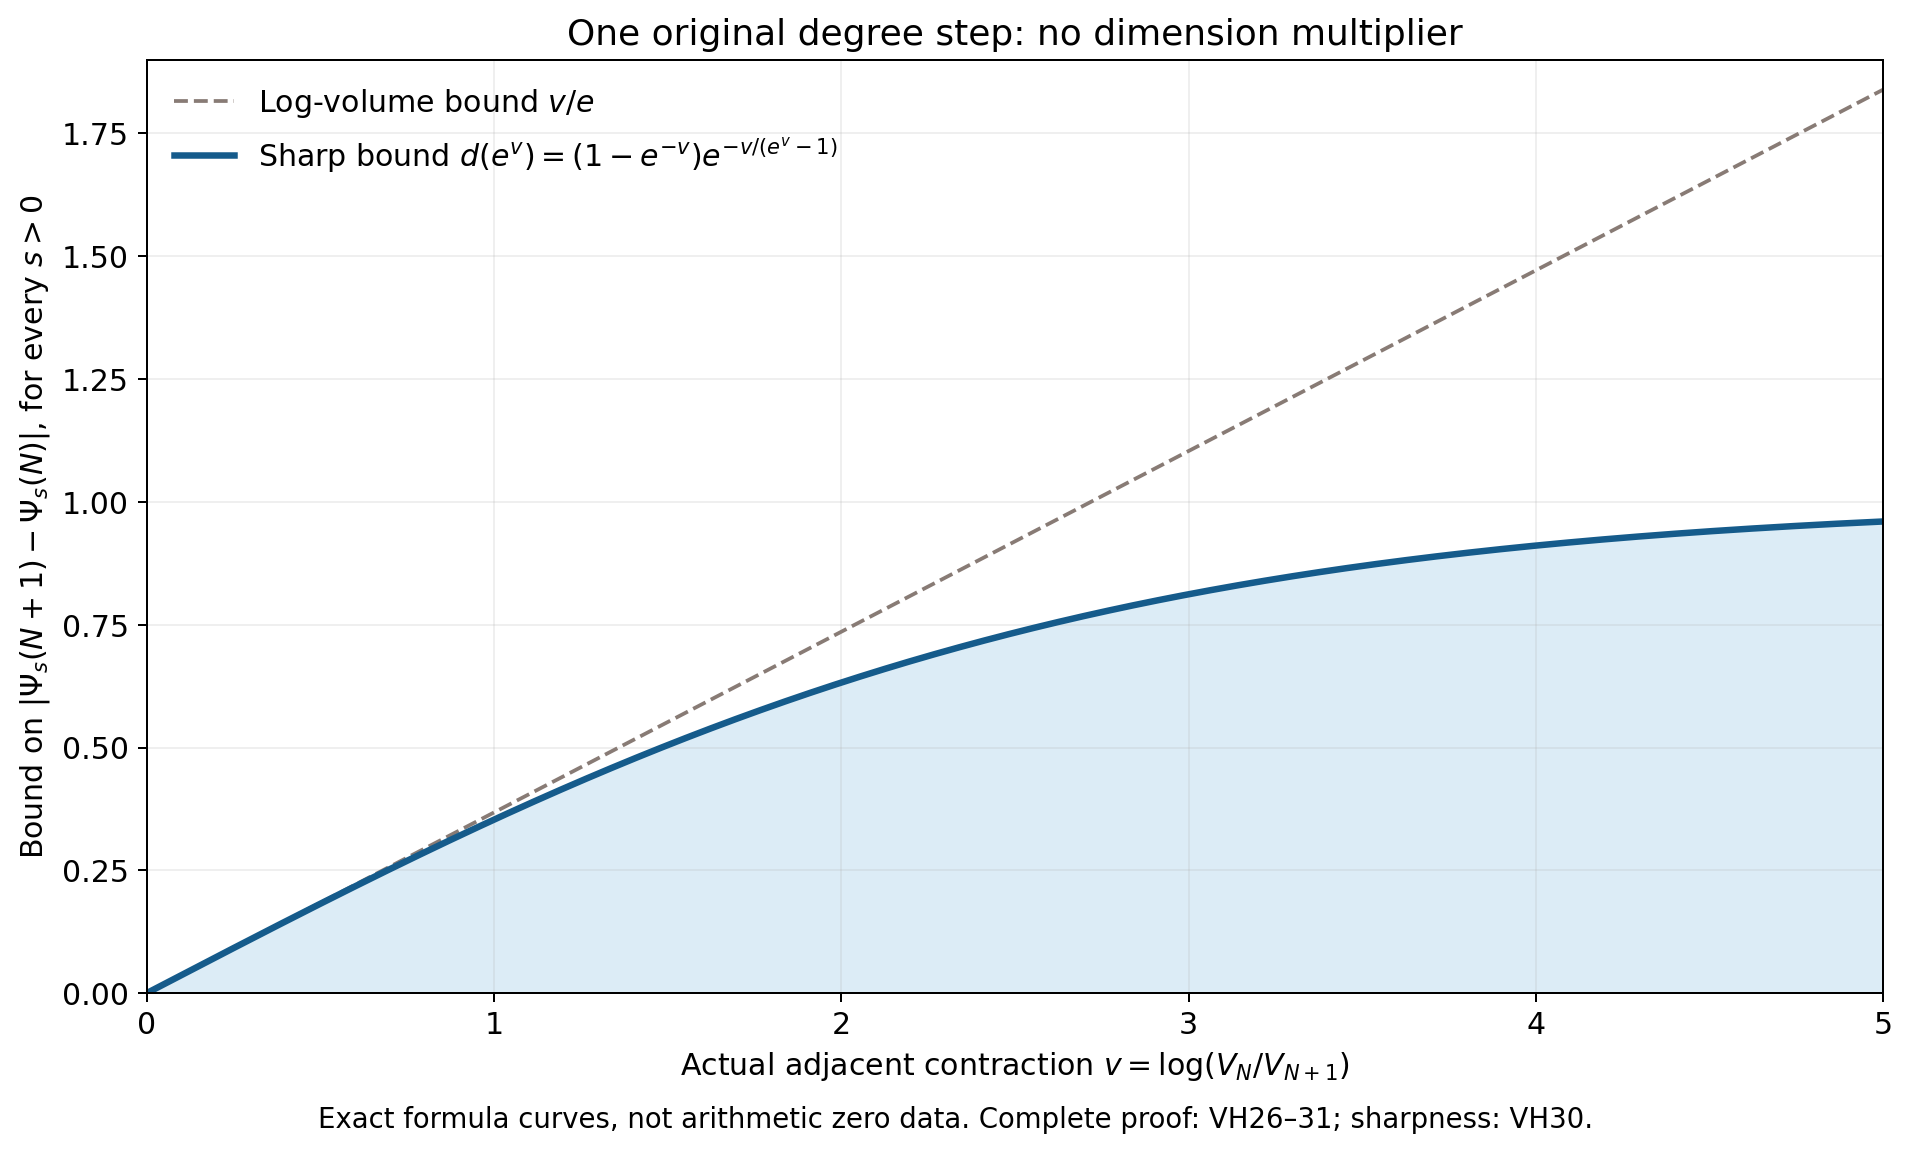
\includegraphics[width=\textwidth]{figures/degree_volume_heat.png}
Here $v=\log(V_N/V_{N+1})$ is the actual adjacent quotient-volume contraction.
For the original $M=(M_S-kI/2)/i$ and every $s>0$, the absolute change
of $\operatorname{tr}e^{-sM^{\dagger_{G_N}}M}$ is bounded by
$(1-e^{-v})\exp[-v/(e^v-1)]\le v/e$, continuously zero at $v=0$.
No dimension multiplier occurs. These are exact formula curves, not
arithmetic zero data or a confidence region. Complete proof: VH26--31;
general-matrix equality examples: VH30. The Gaussian heat context is
Alain Connes, \emph{Heat Expansion and Zeta}, arXiv:2402.13082v1,
equation ft. The finite receiving argument is proved in full above.
\clearpage
\section*{The exact theta transport and its observations}
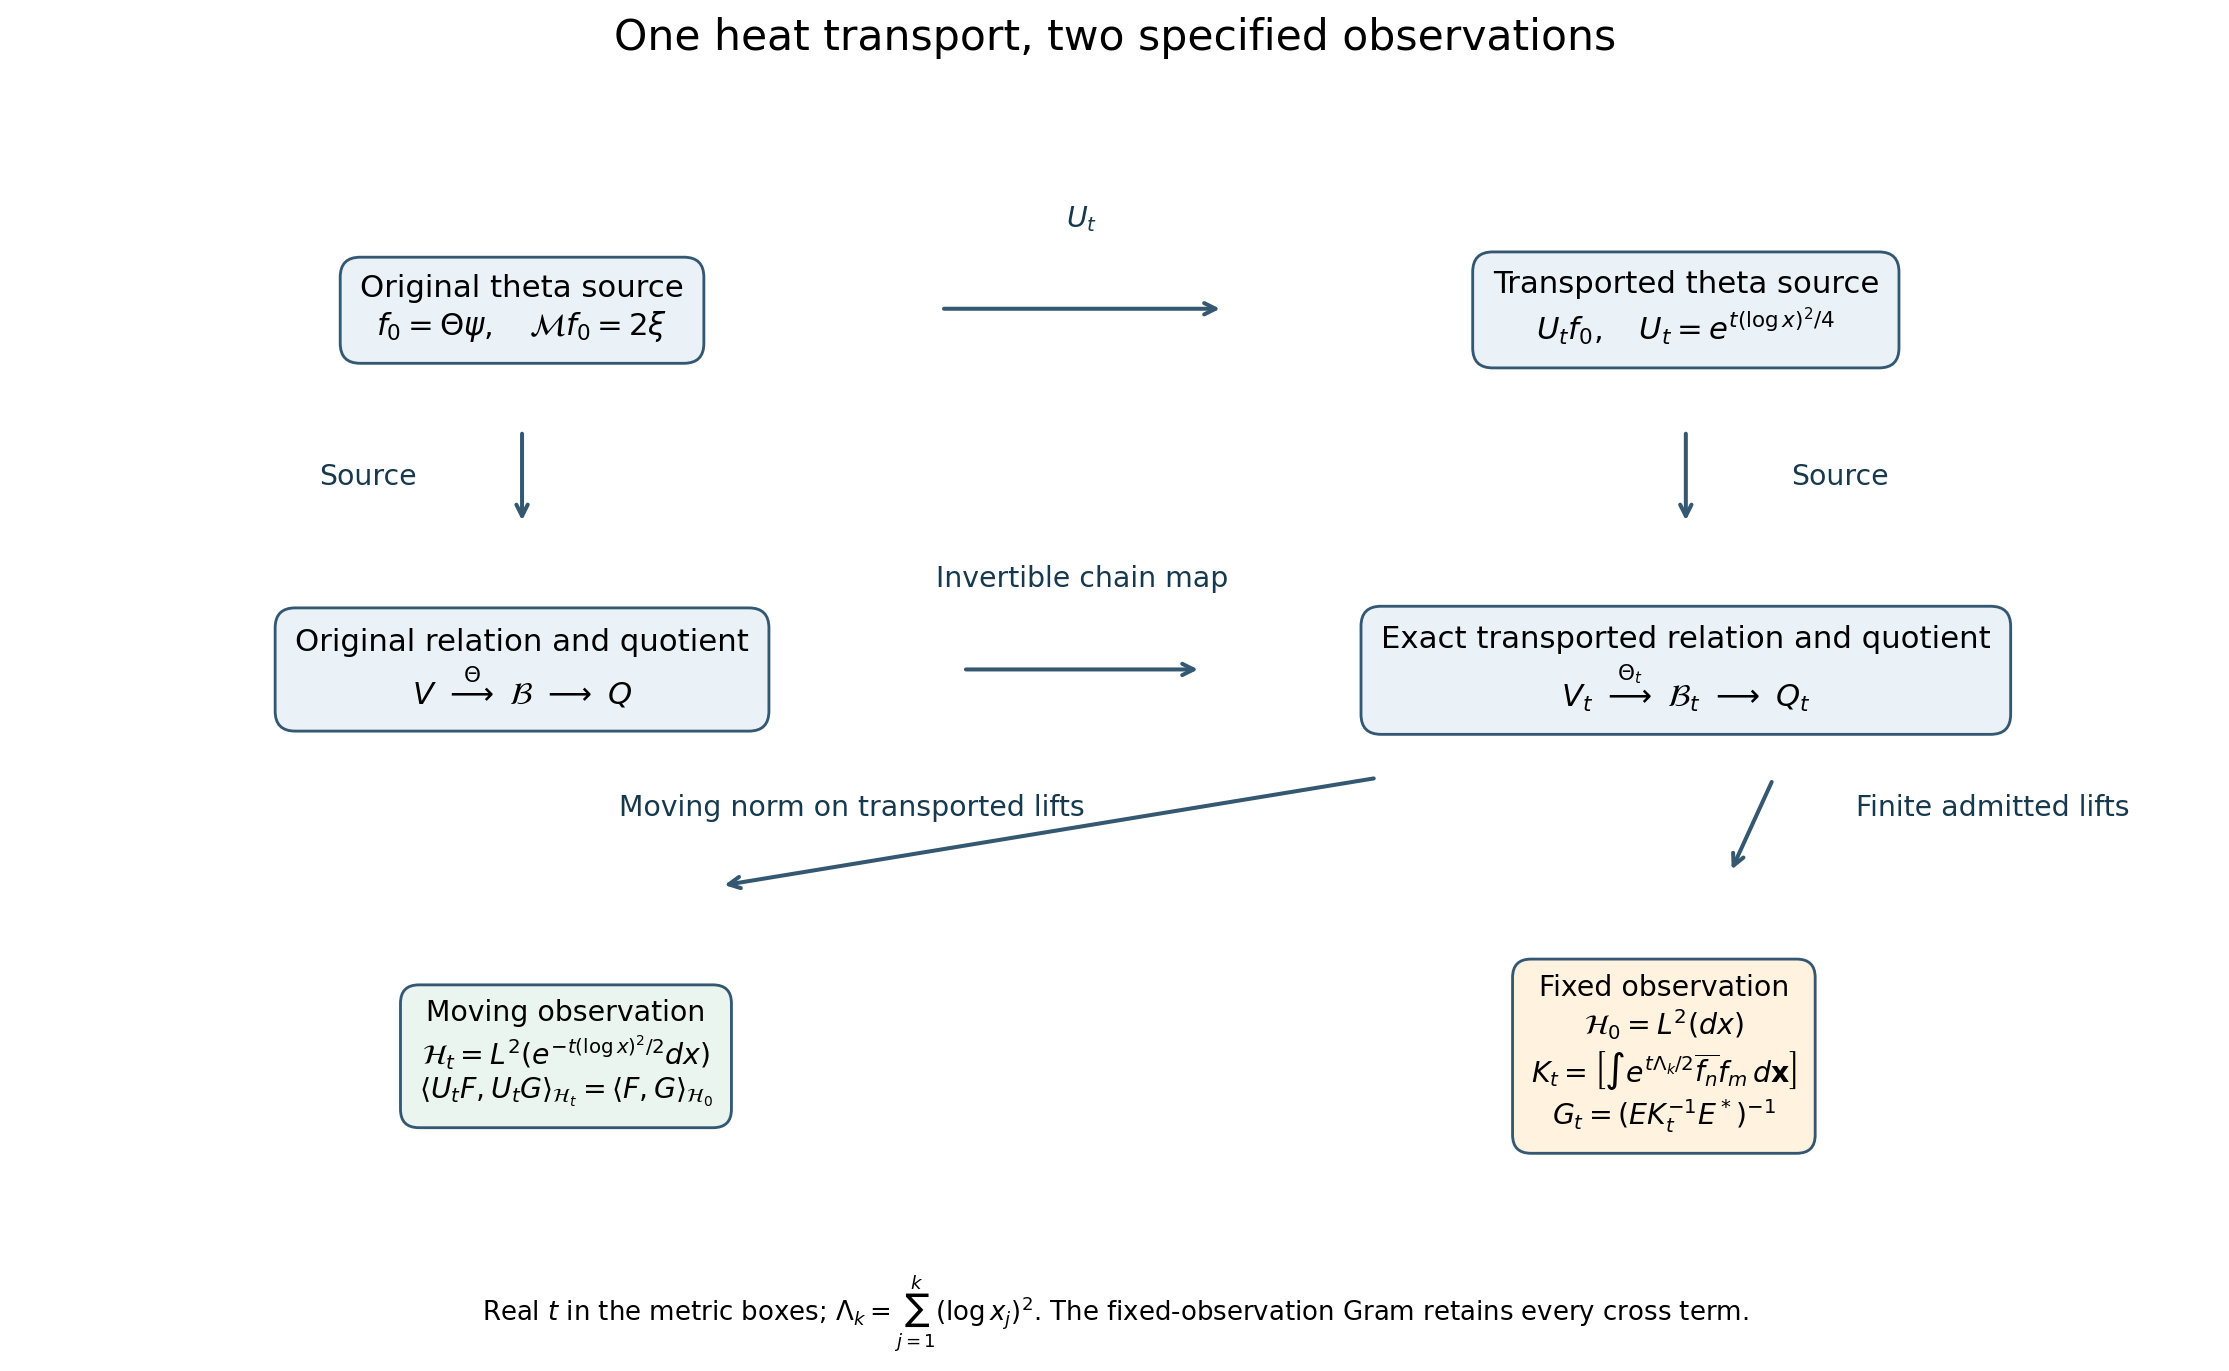
\includegraphics[width=\textwidth]{figures/theta_transport.png}
The diagram shows the source transport $U_t=e^{t(\log x)^2/4}$ and
the chain map $\Theta_t=U_t\Theta U_{-t}$ on their transported strong
spaces. Its observation branches concern the admitted source lifts,
not a map of the whole quotient into ambient $L^2$.
For real $t$, the moving measure is $e^{-t(\log x)^2/2}dx$.
The fixed measure remains $dx$; its finite tensor Gram uses
$\Lambda_k=\sum_j(\log x_j)^2$ and retains all complex products.
The complete transport and metric proofs above give every domain,
inverse and quotient map. Human source conventions: Alexander Dobner,
arXiv:2005.05142v2, equations eq:fourier, eq:phisum, eq:xiFtdef;
Brad Rodgers and Terence Tao, arXiv:1801.05914v5, equations hoz,
phidef, htdef. This exact programme transport is derived above.
\endgroup
% END COMPLETE HEAT TRANSPORT AND VOLUME PROOFS

\end{document}
